\documentclass[a4paper, 12pt]{report}
\usepackage[a4paper, top=2cm , bottom=2cm , right=2cm , left=2cm ]{geometry}

\usepackage{graphicx} % Required for inserting images
\usepackage[T1]{fontenc}
\usepackage[english]{babel}
\usepackage[utf8]{inputenc}
\usepackage{titlesec}
\usepackage{xcolor}
\usepackage{amsfonts}
\usepackage{wrapfig}
\usepackage{amssymb}
\usepackage{amsbsy}
\usepackage{float}
\usepackage{soul}
\usepackage[makeroom]{cancel}
\usepackage[framemethod=tikz]{mdframed}
\usepackage{mathtools}
\usepackage{matlab-prettifier}
\usepackage{subcaption}
\usepackage{bm}
\usepackage{tikz}
\usepackage{colortbl} % for cell color in matrices
\usepackage{booktabs}
\usepackage{amsmath}
\usepackage{xcolor}
\usepackage{tcolorbox}
\usepackage{tikz} %for block diagrams
\usepackage{amssymb}
\usepackage{enumitem} 
\usetikzlibrary{positioning}
\usepackage{xcolor}

\definecolor{myblue}{RGB}{30, 131, 197}
\definecolor{mygreen}{HTML}{25da18}
\definecolor{myyellow}{RGB}{255, 255, 0}
\definecolor{mygrey}{RGB}{100, 100, 100}
\definecolor{myred}{RGB}{255, 55, 55}

\newtcolorbox{factbox}[1][]{
    colback=mygreen!5,   % Background color
    colframe=mygreen!30, % Frame color
    fonttitle=\bfseries,  % Title font
    title=#1,             % Title
    coltitle = black,   %title color
    sharp corners=southwest,
}
\newtcolorbox{QandAbox}[1][]{
    colback=myred!5,   % Background color
    colframe=myred!20, % Frame color
    fonttitle=\bfseries,  % Title font
    title=#1,             % Title
    coltitle = black,   %title color
    sharp corners=southwest,
}

\newtcolorbox{example}[1][]{
    colback=mygrey!3,   % Background color
    colframe=mygrey!20, % Frame color
    fonttitle=\bfseries,  % Title font
    title=#1,             % Title
    coltitle = black,   %title color
    sharp corners=southwest,
}
% Do not indent paragraphs
\usepackage[parfill]{parskip}

\lstset{
    basicstyle=\ttfamily\scriptsize,
    keywordstyle=\color{blue},
    commentstyle=\color{green!60!black},
    stringstyle=\color{red},
    numbers=left,
    numberstyle=\tiny,
    stepnumber=1,
    numbersep=8pt,
    frame=single,
    breaklines=true,
    captionpos=b
}


% In case of an image at the bottom, but the footnote below the image (without this the image will be below the footnote)
\usepackage[bottom]{footmisc}

% --------- CUSTOM HEADER ----------
% Modifies the style of the header
\usepackage{fancyhdr}         
\pagestyle{fancy}
\fancyhf{}

% Sets as header: curr_section <space> page_number
\lhead{\rightmark}
\rhead{\textbf{\thepage}}

% Removes the page number at the beginning of chapters
\fancypagestyle{plain}{
  \fancyfoot{}
  \fancyhead{}
  \renewcommand{\headrulewidth}{0pt}
}

% Do not capitalize section name in header
\renewcommand{\sectionmark}[1]{\markright{\thesection.\ #1}{}}

% ------------ NEW ENVS ------------
% ---------- Proof environment ----------
\newenvironment{proof}
{\begin{mdframed}[leftmargin=15pt, rightmargin=15pt, leftline=false, rightline=false] \textit{\underline{Dim.}} \\[10pt] \textit\bgroup}
{\egroup \par \raggedleft $\square$ \end{mdframed}}

% Proof without top and bottom borders
\newenvironment{proof2}
{\vspace*{10pt} \begin{mdframed}[leftmargin=15pt, rightmargin=15pt, leftline=false, rightline=false, bottomline=false, topline=false] \textit{\underline{Dim.}} \\[10pt] \textit\bgroup}
{\egroup \par \raggedleft $\square$ \end{mdframed}}

% ---------- Addendum environment ----------
\newenvironment{addendum}
{\begin{mdframed}[leftmargin=15pt, rightmargin=15pt, leftline=false, rightline=false] \textit\bgroup}
{\egroup\hfill $\diamond$\end{mdframed}}


% ---------- NEW COMMANDS ----------
% ---------- Circled number ----------
\newcommand*\circled[1]{\tikz[baseline=(char.base)]{\node[shape=circle,draw,inner sep=2pt] (char) {#1};}} % 

% ---------- Real numbers and complex numbers shortcuts ----------
\newcommand{\R}{\mathbb{R}}
\newcommand{\C}{\mathbb{C}}




% Make references clickable and change style of links to blue
\usepackage{hyperref}
\hypersetup{
	colorlinks=true,
	linkcolor=blue,
	filecolor=magenta,      
	urlcolor=cyan,
}

\graphicspath{ {images/} }

\titlespacing{\title}{10pt}{50pt}{50pt}
\titlespacing{\chapter}{0pt}{10pt}{10pt}
\titlespacing{\section}{0pt}{35pt}{10pt}

\title{
    \textbf{\Huge{Laboratory of Robust Identification and Control}}\\
    \textit{Lecture notes}
}
\author{A. Ayanmanesh Motlaghmofrad}
\date{A.Y. 2024/2025}


% Force all math to use \displaystyle by default
\everymath{\displaystyle}

\linespread{1.2} % Adjusts line spacing to 1.5

\begin{document}
\maketitle
\tableofcontents


% ---------------------------------------------------------------------
% ------------------------ MODIFY ONLY BELOW --------------------------
% ---------------------------------------------------------------------
% ---------------------------------------------------------------------

\chapter{Introduction}    % For a new chapter (works in book and report class)
\subsubsection{Disturbances and uncertainties}
% page1
% -------------------------------------

    The key word \textit{Robust} suggests that we are taking uncertainties into account. The model of the plant is as following:

%Graph
\begin{figure}[htbp]
    \centering
    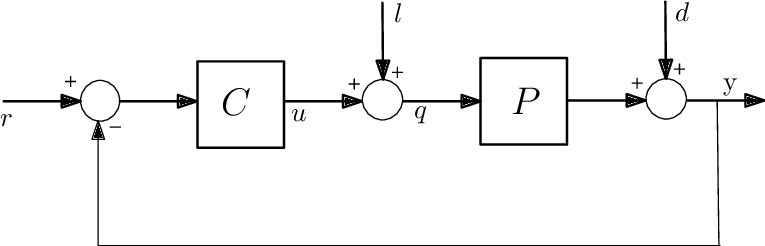
\includegraphics[width=\textwidth]{images/1.png} % Adjust width as needed
    \caption{A general control plant with additive disturbances \textit{l} and \textit{d}}
    \label{fig:graph_label}
\end{figure}


The general nonlinear state-space representation of the system is:

\begin{equation}
    \begin{cases}
    \dot{x}(t) = f(x(t), u(t)) \\
    y(t) = g(x(t), u(t))
    \end{cases}
\end{equation}
Where:
\begin{itemize}
    \item $x(t)$ is the state vector,
    \item $u(t)$ is the input vector,
    \item $y(t)$ is the output vector,
    \item $f(\cdot)$ is a nonlinear function describing the system dynamics,
    \item $g(\cdot)$ is a nonlinear function describing the output equation.\\
\end{itemize}

%page 2
%--------------------------------------------------
    \textbf{The first step} of any control problem is typically \textbf{derivation of mathematical model of the plant.} This step is the most crucial step, because if we drive the model by applying first principles of physics, we are likely to adopt approximated models, adopting simplifying assumptions, e.g. rigid body assumption etc. Further, the value of the physical parameters involved in the equations, such as friction coefficient, are not exactly known. Such approximations introduce errors and uncertainty in the mathematical description of the plant to be studied and controlled.

% page 3
% -----------------------------------------------------
    This fact is critical, since standard approaches to controller design are model-based; that is, the controller design has a strong dependency on the mathematical models used to describe the plant to be studied and controlled.


\begin{center}
$\textit{\textbf{Neglecting some physical details}} \equiv \textit{\textbf{Neglecting some state variables}}$
\end{center}

    For example, for modelling a robotic arm, generally, rigidity is assumed for the joints. Nevertheless, in fast movements  this assumption does not hold anymore, and the model does not predict the real performance of the robot, neglecting some state variables. Further, in some applications, we are not even aware of the phenomenon or phenomena that is being neglected. 

\subsubsection{Counter act for disturbances and uncertainties}

\begin{itemize}
    \item \textbf{First counter act}  These uncertainties and disturbances directly affect the controller design in the time domain, since the feedback gain and observer are directly calculated by solving algebraic equations including physical parameters with uncertainties. Nontheless, In frequency domain, the design of the controller is less affected by these uncertainties. 

    This does not mean that \textit{Transfer Function} is not affected by uncertainties of the parameters, because not considering some phenomona leads to the transfer function having less poles or zeros and because the uncertainty of the parameters affect the coefficients of the complex variables, being \textit{s} or \textit{z}. In the frequency domain design, we design the controller based on the frequency response of the system, considering cutting frequencies that reject high-frequency and low-frequency disturbances. In addition, by considering phase-margin and gain-margin, some margin for disturbances and uncertainties are taken into accoutn.

\textbf{Question to be answered: the sensitivity function is high-pass filter, meaning that the high frequency phenomenon, on the other-hand T is a low-pass filter, if the plant is designed for having a fast rising time, high-frequency phenomena also passes T.}

    \item \textbf{Second counter act}: Optimization problems in state-space where introduced to tackle this problem.
    \item \textbf{Third counter act}: Optimization problem, in state space, is combined with the concept of robustness, in frequency space, which is called $H_{\infty}$. 
\end{itemize}


\subsubsection{What is going to be discussed in this course}
    In the first part of this course, we are going to learn how to learn from the mapping from the input to the output of the system, extracting a \textbf{mathematical model} for the plant. Further, it elaborates on this data to drive also a \textbf{discription for uncertainty}. These, together, can be used for \textbf{robust controller design} in a model-based approach.

    In the second step, the aim is to design a controller directly from the data, without the intervention of the model.


\begin{factbox}[Professor's Quote]

    In conclusion, even if the physical model is very precise, at some point, in order to measure the parameters used in the physical models, it is required to do some experimental measurements, subjected to noise, introducing uncertainties to our model.\newline \newline
    If these uncertainties are not taken into account, the controller will not have a good performance when implemented physically, and it is going to work only in simulations. \newline \newline
    There are many approaches to tackle this problem. Here, in the first part of the course, we will focus on \textbf{System Identification}, which is another modelling paradigm. In this paradigm, we learn the mathematical model of the system to be controlled by using experimentally collected data. Not only do we introduce what \textit{System identification} is and what are the possible approached, but maintly to focus on \textbf{\textit{Set-membership Identification Technique}} that allow us to learn the model of the system, and drive information about how the uncertainty is affecting out model; this is used to design a controller in a robust manner. Robust controller designed can be directly applied to the real physical plants.  \newline \newline
    
    In the second part of the course, we shift our paradigm again. In this part, assuming that the collected data represents the behavior of the mapping between the input and output, we try to design the controller directly from the data, called  \textbf{Direct Data-Driver Controller Design}. \newline \newline
    
\end{factbox}

\textit{System identification} deals with the problem of building mathematical model of dynamical systems from sets of experimentally collected input, output data.


\begin{figure}[htbp]
    \centering
    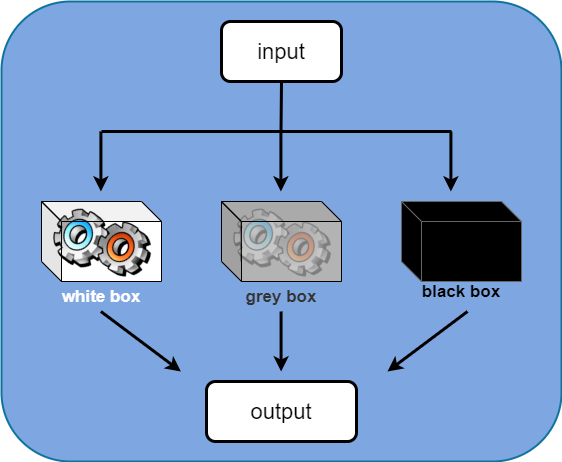
\includegraphics[width=0.5\textwidth]{images/system-id-scheme.png}
    % Adjust width as needed
    \caption{Classifications of System Identification Problems}
    \label{fig:id_classes}
\end{figure}

There are three different approaches to mathematically model dynamical systems:
\begin{enumerate}

\item \textbf{White-box modelling}:\newline Models, in this approach, are obtained by applying \textbf{first principles for physics}. All the physical phenomena and also all the physical parameters involved in the equiation are assumed to be exactly know. This approach was applied in the course of \textit{Automatic Control} for modelling systems.

\item \textbf{Grey-box modelling}: Here, \textbf{models} are base on the equations obtained by applying first principles of \textbf{physics}, but \textbf{the parameters} entering the equations are not completely known, so they need \textbf{to be estimated} from experimental data. 

\item \textbf{Black-box modelling}: In this case, the structure of the equations is selected by the user on the basis of some \textbf{"general" a-priori information}, e.g. linearity, on the system physics, or at any rate by the system properties. \newline 

\begin{factbox}[Professor's Quote]
    In this method, the designer of the system model, has some degree of freedom in selecteing the structure of the model, provided that the model embeds the "general" a-priori information.\newline \newline
    If we do not have any a-priori information, an artificial-neural-network may be selected as the structure of the model.
\end{factbox}
the parameters involved in the equations of the black-box models are \textbf{to be estimated}, or computed, by using experimentally collected data. In general, \textbf{the parameters of a black-box model do not have a clear physical meaning}.
\end{enumerate}


In general, \textbf{white-box models are not very useful in practice}, at least for control applications, because they are based on the assumption that the physics involved in the system under study is well-known.

\subsubsection{The comparison between the grey-box and Black-box models:}
\textbf{Similarity} 
In both cases:
\begin{itemize}
\item physical insight is exploited to drive/select the structure of the equations.
\item experimentally collected data is used to estimate/compute the parameters involved in the equations.
\end{itemize}

\textbf{Difference} 
\begin{itemize}
\item In grey-box modelling, the structure of the equations is not selected by the user, since it is forced by the first principles of physics. This suggests that, in general, the equations of a grey-box model depends, in a possibly complex, non-linear ways, on the physical parameters to-be-estimated.\newline
for instance of a grey-box model:
$\begin{cases}
    \dot{x}(t) = A x(t) + B u(t) \\
    y(t) = C x(t) + D u(t)
\end{cases}$ where:
\newline
\[
A = \begin{bmatrix}
\frac{m}{k^2} & \sqrt{\beta}\\
\frac{\alpha^2.k^3}{\gamma} & 1  
\end{bmatrix}, \quad
B = \begin{bmatrix}
b_1 \\
b_2
\end{bmatrix}, \quad
C = \begin{bmatrix}
c_1 & c_2
\end{bmatrix}, \quad
D = \begin{bmatrix}
d
\end{bmatrix}
\]
In this case, using the physical principles for modelling seems like a good idea; the system is simple, and its physics is well-known. The problem is that the parameters are to-be-estimated. This problem leads to an optimization problem. Now, A difficulty may arise, because if the equation we are going to write so that they relates input and output data obtained experimentally depends on parameters in a complex and non-linear fashion, the mathematical problem of driving what are the correct value of the system parameter satisfying the relation between the intput and output is going to be a complex problem. \textbf{This is the main limitation of grey-box model.}

\item In the black-box version of the same problem, just some general information such as liniearity and time-invariantion is exploited. Now, we found the four matricies \textit{A, B, C, D} in a form that is much simpller, just 4 parameters for A, and so on, for instance. In this case, the system output depends on the input in a way simpler manner.
\[
A = \begin{bmatrix}
a_{11} & a_{12} \\
a_{21} & a_{22}  
\end{bmatrix}, \quad
B = \begin{bmatrix} 
b_1 \\
b_2
\end{bmatrix}, \quad
C = \begin{bmatrix}
c_1 & c_2
\end{bmatrix}, \quad
D = \begin{bmatrix}
d
\end{bmatrix}
\]\newline


\begin{factbox}[Professor's Quote]
    Therefore, in black-box model, we have more freedom to select the struture of the equations in a way that is computationally more convenient, by embedding/exploiting some general properties drived from our physical insight. 
The idea is to consider only the most important a-priori information and/or the information that we trust the most!
\end{factbox}

\end{itemize}

\subsubsection{General procedure for building a grey/black-box modelling:}
Let's compare grey-box and black-box models from the point of view of the parameter estimation problem. While building the mathematical model of the system, in general, we follow a procedure similar to the following one, it be a grey-box or black-box structure:\newline

\begin{enumerate}
    \item to exploint availabe a-priori information on the system under study to select \textbf{the structure of the mathematical equation} describing the input-output mapping.
    \begin{factbox}[Professor's Quote]
The model is always in the input/output form. Signals that we can apply to the system is called input, and signals that we can measure, is called output. If we are in the case where we can measure all \textbf{state variables} involved in the system, we can have a full description of the system. However, in a general case, the system involves input, output, and state variables, but we are able to measure only a subset of physical variables in the system - being the value to be monitored or the control output.

Now, these parameters have physical meaning in grey-box case, or are merely mathematical parameters in black-bock case.
\end{factbox}

In the end of this step, we have a mathematical model of the following form:
\begin{equation}
y(t) = f\left( u(t), \theta\right)
\end{equation}

    \item To collect input-output data representing the behavior of the system under study by performing an experiment. $\tilde{u}$ and $\tilde{y}$ are noise-corrupted data, since, in general, noise can corrupt the output measurements as well as measurement of the input signal applied to the system.
\begin{center}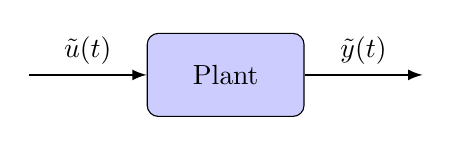
\begin{tikzpicture}[auto, node distance=2.5cm, >=latex]
    % Define styles
    \tikzstyle{block} = [rectangle, draw, fill=blue!20, 
                          text width=5em, text centered, rounded corners, minimum height=3em]
    \tikzstyle{input} = [coordinate]
    \tikzstyle{output} = [coordinate]
    \tikzstyle{arrow} = [thick,->,>=latex]
    
    % Nodes
    \node [input] (input) {};
    \node [block, right of=input] (plant) {Plant};
    \node [output, right of=plant] (output) {};
    
    % Draw arrows
    \draw [arrow] (input) -- node [above] {$\tilde{u}(t)$} (plant);
    \draw [arrow] (plant) -- node [above] {$\tilde{y}(t)$} (output);
\end{tikzpicture}\end{center}
    \item To formulate a suitable mathematical problem to estimate/compute the values of the vector of parameters $\theta$ in such a way that our mathematical model is going to describe the behavior of real system as well as possible.
for example:
\[
\hat{\theta} = \arg \min\limits_{\theta \in S} f(\theta) = \arg \min\limits_{\theta} \|\tilde{y} - f(\tilde{u}, \theta)\|_2
\] 
J(.) here is a \textbf{cost function}. In this case, it is the euclidian norm of $\tilde{y}$ and $f(\tilde{u}, \theta)$.\\
\end{enumerate}
\newpage
At the third stage, the difference between grey-box and black-box models comes into play, since:
\begin{itemize}
    \item In grey-box model: $f(\tilde{u},\theta)$ will, in general depends in a complex, non-linear manner from $\theta$, \textbf{leading to multi-minima convex cost function which is really hard to be minimize}\\ \\
    While\\
    \item In black-box model: $f(\tilde{u},\theta)$ will be selected by the user in order to depend linearly from $\theta$,if possible, or in the simplest possible way, \textbf{leading to a single-minima convex funciton to be minimized}, which is much easier in comparison. \\
\end{itemize}
For example, consider the following multi-minima cost-function: \\

\(
J(\theta_1, \theta_2) = \sin(\theta_1) \cdot \cos(\theta_2) + \frac{\theta_1^2 + \theta_2^2}{10}
\)

\begin{figure}[htbp]
    \centering
    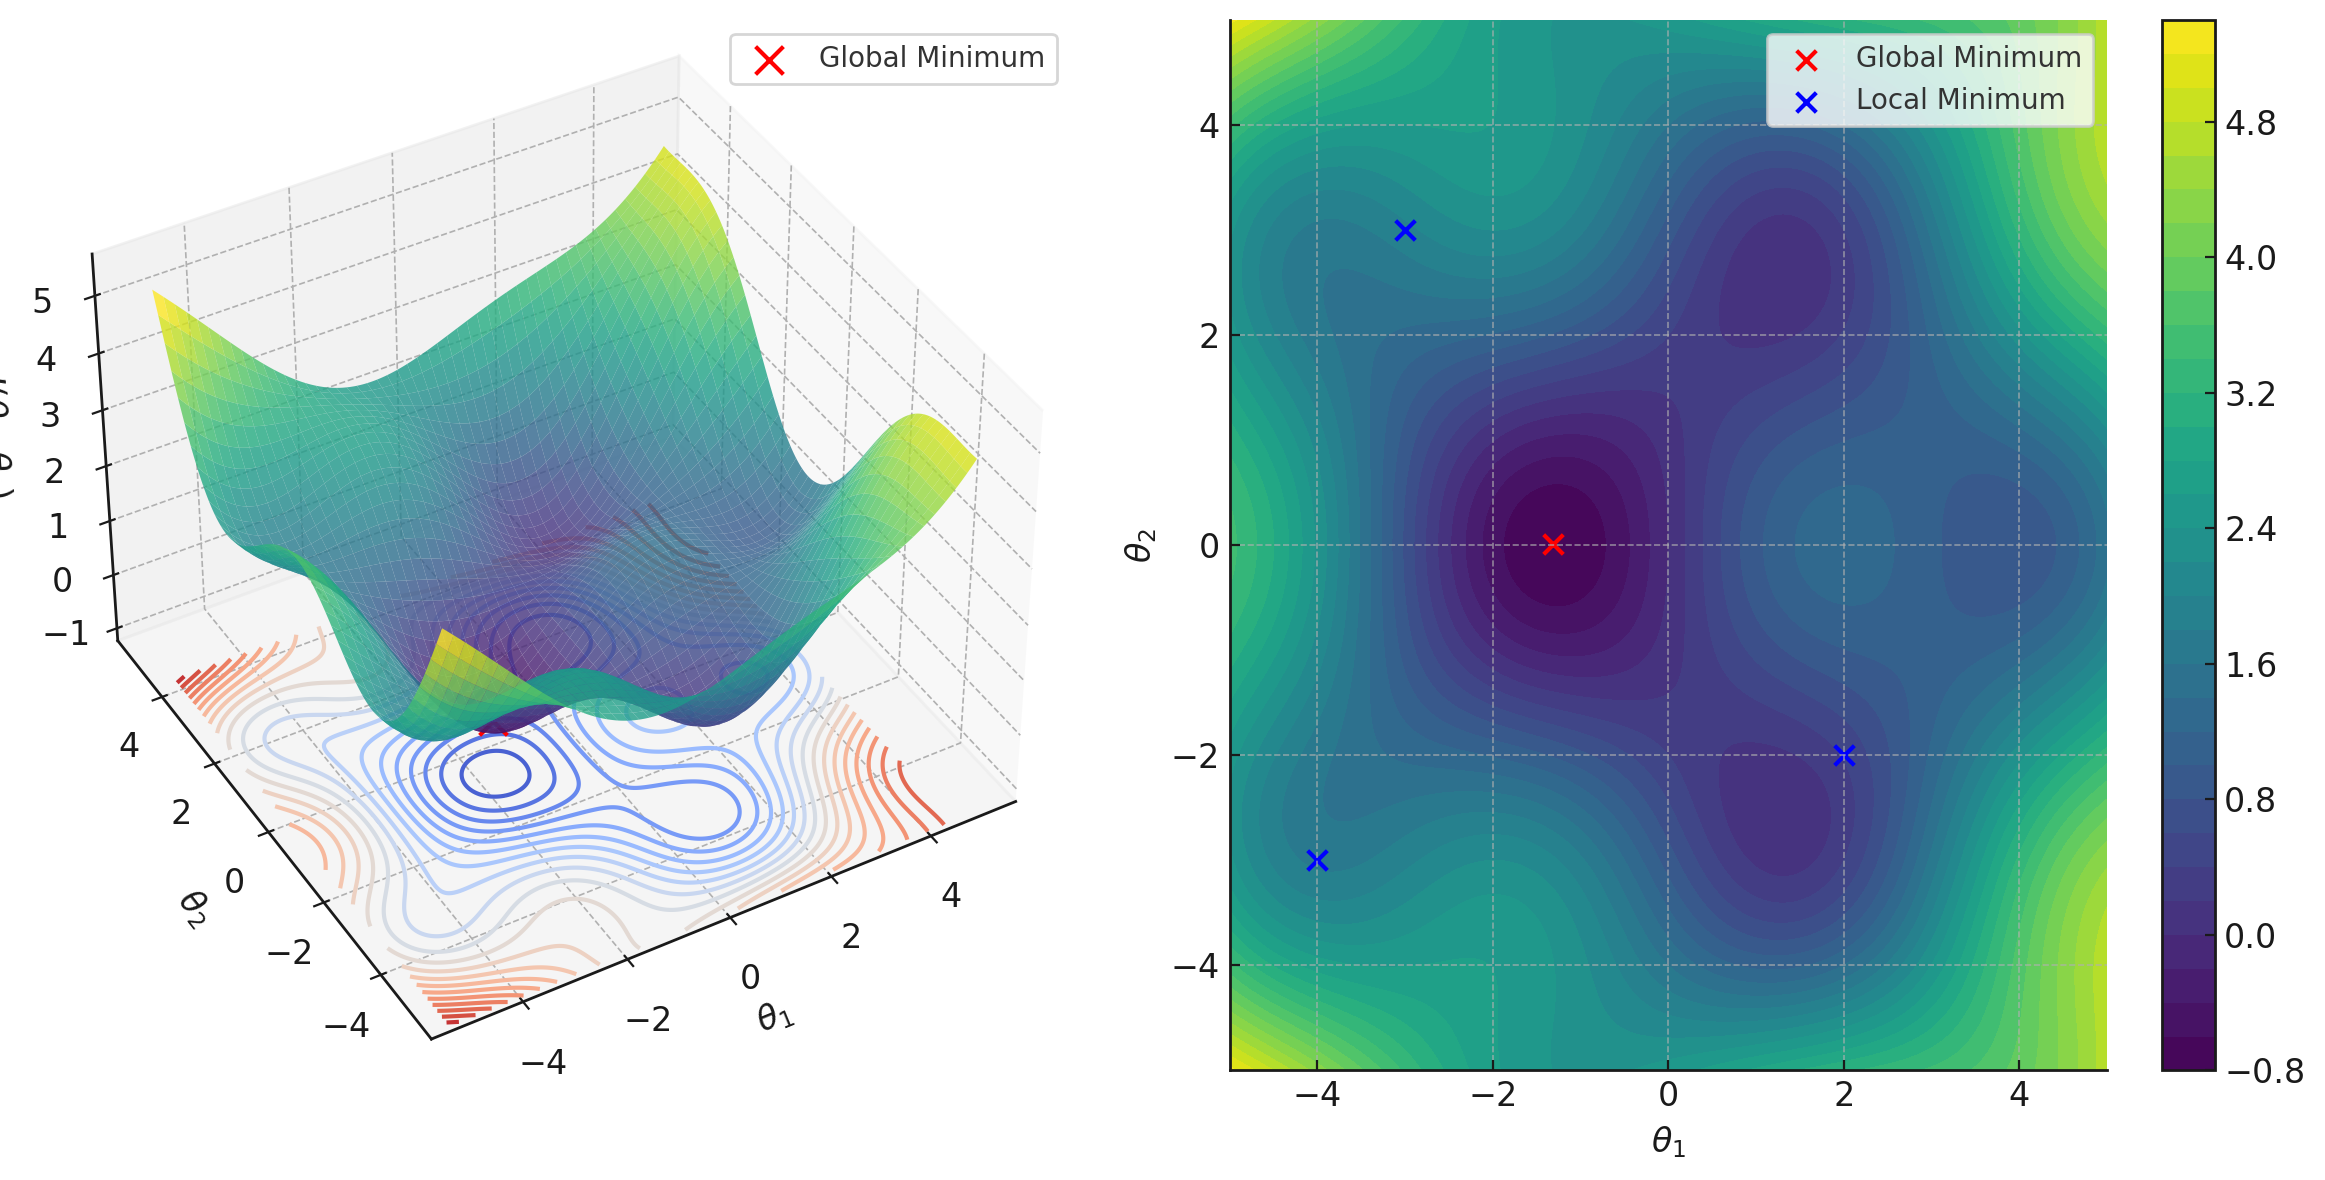
\includegraphics[width=0.75\textwidth]{images/multi-minima-cost-function.png}
    % Adjust width as needed
    \caption{The 3D plot and countor plot of the afforementioned cost-function, which is a multi-minima cost-function}
    \label{fig:multi-minima-cost-function}
\end{figure}

In this example, we look for the global minimum of the cost-function. Finding this point, however, is not an easy task, due to the fact that there is no guarantee that our optimization algorithm will not be trapped in one of the local minima, which may correspond to a "very bad" estimation of $\theta$. Even if we find the global minimum by chance, there is no guarantee that output is indeed the global minima.

On the other hand, When a black-box model is considered, a parametrization is considered so that the function $f(u,\theta)$ is a convex function of $\theta$, thereby having a single global minimum. In this case, no matter what optimization algorithm is used, reaching the global minimum is guaranteed.This is evident in the following cost-function:\\

\(
J(\theta_1, \theta_2) = \theta_1^2 + \theta_2^2
\)
    
\begin{figure}[htbp]
    \centering
    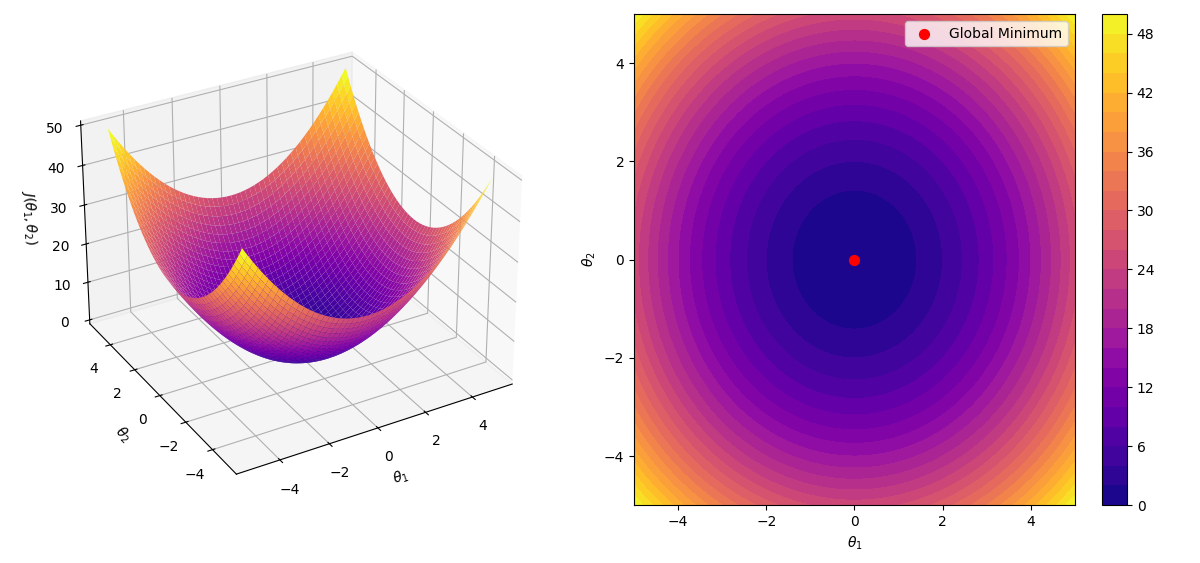
\includegraphics[width=0.75\textwidth]{images/convex-cost-function.png}
    % Adjust width as needed
    \caption{The 3D plot and countor plot of the afforementioned cost-function, which is a convex cost-function}
    \label{fig:multi-minima-cost-function}
\end{figure}


\begin{QandAbox}[Q and A]
    \textbf{Question:} we use grey-box model when we have an insight about the system and parameters. Hence, when we run the optimization problem, we can initialize the optimization problem with more suitable initial condition. Further, we can neglect some of the estimation, knowing that the estimated value does not correspond to the physical quantity the parameter is expected to have.\\
    
    \textbf{Professor's answer:} This is true for simple systems. Nonetheless, in such compolex systems as chemical processes or optical lazer systems, it's hard to have an insight before hand about some parameters. In addition, since we are dealling with multi-dimensional problems, it might be the case that we confine the expected value for some parameters but still, for some parameters, we need to deal with the issue mentioned about the multi-minima cost functions. However, it might be the case that the estimation of those physical parameters are of interest, which is not the concern of this course. Here, we do system identification for control purposees. \\
    
\end{QandAbox}

To clarify the matter further, consider an \textbf{\textit{LTI system}} such that the \textbf{transfer function} obtained from \(H(s) = C (sI - A)^{-1}B +D\) where matrices \(A, B, C, D\) are teh state-space matrices obtained by applying the first principles of physics.\\

\(
H(s) = \frac{ \frac{P_1²}{P_2} s + \frac{P_3}{\sqrt{P_4}}}{s^2 + \frac{P_1.P_2}{P_3^3} + 1}
\)\\

Where \(P_1, P_2, P_3, P_4\) are the physical parameters. Now, in terms of modelling the input-output behavior of the system, we don't miss anything by considering the following transfer function.\\

\(
H(s) = \frac{\theta_1 s + \theta_2}{s^2 + \theta_3 s + \theta_4}
\)\\

In this black-box model, we just take into consideration the most important "general" information that the system is an LTI system - hence being able to be modelled as a transfer function - and of order two. Therefore, we can use a transfer function model for describing the system behavior. State-space models can be obtained from transfer functions by applying basic results on \textbf{\textit{realization theory}}, which is not going to be discussed in this course.\\

\begin{factbox}["Phylosophical Remark"]
    Pay attention that \textbf{we cannot build our model without any assumption about the system}. No matter how much input-output sample is available,  we need to have an assuption about the system to be able to descibe it.
\end{factbox}

In conclusion: \\
\textbf{black-box models} are thet best choice for the following purposes:
\begin{itemize}
    \item simulalting the input-output behavior of the system
    \item modelling for the purpose of designing a controller\\
\end{itemize}

\textbf{Grey-box models}, in general, are the best choice when it is desired to:
\begin{itemize}
    \item estimate the values of some physical parameters \\
\end{itemize}

If the physical systeme is well-known, \textbf{white-box modelling} is the choice.

\chapter{System Identification}    % For a new chapter (works in book and report class)
\subsubsection{Generalities}


Since experimental measurement procedure typically provides samples of input-output sequences, we start by considering identification of \textbf{\textit{discrete-time models}}. Procedure for identifying \textit{\textbf{continous-time models}} will be dicussed as well.\\
Here, we are dealling with \textbf{dynamical systems}. A system is called dynamic when its output at a given time is dependent on the all the inputs that have been inserted to the system up to that time, or equivalently we know the value of the input at the previous time-instance in and the initial value of the a set of variables called, \textbf{\textit{state variables}}.

The choice of state variables is not unique, but the number of them depend on the order of the system. It can be proved that \textbf{a possible choice for state variables is previous values of the output}.

It is assumed that, without loss of generality, any system, be linear or non-linear, can be modelled by means of the following \textit{\textbf{regression form}}:\\
\begin{equation}
y(k) = f(y(k-1), y(k-2), \cdots, y(k-n), u(k), u(k-1), \cdots, u(k-m), \theta_1, \theta_2, \cdots, \theta_{n+m+1})
\end{equation}
\begin{itemize}
\item \(n\) is the system order, \textbf{related to the number of state variables}
\item \(m < n\), always for the physical, or at any rate, causal systems.
\item \(u(k), y(k), k = 1, 2, ..., H\) are the \textbf{noise-free} samples of the input and output sequences, respectively.\\
\end{itemize}

\begin{center}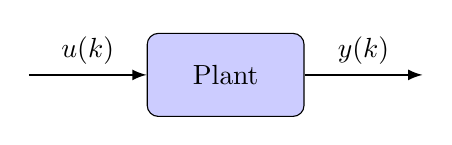
\begin{tikzpicture}[auto, node distance=2.5cm, >=latex]
    % Define styles
    \tikzstyle{block} = [rectangle, draw, fill=blue!20, 
                          text width=5em, text centered, rounded corners, minimum height=3em]
    \tikzstyle{input} = [coordinate]
    \tikzstyle{output} = [coordinate]
    \tikzstyle{arrow} = [thick,->,>=latex]
    
    % Nodes
    \node [input] (input) {};
    \node [block, right of=input] (plant) {Plant};
    \node [output, right of=plant] (output) {};
    
    % Draw arrows
    \draw [arrow] (input) -- node [above] {$u(k)$} (plant);
    \draw [arrow] (plant) -- node [above] {$y(k)$} (output);
\end{tikzpicture}\end{center}
\newpage

\subsubsection{General black-box EIV set-up}

\textit{Error-In-variables}, or EIV, problems refer to the most general case where both input and output collected samples are affected by noise, as represented in the figure \ref{fig:EIV}.\\
Two a-priori assumption is required at this point:\\
\begin{itemize}
\item a-priori assumption on the model: \(f \in F\) where \(F\) is a given class of functions
\item a-priori assumption on the noise: e.g. statistically distributed, or boundedness, etc
\end{itemize}
Then, we need to collect input-output data.
\begin{factbox}
\textbf{Without any assumption} about the noise corrupting the measurements, we cannot study the data at hand. Further, without any assumption about the structure, many structure can be find that map input samples to the output, that does not correspond to the behavior of the system. 
\end{factbox}

\begin{figure}[htbp]
    \centering
    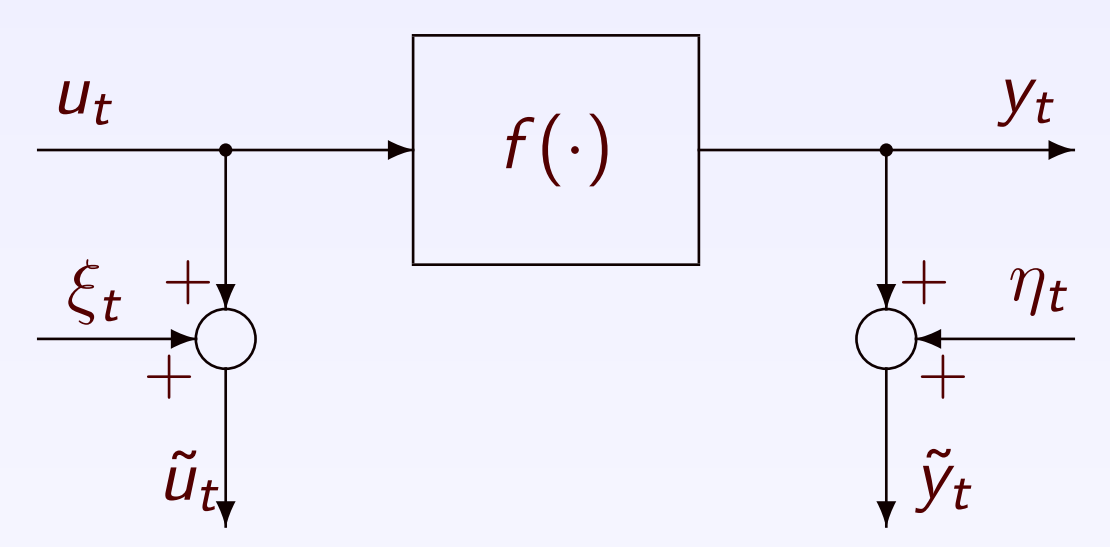
\includegraphics[width=0.5\textwidth]{images/EIV-problem.png}
    % Adjust width as needed
    \caption{a general shceme of error-in-variable problem}
    \label{fig:EIV}
\end{figure}

\subsubsection{A naive noiseless example}

Consider the following second order LTI discrete-time system (agent):

\begin{equation}
\begin{array}{l}
y(k) = f(y(k - 1), y(k - 2), u(k), u(k - 1), u(k - 2)) \\[1ex]
= -\theta_1 y(k - 1) - \theta_2 y(k - 2) + \theta_3 u(k) + \theta_4 u(k - 1) + \theta_5 u(k - 2)
\end{array}
\end{equation}

By introducing the backward shift operator \(q^{−r}\): \(q^{−r}(s(t))\)  = \(s(k − r)\), we can
rewrite the equation as:
\begin{equation}
y(k) = -\theta_1 q^{-1} y(k) - \theta_2 q^{-2} y(k) + \theta_3 u(k) + \theta_4 q^{-1} u(k) + \theta_5 q^{-2} u(k)
\end{equation}
Solving the equation in the \(y(k)\) we obtain:\\
\begin{equation}
y(k) = \frac{\theta_3 + \theta_4 q^{-1} + \theta_5 q^{-2}}{1 + \theta_1 q^{-1} + \theta_2 q^{-2}} u(k)
\end{equation}
By applying properties of the Z-transform it is possible to show that the system
transfer function G(z) can be obtained by simply replacing \(q^{-1}\) with \(z^{-1}\):
\begin{equation}
G(z) = \frac{Y(z)}{U(z)} = \frac{\theta_3 z^2 + \theta_4 z + \theta_5}{z^2 + \theta_1 z + \theta_2} u(k)
\end{equation}

Given H experimentally collected input-output samples matrix \ref{eq:regressor}, which is also called \textbf{\textit{regressor-matrix}}, leads to the following system of linear equations:
\begin{equation}
    y = A\theta
\end{equation}
where \(y = [y(3) y(4) ... y(H)]^T, \theta = [\theta_1 \theta_2 ... \theta_5]^T)\), and

\begin{equation}
    A = \left[
    \begin{matrix}
    -y(2) & -y(3) & u(3) & u(2) & u(1) \\
    -y(3) & -y(2) & u(4) & u(3) & u(2) \\
    \cdots & \cdots & \cdots & \cdots & \cdots   \\
    \cdots & \cdots & \cdots & \cdots & \cdots   \\
    -y(H-1) & -y(H-2) & u(H) & u(H-1) & u(H-2)
    \end{matrix} 
    \label{eq:regressor}
    \right]\\
\end{equation}

In this ideal, noise-free example, \(H = \text{the number of parameters} + \text{the order of the systerm}\), in this case, \(H = 7\) is enough to solve our 5-equations-and-5-unknown problem. The solution is going to be in the following form
:\\
\begin{equation}
    \theta = A^{-1} y
    \quad \overset{\text{Existence and Uniqueness Condition}}{\Rightarrow} \quad
    \begin{cases}
        
        A \in \mathbb{R}^{n \times n} \\
        \left|A\right| \neq 0
        
    \end{cases}
\end{equation}
One possible solution: apply to the system a random input sequence \(u\).\\

This formulation works for all the description that the output of the system is \textbf{linear with respect to the parameters}.

\begin{factbox}[Professor's Quote]
    In artificial-neural-network, the structure of \(f\) is different. Otherwise, the goal of any Machine Learning or System Identification problem is to find the mapping between the inputs and outputs.\\
    Regarding the importance of a-priori info about the system. The previous problem can also be solved for the following structure, that does no correspond to the behavior of a 2-order LTI system.
    \(y(k) = \theta_1 u(k) + \theta_2 u(k)^2 + \cdots + \theta_5 u(k)^5\)
\end{factbox}

\begin{example}[Example]
    It is desired to estimate the value of a resistor. A-priori info is that a resistor follows Ohm's law. As input signal, we insert current to our resistor and we measure the voltage across our resistor. \\
    
    \(y(k) = \theta u(k) \text{ s.th. y(.),u(.), }\theta \in \mathbb{R}\)\\
  
Here, \(\theta\) stands for the value of the resistor to be estimated. For this static system, which means the output of the system depends only on the values of the input at that time instance, we need a pair of noise-free input-output sample to estimate the value of the resistor. \\

\(\theta = \frac{y(1)}{u(1)}\)\\
\end{example}

\subsubsection{Noise effect}
If the measurements are corrupted by noise, the idea is to perform more measurements to average out the effect of the noise; \(H >> 2n + 1\) where n is the system order.\\

In this case, matrix\(A\) is not square anymore, which means it is not invertible. In this case, left pseudo-inverse, \((A^TA)^{-1}A^T\) of this matrix should be used.\\

\[
\tilde{y} = A \theta
\Rightarrow
A^T\tilde{y} = A^TA \theta
\Rightarrow
\theta = (A^TA)^{-1}A^T\tilde{y}
\]

This solution corresponids to the solution of the \textbf{\textit{Least Square}} problem.

\subsubsection{Least Square approach}

Least Square approach is solving the following optimization problem in order to find the parameters that minimizes a norm-2, or euclidian norm, cost-function.
\begin{equation}
    \hat{\theta_{LS}} = \arg \min \limits_{\theta} J(\theta) = \arg \min \limits_{\theta} \|\tilde{y} - A \theta\|_2
\end{equation}
In the context of system identification (but not only) θLS as what we refer to as
the Least square estimate of the system parameter vector. Computation burden of the Least square algorithms is quite low also for large H. The Least square estimate can be (also) computed recursively (i.e. online).
\newpage
\subsubsection{Consistency property of Least Square method}

If the following assumptions are satisfied:
\begin{enumerate}
\item The effect of the uncertainties corrupting the collected data can be taken into
account by introducing an additive term \textbf{e}, or equation error, as follows:
\[\tilde{y}(k) = y(k) + e(k)\]
\item  \(e(k)\), \(k = 1, 2, . . . , H\) are \textbf{independent and identically distributed} (iid) random
variables; typically it is assumed that \(e\) can be modeled as a white, zero-mean
Gaussian noise.
\end{enumerate}
Least-Square method enjoys the following interesting property:
\begin{equation}
\lim\limits_{H \to \infty} E[\theta_{LS}] = \theta
\end{equation}
Pay attention that, in our assuption, there is no argument about the variance of the noise. This is the reason why \textit{LS} method is so appealing in practice. Nevertheless, if these two assumtions does not hold, this method is not going to provide suitable results.

\begin{QandAbox}
\textbf{This property of the Least Square solution holds only when the afforementioned consistency conditions hold.\\
Every time, this method is to be applied to an engineering problem, these two assumptions should be satisfied so that the concistency property holds.
}\end{QandAbox} \vspace{0.5cm}

\textbf{As to the first assumption}, Let's check whether such an assuption is satisfied when we collect the data by performing a real experiment in its most general form, Error-In-Variable form \ref{fig:EIV}. Considering a second-order LTI system - a-priori information about the system - we have:
\[
y(k) = -\theta_1 y(k - 1) - \theta_2 y(k - 2) + \theta_3 u(k) + \theta_4 u(k - 1) + \theta_5 u(k - 2)
\]
Additionally, considering EIV form:
\[
\begin{cases}
    \tilde{y}(k) = y(k) + \eta(k)\\
    \tilde{u}(k) = u(k) + \zeta(k)
\end{cases}
\]

\begin{factbox}[Regarding the noise]
It's correct that the same sensor might be used for obtaining data samples - suggensting that the noises are dependent. Nonetheless, we assume that all the systematic error of the sensor is taken into considerations, and \textbf{\(\zeta(.)\) and \(\eta(.)\) are undeterministic noises}.\\

Also, here, an \textbf{absolute error} is considered which is the form:\\
\(\tilde{y}(.) = y(.) + \eta(.)\)
\end{factbox}
\newpage
\begin{factbox}
In case of \textbf{relative error}, the following manipulations may be done which leads to a mathematically equivalent structure.\\
\(\tilde{y}(.) = y(.)(1 + \eta(.))\)\\
Also in this case, the same result is going to be obtained.
\end{factbox}
By replacing \(y(k)\) and \(u(k)\) in the difference equation of the system the following is obtained:
\[
\begin{array}{l}
\tilde{y}(k) - \eta(k) = -\theta_1(\tilde{y}(k-1)) - \eta(k-1) -\theta_2(\tilde{y}(k-2) - \eta(k-2)) + \theta_3(\tilde{u}(k) + \xi(k)) \\[1ex] 
+ \theta_4(\tilde{u}(k-1) + \xi(k-1))
 \theta_5(\tilde{u}(k-2) + \xi(k-2)) \\[1ex] 
\Rightarrow \\[1ex]
\tilde{y}(k)= -\theta_1 \tilde{y}(k - 1) - \theta_2 \tilde{y}(k - 2) + \theta_3 \tilde{u}(k) + \theta_4 \tilde{u}(k - 1) + \theta_5 \tilde{u}(k - 2) \\[1ex]
\textcolor{red}{\fbox{\textcolor{black}{$+ \theta_1\eta(k-1) + \theta_2\eta(k-2) - \theta_3\xi(k) - \theta_4\xi(k-1) - \theta_5\xi(k-2) + \eta(k) $}}} =: + e(k) \\
\end{array}
\]
Hence:
\begin{equation}
\begin{array}{l}
\tilde{y}(k)= -\theta_1 \tilde{y}(k - 1) - \theta_2 \tilde{y}(k - 2) + \theta_3 \tilde{u}(k) + \theta_4 \tilde{u}(k - 1) + \theta_5 \tilde{u}(k - 2) + \textbf{e(k)}
\end{array}
\end{equation}

As it can be seen, considering the afformentioned assumption about noise and system, \textbf{the first assumption of the concistency property is hold!}.\\

\textbf{As to the second assumption}, it is needed to check whether the sequence \(e(k)\), \(k = 1,2, \cdots, H\) is i.i.d, independent and identically distributed. To do so, the value of \(e(k)\) is written for two time instances \(k\) and \(k+1\):
\[
\begin{array}{l}
e(k) = \theta_1\eta(k-1) + \theta_2\eta(k-2) - \theta_3\tilde{u}(k) - \theta_4\tilde{u}(k-1) - \theta_5\tilde{u}(k-2) \\[1ex]
e(k+1) = \theta_1\eta(k) + \theta_2\eta(k-1) - \theta_3\tilde{u}(k+1) - \theta_4\tilde{u}(k) - \theta_5\tilde{u}(k-1)
\end{array}
\]
As it can be seen, since both \(e(k+1)\) and \(e(k)\) depend on common variables, the sequence \(e(.)\) is not i.i.d; \textbf{the second is not satisfied}.\\

In conclusion, Least-Square estimation applied to \(\tilde{u}(.)\) and \(\tilde{y}(.)\), collected from an experiment enjoying the EIV structure provide and estimation, \(\hat{theta}_{LS}\) which does not enjoy consistency property. That is,
\[
\lim\limits_{H \to \infty} E[\theta_{LS}] \neq \theta
\]

\textbf{Results:}\\
Least-Square estimation \textbf{DOES NOT} enjoy the consistency properties when applied to input-output data obtained by performing an experiment on a dynamicsl system in the presence of an uncertainty entering the problem according to the \textit{EIV} or \textit{Output-Error} setting. 
\newpage
In which cases, assuption 1 and 2 are both satisfied?\vspace{0.5cm} \\
\(
\begin{cases}
\text{Assuption 1:}\\ 
\hspace{1cm}
\begin{array}{l}
\tilde{y}(k)= -\theta_1 \tilde{y}(k - 1) - \theta_2 \tilde{y}(k - 2) - \cdots -\tilde{y}(k - n) \\[1ex] + \theta_{n+1} \tilde{u}(k) + \theta_{n+2} \tilde{u}(k - 1) + \cdots + \theta_{n+m+1}\tilde{u}(k - m) + \textbf{e(k)}
\end{array}\\
\text{Assumption 2:}\\
\hspace{1cm}
e(.) \text{ is an i.i.d variable}
\end{cases}
\)\\

Let's consider, for the sacke of simplicity and without loss of generality, that the inputs are perfectly known.
\[
\begin{array}{l}
\tilde{u}(.) = u(.) \\ [2ex]
\tilde{y}(k)= -\theta_1 \tilde{y}(k - 1) - \theta_2 \tilde{y}(k - 2) - \cdots -\tilde{y}(k - n) \\[1ex] + \theta_{n+1} u(k) + \theta_{n+2} u(k - 1) + \cdots + \theta_{n+m+1} u(k - m) + e(k) \\[2ex]
\Rightarrow \\[2ex]
\tilde{y}\left[\theta_{n+1} + \theta_{n+2} q^{-1} + \cdots + \theta_{n+m+1} q^{-m}\right] =
= u(k)\left[1 + \theta_1 q^{-1} + \theta_2 q^{-2} + \cdots + \theta_n q^{-n}\right] + e(k)\\[2ex]
\Rightarrow \\[2ex]
\tilde{y}
= \frac{\left[1 + \theta_1 q^{-1} + \theta_2 q^{-2} + \cdots + \theta_n q^{-n}\right]}{\left[\theta_{n+1} + \theta_{n+2} q^{-1} + \cdots + \theta_{n+m+1} q^{-m}\right]}u(k) 
+ \frac{1}{\left[\theta_{n+1} + \theta_{n+2} q^{-1} + \cdots + \theta_{n+m+1} q^{-m}\right]}e(k)
\end{array}
\]
Now, considering that the equivalent of delay-operator in the \(z\)-domain is \(z\):
\[
\tilde{y} = G(z) u(z) + \frac{1}{D(z)} e(z)
\]
where,
\[
G(z) = \frac{N(z)}{D(z)} 
\begin{cases}
N(z) = \left[1 + \theta_1 q^{-1} + \theta_2 q^{-2} + \cdots + \theta_n q^{-n}\right] \\
D(z) = \left[\theta_{n+1} + \theta_{n+2} q^{-1} + \cdots + \theta_{n+m+1} q^{-m}\right]
\end{cases}
\]
The block diagram scheme of the abovementioned equation is drawn hereunder.\\
\begin{center}
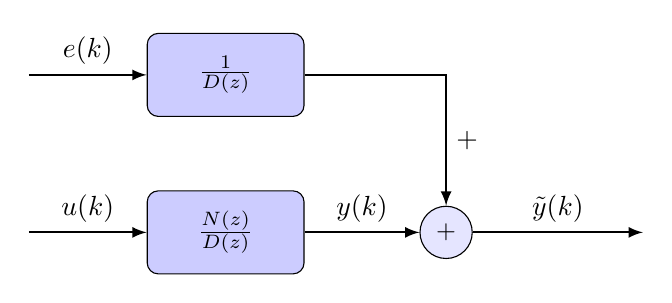
\begin{tikzpicture}[auto, node distance=2.5cm, >=latex]
    % Define styles
    \tikzstyle{block} = [rectangle, draw, fill=blue!20, 
                          text width=5em, text centered, rounded corners, minimum height=3em]
    \tikzstyle{input} = [coordinate]
    \tikzstyle{output} = [coordinate]
    \tikzstyle{sum} = [draw, fill=blue!10, circle, node distance=1.5cm]
    \tikzstyle{arrow} = [thick,->,>=latex]
    
    % Nodes
    \node [input] (input) {};
    \node [block, right of=input] (Gz) {$\frac{N(z)}{D(z)}$};
    \node [output, right of=Gz] (output) {};
    \node [block, above of=Gz, node distance=2cm] (Dz) {$\frac{1}{D(z)}$};
    \node [sum, right of=Gz, node distance=2.8cm] (sum) {\small$+$};
    \node [input, left of=Dz, node distance=2.5cm] (errorInput) {};
    \node [output, right of=sum, node distance=2.5cm] (ytilde) {};

    % Draw arrows
    \draw [arrow] (input) -- node [above] {$u(k)$} (Gz);
    \draw [arrow] (Gz) -- node [above] {$y(k)$} (sum);
    \draw [arrow] (sum) -- node [above] {$\tilde{y}(k)$} (ytilde);
    
    % Error signal and Dz block
    \draw [arrow] (errorInput) -- node [above] {$e(k)$} (Dz);
    \draw [arrow] (Dz) -| node [near end, right] {$+$} (sum);

\end{tikzpicture}
\end{center}



LS estimation is going to make sense, if and only if the sensor used for collecting data affect the collected data with a measurement noise obtained as a random, white signal \(e(k)\) that is filtered by the denominator of the system to be identified, \textbf{which does not make sense}!!!; the name of this setting is \textbf{\textit{Error-in-Equation}} setting, which does not correspond to data collection in practical situation, since the sensor does not know how to filter the noise to obtain \(e(k)\) that are probabilistically independent.\\

Our general conclusion is that Least-Square estimation should not be used when our collected via \textbf{a real experiment, EIV setting or OE setting}(OE is a subset of EIV problem, meaning that the input signal is perfectly known and the uncertainty affects output measurements dirrectly); that is, when we collect data from the experiment, even if the input is perfectly known, the output would be corrupted by additive or multiplicative noise by the data; using these data samples, LS method does not enjoy consistency property. However, Assumption 1 is satisfied and perfectly make sense when the LTI system to be identified is such that \(D(z) =  1\).\\
\[
D(z) = 1 \Rightarrow
\begin{cases}
\textcolor{red}{\fbox{\textcolor{black}{$
\text{Identification of \textbf{FIR (finite impulse response)}}
$}}}\\
\textcolor{red}{\fbox{\textcolor{black}{$\text{Identification of \textbf{static systems}}
$}}}
\end{cases}
\]
The reason is that when \(D(z) = 1\), the equation error \(e(k)\) is actually playing the role of the output measurement error \(\eta(k)\), which means i.i.d by definition, thereby satisfying also assumption 2. Now, some identification problems where both assumptions are satisfied.\\

\begin{example}[Examples that satisfies assuptions of the consistency property]
\textbf{1) A Finite-Pulse Response system} is defined in the following fashion:\\
    \(\mathbb{S}: y(k) = \theta_1 u(k) + \theta_2 u(k-1) + \cdots + \theta_n u(k-n+1)\)\\
  
Measured samples of the output have the following form:\\
\(
\begin{array}{l}
\tilde{y}(k) = y(k) + \eta(k)\\
\Rightarrow\\
\tilde{y} = \theta_1 u(k) + \theta_2 u(k-1) + \cdots + \theta_n u(k-n+1) + e(k)
\end{array}
\)\\
Where \(e(.) = \eta(.) \).\\

\textbf{2) Static Systems}: \\
\(\mathbb{S}: y(k) = f(u(k),\theta) = \theta_1 f_1(u(k)) + \theta_2 f_2(u(k)) + \cdots + \theta_n f_n(u(k))\)\\
Measured samples of the output have the following form:\\
\(
\begin{array}{l}
\tilde{y}(k) = y(k) + \eta(k)\\
\Rightarrow\\
\tilde{y} = \theta_1 f_1(u(k)) + \theta_2 f_2(u(k)) + \cdots + \theta_n f_n(u(k)) + e(k)
\end{array}
\)\\
such basis functions as polinomials or sinusoidal functions.\\
Where again, \(e(.) = \eta(.) \).\\
\end{example}
\begin{example}
Examples of functions \(f_n\) can be any set of 
In this case, the error \(e(k)\) enters the equation in an \textit{Error-in-Equation} fashion, which is required to satisfy the second assumption of the consistency property of LS.

\begin{center}
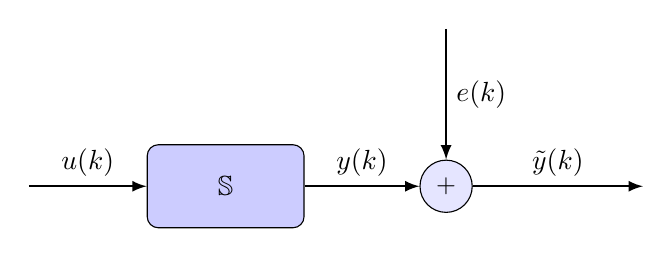
\begin{tikzpicture}[auto, node distance=2.5cm, >=latex]
    % Define styles
    \tikzstyle{block} = [rectangle, draw, fill=blue!20, 
                          text width=5em, text centered, rounded corners, minimum height=3em]
    \tikzstyle{input} = [coordinate]
    \tikzstyle{output} = [coordinate]
    \tikzstyle{sum} = [draw, fill=blue!10, circle, node distance=1.5cm]
    \tikzstyle{arrow} = [thick,->,>=latex]
    
    % Nodes
    \node [input] (input) {};
    \node [block, right of=input] (Gz) {$\mathbb{S}$};
    \node [output, right of=Gz] (output) {};
    \node [sum, right of=Gz, node distance=2.8cm] (sum) {\small$+$};
    \node [input, above of=sum, node distance=2cm] (errorInput) {};
    \node [output, right of=sum, node distance=2.5cm] (ytilde) {};

    % Draw arrows
    \draw [arrow] (input) -- node [above] {$u(k)$} (Gz);
    \draw [arrow] (Gz) -- node [above] {$y(k)$} (sum);
    \draw [arrow] (sum) -- node [above] {$\tilde{y}(k)$} (ytilde);
    
    % Error signal directly to summation point
    \draw [arrow] (errorInput) -- node [right] {$e(k)$} (sum);
\end{tikzpicture}
\end{center}
In these cases, both assumptions are satisfied, since, by assumption \(\eta\) is considered to be i.i.d, and since the error directly enters the output the first assumption is satisfied, which means:\\
\(\lim\limits_{H \to \infty} \hat{\theta}_{LS} = \theta\)\\
\end{example}

what is critical is the combination of the two assumptions, and no matter what is the structure of the system, we can always manage to define \(e(k)\) in a way that it satisfies the first assumption. The problem is that we also have to impose an additional condition, being i.i.d, on \(e(k)\) so that also the second assumption is satisfied, while based on the system equation and the way we defined \(e(k)\), this condition might not be satisfied.\\

Our next step is to reformulate this problem in a different fashion, by modifying assumption 2. In another words, it is aimed to replace assumption 2 by a "weaker assumption." This change of perspective leads to what we call \textit{Set-membership} approach to system identification.\\

\begin{QandAbox}[What about the unreachable and unobservable modes of the system?]
This is a somehow phylosophical question, which can be answered in two way:
\begin{enumerate}
\item From the practical point of view, at most engineering cases, the system that is designed does not include unobservable modes that are unstable. 
\item From a phylosophical point of view, these modes cannot be identified through input-output data collection.
\end{enumerate}
\end{QandAbox}


\chapter{Set-membership identification (discrete-time)}    % For a new chapter (works in book and report class)

Set-membership approach is an alternative to the classical, statistical identification approach. Least-Square method is one possible example of statistical estimation algorithms in the context of estimation.\\
\section{Set-membership identification of single-input-single-output LTI systems}
\subsubsection{Main ingredients}

We consider a discrete-time system described in the following parametrized regression form:\\
\begin{equation}
y(k) = f(y(k-1), y(k-2), \cdots, y(k-n), u(k), u(k-1), \cdots, u(k-m), \theta_1, \theta_2, \cdots, \theta_{n+m+1})
\end{equation}

where \(m\leq n\)\\
A-priori information on the system:
\begin{itemize}
    \item \(n\) and \(m\) are known
    \item \(f \in \mathbb{F}\) where \(\mathbb{F}\) is the class of model selected on the basis of our physical insight. 
\end{itemize}


A-priori information on the noise, the main difference with respect to the previous discussion.
\begin{itemize}
    \item the noise structure is known, i.e. the way the way uncertainty affects the input-output data)
    \item the noise is assumed to belong to konwn bounded set \(\mathbb{B}\).
\end{itemize}

When the consistency property of LS was discussed, and in general statistical approach to system identification, the typicall assumption on the noise is that statistical distribution of the noise sequence, or the value of some moments of inertia of the noise is known, such as variance. Here, the assumption is that the noise sequence \(\eta\) belongs to a bounded \(\mathbb{B}\). Remember that assumption two of the consistency property was the crucial one, so a change of perspective is adopted on the second assumption, where we deal with the following problem:

\textbf{Set-membership identification of LTI system} under the assumption that the uncertainty affecting the data can be modelled as an equation error \(e(k)\), which is exactly assumption \(1\) considered for the consistency theorem.\\
\[
\begin{aligned}
\tilde{y}(k) = & -\theta_1 \tilde{y}(k - 1) - \theta_2 \tilde{y}(k - 2) - \cdots - \tilde{y}(k - n) \\[1ex]
               & + \theta_{n+1} \tilde{u}(k) + \theta_{n+2} \tilde{u}(k - 1) + \cdots + \theta_{n+m+1} \tilde{u}(k - m) + \mathbf{e(k)} \\[2ex]
\end{aligned}
\]
where,
\[
\begin{aligned}
e(k) \in \mathbb{B}e = \left\{ \bar{e} = [e(1), e(2), \cdots, e(H)]^T \right\} : \left| e(k) \right| \leq \Delta e, \forall k
\end{aligned}
\]
where  \(\Delta e \) is a given real bounded constant.

\begin{factbox}[]
In set-membership, we always have unknown and bounded assumption about the magnitude of noise.\\

The bound is considered a conservative bound.

\end{factbox}
\subsubsection{Error-in-Variable setting}
Let's assume that the data are actually collected from a real experiment, which is EIV setup. The block-diagram representation of this a-priori information is as follows.

\begin{center}
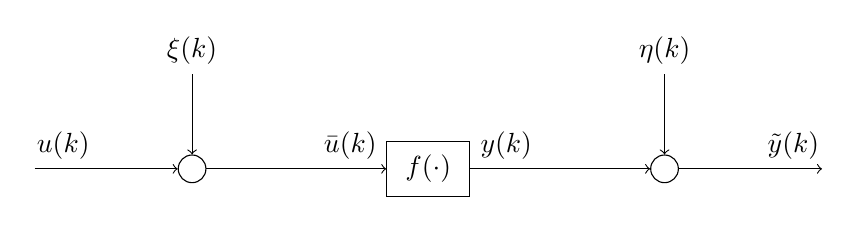
\begin{tikzpicture}[auto, node distance=2cm]

    % Block styles
    \tikzstyle{block} = [draw, rectangle, minimum height=2em, minimum width=3em]
    \tikzstyle{sum} = [draw, circle, inner sep=0pt, minimum size=1em]
    \tikzstyle{input} = [coordinate]
    \tikzstyle{output} = [coordinate]

    % Nodes
    \node [input] (input) {};
    \node [sum, right of=input, node distance=2cm] (sum1) {};
    \node [block, right of=sum1, node distance=3cm] (system) {$f(\cdot)$};
    \node [sum, right of=system, node distance=3cm] (sum2) {};
    \node [output, right of=sum2, node distance=2cm] (output) {};

    % Connections
    \draw [->] (input) -- node[pos=0.2] {$u(k)$} (sum1);
    \draw [->] (sum1) -- node[pos=0.8] {$\bar{u}(k)$} (system);
    \draw [->] (system) -- node[pos=0.2] {$y(k)$} (sum2);
    \draw [->] (sum2) -- node[pos=0.8] {$\tilde{y}(k)$} (output);
    
    % Noise terms
    \node [above of=sum1, node distance=1.5cm] (xi) {$\xi(k)$};
    \draw [->] (xi) -- (sum1);
    
    \node [above of=sum2, node distance=1.5cm] (eta) {$\eta(k)$};
    \draw [->] (eta) -- (sum2);

\end{tikzpicture}
\end{center}

\textit{Errors-in-variables} (EIV) problems refer to the most general case where both the input and the output collected samples are affected by noise.

\[
\xi = [\xi(1), \dots, \xi(H)] \in \mathcal{B}_{\xi}
\]
\[
\eta = [\eta(1), \dots, \eta(H)] \in \mathcal{B}_{\eta}
\]

$\mathcal{B}_{\xi}$ and $\mathcal{B}_{\eta}$ are bounded sets described by \textbf{\textit{polynomial constraints}.}

Most common case:
\[
\mathcal{B}_{\eta} = \left\{\eta : |\eta(k)| \leq \Delta_{\eta}\right\}, \quad \mathcal{B}_{\xi} = \left\{\xi : |\xi(k)| \leq \Delta_{\xi}\right\}
\]
Here, $f(.)$ belogn to a class of function $\mathbb{F}$, which is the a-priori assumption on the system.\\

Considering this a-priori information about the structure of the course, and a-priori information about the system, which is LTI second-order system. The noises can be reformulated as \textbf{Error-in-Equation}, which is the same as the first assumption of the consistency property of Least Square.


\[
\begin{array}{l}
\tilde{y}(k)= -\theta_1 \tilde{y}(k - 1) - \theta_2 \tilde{y}(k - 2) + \theta_3 \tilde{u}(k) + \theta_4 \tilde{u}(k - 1) + \theta_5 \tilde{u}(k - 2) \\[1ex]
\textcolor{red}{\fbox{\textcolor{black}{$+ \theta_1\eta(k-1) + \theta_2\eta(k-2) - \theta_3\xi(k) - \theta_4\xi(k-1) - \theta_5\xi(k-2) + \eta(k) $}}} =: + e(k) \\
\end{array}
\]

Up till now, nothing is changes, we now that statistically this kind of error is not i.i.d. The difference in is regarding the second assumption about the noise, \(e(k)\), which is the boundedness of the noise:

\[\left| e(k)\right| \leq \Delta e \forall k = 1, 2, ..., N\]

Provided that we find a way to compute the bound \(\Delta e \), on \(\left| e(k)\right|\), the identification problem can be correctly formulated in terms of \textbf{Equation-Error} structure in Set-membership framework. \textbf{However, Computing \(\Delta e \) is not an easy task}. Since it cannot be done without any assumption about \(\theta_i\), since they are to be identified.

\subsubsection{Set-membership formulation of the problem identifying a second order LTI system assuming an Equation-Error structure for the uncertainty}
Main ingredients:
\begin{enumerate}
\item \textbf{a-priori information }about the system, second order LTI, and the noise, Equation-Error structure and boundedness.
\item\textbf{ a-posteriori information} are experimentally collected input-output data samples.
\end{enumerate}
Now, here, we have the concept of \textit{Feasability Parameter Set}.

\subsubsection{Feasability parameter set}
The feasability parameter set \(\mathbb{D}_\theta\) is the set of all the values of the parameter vector \(\theta = \left[ \theta_1 \theta_2 \cdots \theta_p \right]^T \in \mathbb{R}^p\), which are consistent with all the avialable information on the system and the noise, and all he collected data.\\
To better understand the meaning of FPS, \(\mathbb{D}_\theta\), let's assume that we are collecting data according to the following\textbf{ Output-Error} setup:\\

\begin{center}    % Block styles
\begin{tikzpicture}[auto, node distance=2cm]

    \tikzstyle{block} = [draw, rectangle, minimum height=2em, minimum width=3em]
    \tikzstyle{sum} = [draw, circle, inner sep=0pt, minimum size=1em]
    \tikzstyle{input} = [coordinate]
    \tikzstyle{output} = [coordinate]

    % Nodes
    \node [input] (input) {};
    \node [block, right of=input, node distance=3cm] (system) {$f(\cdot)$};
    \node [sum, right of=system, node distance=3cm] (sum2) {};
    \node [output, right of=sum2, node distance=2cm] (output) {};

    % Connections
    \draw [->] (input) -- node[pos=0.5] {$u(k)$} (system);
    \draw [->] (system) -- node[pos=0.2] {$y(k)$} (sum2);
    \draw [->] (sum2) -- node[pos=0.8] {$\tilde{y}(k)$} (output);
    
    % Noise terms at the output
    \node [above of=sum2, node distance=1.5cm] (eta) {$\eta(k)$};
    \draw [->] (eta) -- (sum2);
\end{tikzpicture}
\end{center}\vspace{1cm}


Since, we have the following form of noise:\\
\[y(k) = \tilde{y} - \eta(k)\]
and we know that \(\eta\) is bounded. we can obtain the following relationship about the \(y(k)\), being that the real \(y(.)\) signal is enveloped in the following fashion:\\
\[
\tilde{y}(k) - \eta{k} \leq y(k) \leq \tilde{y}(k) + \eta{k}
\]

\begin{figure}[htbp]  % "h" for here, "t" for top, "b" for bottom, "p" for float page
    \centering
    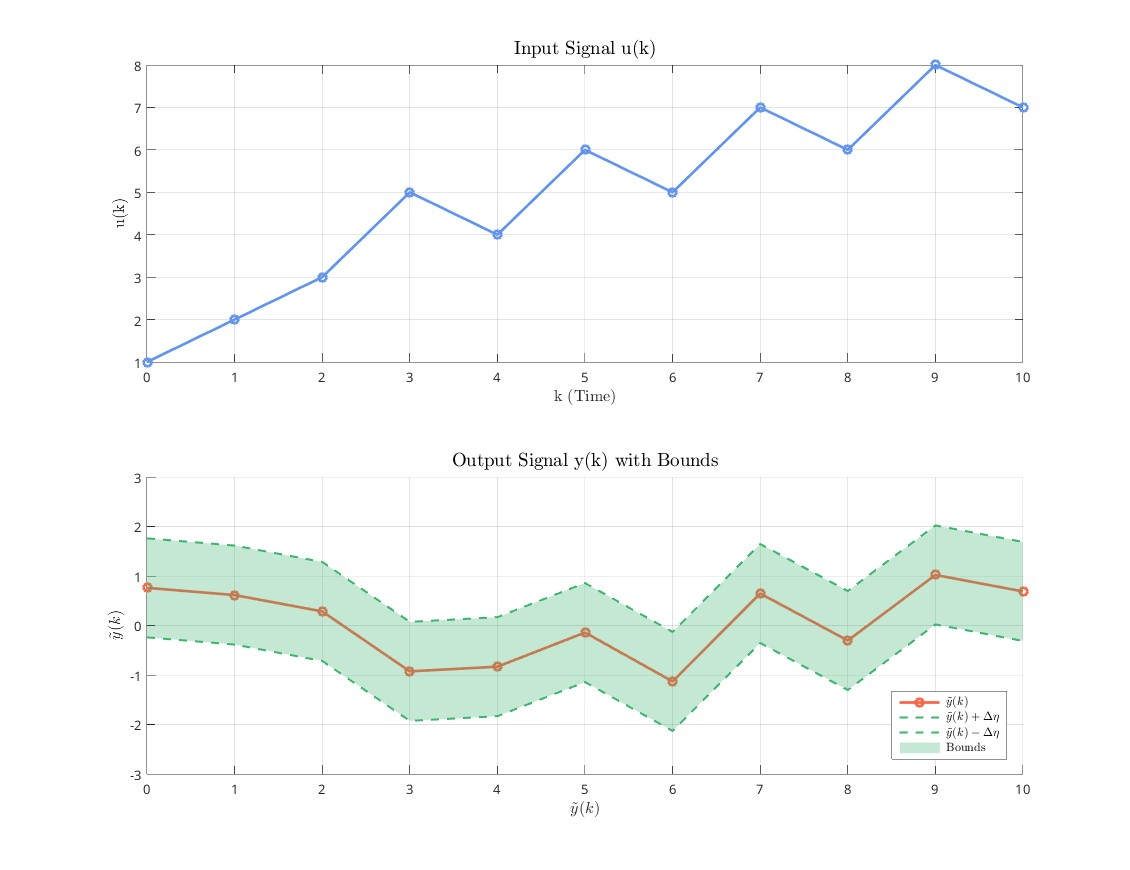
\includegraphics[width=0.75\textwidth]{images/FPS_time_domain.jpg}
    \caption{The bounds for \(y\) encompass all the elements of the \(\theta\) vector, leading to a relation for \(y\) such that its graph is bounded between the represented bounds.}
    \label{fig:FPS_time_domain}
\end{figure}

\begin{factbox}[Professor's Quotes]
In the statistical identification, assuming probabilistic characteristics for the noise, instead of having bounded interval around each single sample of the output that we collect, we have a normal distribution around each single point. Therefore, a correct formulation of the identification, again, in that context, lead to a set of models, but this time instead of having a bounded set of possible models solving the problem, we obtain a set that is statistically described, where each models have a certain probability of being the correct model.
\end{factbox}

Now, let's try to define mathematically, the FPS \(\mathbb{D}_\theta\)
\[
\begin{aligned}
\mathbb{D}_\theta = \{
\theta = \left[\theta_1 \, \theta_2 \, \cdots \, \theta_p \right]^T \in \mathbb{R}^p \, | \, 
\tilde{y}(k) = & -\theta_1 \tilde{y}(k - 1) - \theta_2 \tilde{y}(k - 2) + \theta_3 \tilde{u}(k) + \theta_4 \tilde{u}(k - 1) \\
& + \theta_5 \tilde{u}(k - 2) + e(k) \, | \, \forall k > 3 \,,\, |e(k)|\leq \Delta e
\}
\end{aligned}
\]
However, this mathematical description is not correct, since here we define FPS as a subset of \textbf{parameter space}, \(\mathbb{R}^p\), but the description of the unknown error is not in the parameter space. How can we reformulate? Although we don't know \(e\), we know that this unknown error is bounded by \(\Delta e\), so how can we exploit this information?

\[
\begin{array}{l}
\mathbb{D}_\theta = \{
\theta \in \mathbb{R}^p \, | \, 
e(k) = \tilde{y}(k) + \theta_1 \tilde{y}(k - 1) + \theta_2 \tilde{y}(k - 2) 
- \theta_3 \tilde{u}(k) - \theta_4 \tilde{u}(k - 1) - \theta_5 \tilde{u}(k - 2), \\
\forall k > 3 \,,\, |e(k)| \leq \Delta e
\}
\end{array}
\]
\[
\Rightarrow
\begin{array}{l}
\mathbb{D}_\theta = \{
\theta \in \mathbb{R}^p \, : \, 
|\tilde{y}(k) + \theta_1 \tilde{y}(k - 1) + \theta_2 \tilde{y}(k - 2) 
- \theta_3 \tilde{u}(k) - \theta_4 \tilde{u}(k - 1) - \theta_5 \tilde{u}(k - 2)|\leq \Delta e, \\ \forall k > 3
\}
\end{array}
\]
Now, we have obtained \textbf{an implicit description} of the set of \textbf{all the feasible solutions to our identification problem}, in terms of a set of inquality constraints only involving \(\theta\). \(\mathbb{D}_\theta\) is now clearly a subset of the parameter space \(\mathbb{R}^p\).

Graphical representation of \(\mathbb{D}_\theta\) in a two-dimensional space case is something of this kind:

\begin{figure}[htbp]  % "h" for here, "t" for top, "b" for bottom, "p" for float page
    \centering
    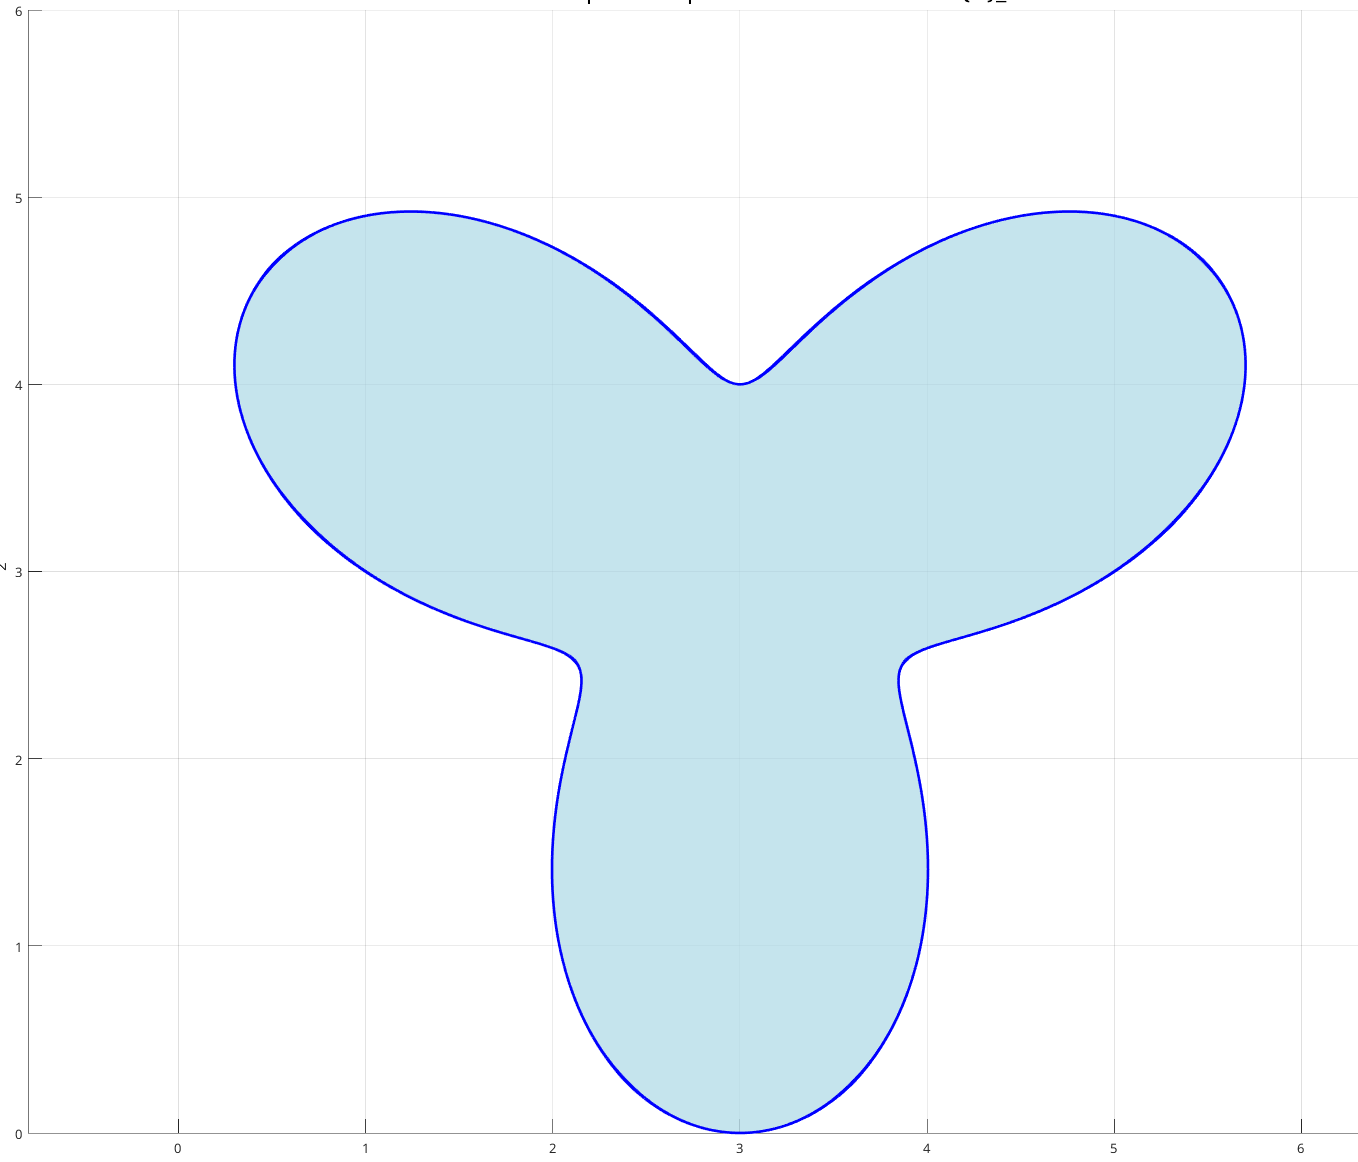
\includegraphics[width=0.65\textwidth]{images/2d-fps.png}
    \caption{a generic two-dimensional FPS}
    \label{fig:2d-fps}
\end{figure}

\subsubsection{Main features of \(\mathbb{D}_\theta\) to be discussed:}


\begin{enumerate}[label=\Roman*.] % Use label=\Roman* for Roman numerals
    \item \textbf{Boundedness of \(\mathbb{D}_\theta\)}
    \item \textbf{Usefulness of \(\mathbb{D}_\theta\)}: What is the relationship between \(\mathbb{D}_\theta\) and \(\theta\), the real value of the parameters.
\end{enumerate}

\textbf{The answer to II: }\\
Assuming that the a-priori assumption about the system and about the noise are correct. then, \(\theta\), the true parameter vector, belong to the set \(\mathbb{D}_\theta\) .

\textbf{The answer to I: }\\
The boundedness of \(\mathbb{D}_\theta\) depends on the way the data is collected. For the moment, let's assume that \(\mathbb{D}_\theta\) is bounded. 

Now that we have obtained an implicit description of \(\mathbb{D}_\theta\), how can a useful model from \(\mathbb{D}_\theta\) can be extracted, e.g. to simulate the behavior of the system under the study or to design a controller for such a system?

We consider two class of SM estimation algorithms, or estimators: 
\begin{enumerate}
\item \textbf{Set-valued estimator:} defined as \textbf{an} estimation algorithm that \textbf{provides a} possibly conservative \textbf{description} of \(\mathbb{D}_\theta\) in \textbf{a simplified geometric form} that can be easily used to simulate or control the system.
\item \textbf{Pointwise estimators:} defined as estimation algorithms that provide a single value of \(\hat{\theta}\), which is an optimal estimate of \(\theta\) \textbf{in some sense to be defined.}
\end{enumerate}

Among all possible estimators in the class \textit{1}, we consider the algorithm that provides the minimum volume box outer bounding \(\mathbb{D}_\theta\).\\

\begin{figure}[htbp]  % "h" for here, "t" for top, "b" for bottom, "p" for float page
    \centering
    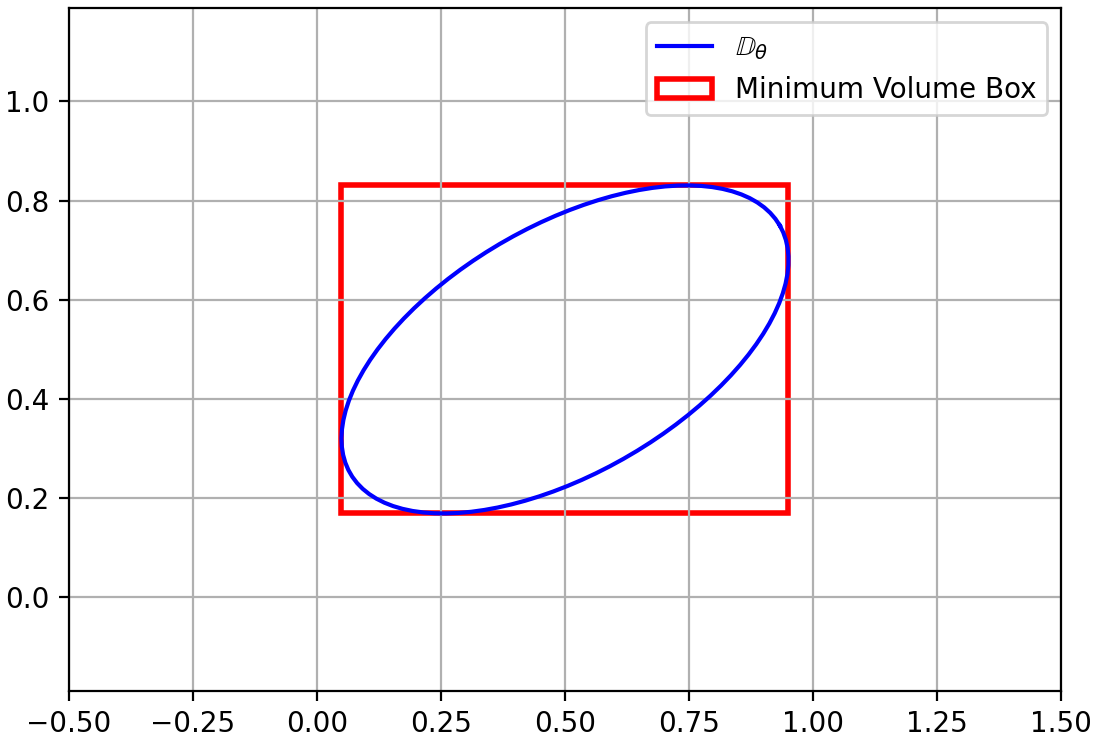
\includegraphics[width=0.65\textwidth]{images/pui.png}
    \caption{Parameter Uncertainty Intervals, considering the first case mentioned above.}
    \label{fig:PUI}
\end{figure}


This estimator is implicitly providing what we will call \textit{Parameter Uncertainty Intervals}, \textbf{PUI}s defined as bellow: 
\[
PUI_{\theta_J} = \left[\: \underline{\theta_J}, \overline{\theta_J} \: \right]
\]
where: 
\[
\underline{\theta_J} := \min\limits_{\mathbb{D}_\theta} \theta_J
\]
and
\[
\overline{\theta_J} := \max\limits_{\mathbb{D}_\theta} \theta_J = \min\limits_{\mathbb{D}_\theta} (-\theta_J)
\]

Since we know for sure, the true value of the parameter is inside the outerbox, we know that each PUI includes the true value of a parameter.\\

\begin{figure}[htbp]  % "h" for here, "t" for top, "b" for bottom, "p" for float page
    \centering
    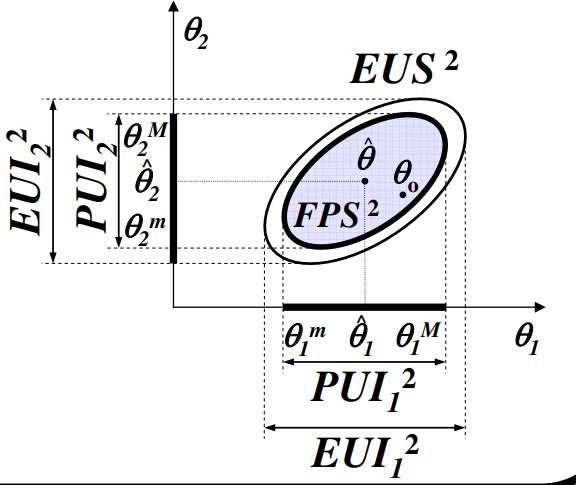
\includegraphics[width=0.4\textwidth]{images/pui2.png}
    \caption{Parameter Uncertainty Intervals, considering the first case mentioned above.}
    \label{fig:PUI}
\end{figure}
\newpage

\subsubsection{Designing a controller for a system described in this manner}
For instance, consider the following system:\\
\[
G(s) = \frac{\theta_2}{s + \theta_1}
\text{ such that: }
\begin{cases}
\theta_1 \in \left[\underline{\theta_1}, \, \overline{\theta_1} \right] \\
\theta_2 \in \left[\underline{\theta_2}, \, \overline{\theta_2} \right]
\end{cases}
\]
The Bode plot of such a transfer function is a range which can be seen in figure \ref{fig:bode_PUI}.\\

Assuming that you want to design a lead/lag controller in the frequency-domain. We need to consider the Nichol plot which is farthers from -180 and the design procedure is done. In this way after the design, rest assured, all the possible transfer functions would satisfy the requirements.

\begin{figure}[htbp]  % "h" for here, "t" for top, "b" for bottom, "p" for float page
    \centering
    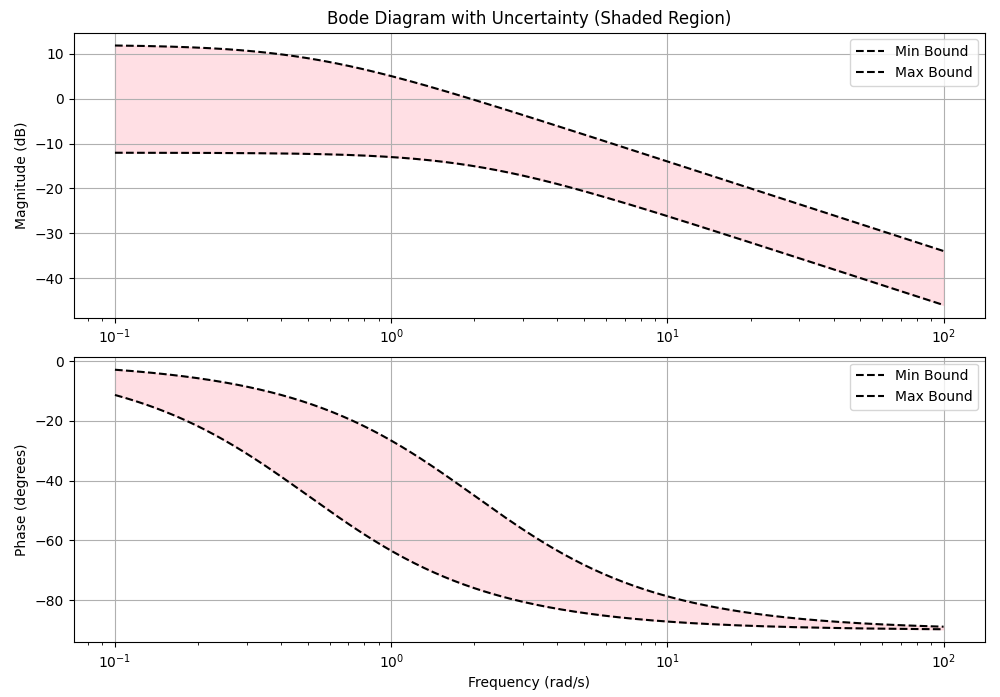
\includegraphics[width=0.7\textwidth]{images/bode_PUI.png}
    \caption{The envelop of all a transfer functions described in such a manner with uncertainties on the parameters.}
    \label{fig:bode_PUI}
\end{figure}


\subsubsection{What are the geometrical features of \(\mathbb{D}_theta\) for the specific case when the system is LTI and the uncertanty affects the data can be described by means of a bounded equation error?}
For example, consider the following assumption regarding a-priori information about the system dynamics.
\[
\begin{array}{l}
G(z) = \frac{\theta_2 z}{z + \theta_1} \\ [2ex]
\Rightarrow 
G(q^{-1}) = \frac{\theta_2}{1 + \theta_2 q^{-1}} \\ [2ex]
\Rightarrow 
y(k) = \frac{\theta_2}{1 + \theta_1 q^{-1}} u(k) \\ [2ex]
\Rightarrow 
y(k) + \theta_1 y(k-1) = \theta_2 u(k) \\[2ex]
\Rightarrow
y(k) = -\theta_1y(k-1) +\theta_2 u(k)
\end{array}
\]
A-priori information about the noise is:
\begin{itemize}
    \item Equation Error, \(e(k)\), affects the system.
    \item \(e(k)\) is bounded by a norm, \(|e(k)| < \Delta e\).
\end{itemize}

A-posteriori information are the collected samples of \(\tilde{u}(k), \, \tilde{y}(k)\).\\

Based on the informations at hand:
\[
\begin{array}{c}
\mathbb{D}_\theta = 
\left\{
\theta \in \mathbb{R}^2 : \tilde{y}(k) = - \theta_1\tilde{y}(k-1) + \theta_2 \tilde{u}(k) + e(k), \, |e(k)|<\Delta e \:\: \forall k= 1,2,\cdots,N 
\right\}\\[2ex]
\Rightarrow
\mathbb{D}_\theta = 
\left\{
\theta \in \mathbb{R}^2 : |\tilde{y}(k) + \theta_1\tilde{y}(k-1) - \theta_2 \tilde{u}(k) |<\Delta e \:\: \forall k= 2,\cdots,N 
\right\}\\[2ex]
\Rightarrow
\mathbb{D}_\theta = 
\left\{
\theta \in \mathbb{R}^2 : -\Delta e < \tilde{y}(k) + \theta_1\tilde{y}(k-1) - \theta_2 \tilde{u}(k) ,\:\:  \tilde{y}(k) + \theta_1\tilde{y}(k-1) - \theta_2 \tilde{u}(k) <\Delta e \:\: \forall k>2
\right\}\\[2ex]
\end{array}
\]
Therefore, for \(k=2\) two constraints are obtained on FPS, leading to the regione between two parallel line. 
\[
-\Delta e <\tilde{y}(k) + \theta_1\tilde{y}(k-1) - \theta_2 \tilde{u}(k) \Rightarrow
\theta_2\geq \frac{\tilde{y}(1)}{\tilde{u}(2)} + \frac{\tilde{y}(2) - \Delta e}{\tilde{u}(2)}
\]
Which leads to the following region in the parameter space:\\
THE PLOT TO BE PLOTTED.\\

Here, from the other inequality we obtain the second constraint.\\
\[
\tilde{y}(k) + \theta_1\tilde{y}(k-1) - \theta_2 \tilde{u}(k) <\Delta e \Rightarrow
\theta_2\leq \frac{\tilde{y}(1)}{\tilde{u}(2)} + \frac{\tilde{y}(2) + \Delta e}{\tilde{u}(2)}
\]

THE PLOT TO BE PLOTTED.\\

Exploiting \textit{a-priori} information and two input-output samples, one can obtain an unbounded set for $\mathbb{D}_\theta$. It is evident that, even in the noise-free case, three data samples are needed to solve the system of equations to obtain the true values of the parameters: the order of the system plus the number of parameters. 

For $k = 3$, we obtain two additional constraints, which lead to two parallel lines in the parameter space. This results in a bounded \textbf{Feasible Parameter Set (FPS)} $\mathbb{D}_\theta$. \textbf{Therefore, by our weak assumptions and with three data samples, we have obtained a bounded set as the \textit{Feasible Parameter Set}.}

\begin{factbox}
If the \textit{a-priori} assumptions are correct, the existence of an FPS is guaranteed. However, if the assumptions are not satisfied—either because the system is nonlinear and not LTI, its order is different, or the magnitude of the noise is larger than assumed—the FPS will become a \textbf{null set}. This, in itself, is a positive feature of this method, providing feedback about our estimation. Nonetheless, the statistical method does not enjoy such a property. That is, regardless of the situation, the Least Squares (LS) algorithm will provide an estimation that may not appropriately describe the system.
\end{factbox}

In general, we can conclude that under the considered assumption (LTI system with bounded equation error) the FPS, \(\mathbb{D}_\theta\), is a \textbf{polytope}, and therefore, the PUIs can be numerically computed by solving a set of \textit{linear programming} (LP) problems. \\
\begin{example}[example]
\[
\text{PUI}_{\theta_1} = \left[\underline{\theta_1}, \, \overline{\theta_1}\right]
\]
Considering our LTI system:
\[
\theta_1 = \min\limits_{\theta \in \mathbb{D}_\theta} \theta_1 = \min\limits_{\theta \in \mathbb{R}^n} \theta_1 \text{ subject to }\{ 
\begin{array}{l}
\tilde{y}(k) + \theta_1 \tilde{y}(k-1) - \theta_2 \tilde{u}(k) < \Delta e \\[1ex]
-\tilde{y}(k) - \theta_1 \tilde{y}(k-1) + \theta_2 \tilde{u}(k) < \Delta e
\end{array}\}
\]
In order to obtain the upper bound of \( PUI_{\theta_1} \), it is enough to do minimization for \(-\theta_1\).
\[
\theta_2 = \min\limits_{\theta_1 \in \mathbb{R}^n} -\theta_1 \text{ subject to } \{ 
\begin{array}{l}
\tilde{y}(k) + \theta_1 \tilde{y}(k-1) - \theta_2 \tilde{u}(k) < \Delta e \\[1ex]
-\tilde{y}(k) - \theta_1 \tilde{y}(k-1) + \theta_2 \tilde{u}(k) < \Delta e
\end{array}
\}
\]

\end{example}
A general LP problem is as follows:\\

\[
\min \limits_{x \in \mathbb{R}^n} C^Tx \text{ subject to } Ax\preceq b 
\]

We say that an optimization problem is an LP problem if the problem can be exactly written as the minimization of a linear combination of optimization variable \(x\) subject to a set of linear inequalitiies and/or equalities.\\

LP problems are convex, or at any rate linear, optimization problems that can be solved to the global optimial solution in MATLAB by using the function \textit{\textbf{linprog}}. Therefore, all the time that we have a system with a dynamic that is linear with respect to the parameters, and that we have a bounded noise, we can reach the solve a linear optimization problem.
\begin{QandAbox}
Considering \textbf{the second problem of the first lab}, which asks for the solution of the optimal \(l_\infty\) estimation problem, we consider the same setting used for the first problem, but we look for the following estimation:\\
\[
\hat{\theta}_{l_\infty} = \arg \min\limits_{\theta \in \mathbb{R}^n}\|\bar{y} - A\theta\|_\infty
\]

where \(\|.\|_\infty\) is the \(l_\infty\) norm of a vector.

\textbf{Hint for solving the problem:}\\
\[
\hat{\theta}_{l_\infty} = \arg \max\limits_{\theta \in \mathbb{R}^n}(|\rho(1)|,\, |\rho(2)|,\, \cdots,\, |\rho(N-m)|)
\]
Can this problem be written as an LP problem? the answer is yes and we have to do it to solve the second problem.
\end{QandAbox}

\subsubsection{Set-membership estimation with EIV set-up}
Now, it is aimed to consider a situation which is must more realistic with respect to the previous problem that was dealt with.\\
Previously, we discussed that, even if the noise affects the measurements in the real data acquisition setting in an EIV setting, we can reformulate EIV in an equation error. Nonetheless, we faced a major problem, which is the fact that the error $e(k)$ added to the equation is no more i.i.d.. In set-membership approach being discussed, this is no more a problem as long as it is guaranteed that the norm of this error is going to be bounded; here, there is no assumption on the statistical characteristic of this noise. Now, the problem is that computing a bound for the norm of the error is not an easy task, since after the reformulation of the problem the error norm involve yet-to-be-estimated parameters. Therefore, practically, it is difficult, if not impossible, to compute a bound on the noise, even if the bound of the noise affecting the measurements is known. This is suggesting us that maybe it is better to formulate the problem in another way, not in equation-error, but in EIV setting in a different formulation.

\begin{center}
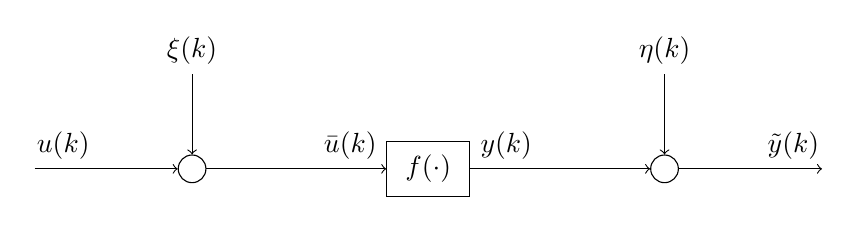
\begin{tikzpicture}[auto, node distance=2cm]

    % Block styles
    \tikzstyle{block} = [draw, rectangle, minimum height=2em, minimum width=3em]
    \tikzstyle{sum} = [draw, circle, inner sep=0pt, minimum size=1em]
    \tikzstyle{input} = [coordinate]
    \tikzstyle{output} = [coordinate]

    % Nodes
    \node [input] (input) {};
    \node [sum, right of=input, node distance=2cm] (sum1) {};
    \node [block, right of=sum1, node distance=3cm] (system) {$f(\cdot)$};
    \node [sum, right of=system, node distance=3cm] (sum2) {};
    \node [output, right of=sum2, node distance=2cm] (output) {};

    % Connections
    \draw [->] (input) -- node[pos=0.2] {$u(k)$} (sum1);
    \draw [->] (sum1) -- node[pos=0.8] {$\bar{u}(k)$} (system);
    \draw [->] (system) -- node[pos=0.2] {$y(k)$} (sum2);
    \draw [->] (sum2) -- node[pos=0.8] {$\tilde{y}(k)$} (output);
    
    % Noise terms
    \node [above of=sum1, node distance=1.5cm] (xi) {$\xi(k)$};
    \draw [->] (xi) -- (sum1);
    
    \node [above of=sum2, node distance=1.5cm] (eta) {$\eta(k)$};
    \draw [->] (eta) -- (sum2);

\end{tikzpicture}
\end{center}

\textit{Errors-in-variables} (EIV) problems refer to the most general case where both the input and the output collected samples are affected by noise.

\[
\xi = [\xi(1), \dots, \xi(H)] \in \mathcal{B}_{\xi}
\]
\[
\eta = [\eta(1), \dots, \eta(H)] \in \mathcal{B}_{\eta}
\]

$\mathcal{B}_{\xi}$ and $\mathcal{B}_{\eta}$ are bounded sets described by \textbf{\textit{polynomial constraints}.}

Most common case:
\[
\mathcal{B}_{\eta} = \left\{\eta : |\eta(k)| \leq \Delta_{\eta}\right\}, \quad \mathcal{B}_{\xi} = \left\{\xi : |\xi(k)| \leq \Delta_{\xi}\right\}
\]
which is a hyper-dimensional box.

A subset of this problem, as was discussed also in the previous chapter, is Output-Error, OE, set-up, meaning that the input signal is perfectly known.


\begin{center}    % Block styles
\begin{tikzpicture}[auto, node distance=2cm]

    \tikzstyle{block} = [draw, rectangle, minimum height=2em, minimum width=3em]
    \tikzstyle{sum} = [draw, circle, inner sep=0pt, minimum size=1em]
    \tikzstyle{input} = [coordinate]
    \tikzstyle{output} = [coordinate]

    % Nodes
    \node [input] (input) {};
    \node [block, right of=input, node distance=3cm] (system) {$f(\cdot)$};
    \node [sum, right of=system, node distance=3cm] (sum2) {};
    \node [output, right of=sum2, node distance=2cm] (output) {};

    % Connections
    \draw [->] (input) -- node[pos=0.5] {$u(k)$} (system);
    \draw [->] (system) -- node[pos=0.2] {$y(k)$} (sum2);
    \draw [->] (sum2) -- node[pos=0.8] {$\tilde{y}(k)$} (output);
    
    % Noise terms at the output
    \node [above of=sum2, node distance=1.5cm] (eta) {$\eta(k)$};
    \draw [->] (eta) -- (sum2);
\end{tikzpicture}
\end{center}\vspace{1cm}
where,
\begin{itemize}
\item 
\[
\eta = \left[\eta(1),\,\eta(2),\, \cdots,\,\eta(H)\right] \in \mathbb{B}_\eta
\]
\item \(\mathbb{B}_\eta\) is a bounded set described by \textbf{\textit{polynomial constraints}}.
\item Most common case: \(\mathbb{B}_\eta = \left\{\eta: \: |\eta(k)| \leq \Delta_\eta \right\}\)
\end{itemize}

The FPS for the general EIV problem is implicitly defined as follows:
\[
\begin{array}{c}
\mathbb{D}_\theta = \{ \theta \in \mathbb{R}^n : \, y(k) = f( y(k-1), y(k-2), \cdots, y(k-n),  u(k), u(k-1), \cdots \\[1ex]
, u(k-m), \theta_1, \theta_2, \cdots, \theta_{n+m+1}),k = n+1,\,n+2,\,\cdots,\,N,\: y(k) = \tilde{y}(k) - \eta(k), \\[1ex]
u(k) = \tilde{u}(k) - \xi(k),\: k=1,\,2,\,\cdots,\,N,\: |\xi(k)|\leq \Delta\xi(k),\: |\eta(k)\leq \Delta\eta(k),\: k = 1,\,2,\,\cdots,\,N \}
\end{array}
\]

The FPS for the case of \textbf{LTI descrete-time systems with EIV noise structure} is given by:
\[
\mathbb{D}_\theta = \left\{ \theta \in \mathbb{R}^p : \, (\tilde{y}(k) - \eta(k)) + \sum_{i=1}^{n} a_i (\tilde{y}(k - i) - \eta(k - i)) = \sum_{j=0}^{m} b_j (\tilde{u}(k - j) - \xi(k - j)), \right.
\]
\[
\left. t = n + 1, \dots, H, \quad |\xi(k)| \leq \Delta\xi(k), \quad |\eta(k)| \leq \Delta\eta(k), \quad k = 1, \dots, H \right\}
\]
This includes \(2N\) new variables involved in the FPS which are not variables in parameter space. Now, these variables should be eliminated, and this is not possible without setting some conservative conditions. \textbf{If you come up with an idea to do so without considering conservative conditions, you can publish a paper}. 

Since the FPS defined in the above equation depends on some additional unknownes( all the samples of the noise sequences). The constraints defining \(\mathbb{D}_\theta\) cannot be rearranged in such a way to eliminate dependancies on such additional variables. To solve the problem, we need to extend the space of decision variables in by defining the \textit{Extended Feasible Parameter Set}(EFPS).

\[
\begin{array}{c}
\mathcal{D}_{\theta,\eta,\xi} = \left\{ \theta \in \mathbb{R}^p, \eta \in \mathbb{R}^H, \xi \in \mathbb{R}^H : \right.
(y(k) - \eta(k) + \sum_{i=1}^{n} a_i ( y(k-i) - \eta(k-i)) = \\[2ex]
\sum_{j=0}^{m} b_j ( u(k-j) - \xi(k-j) ), \, t = n+1,\dots,H, \\[2ex]
|\xi(k)| \leq \Delta \xi(k), \, |\eta(k)| \leq \Delta \eta(k), \, k = 1,\dots,H \left.\right\}
\end{array}
\]
As you can see in the box below, here, we are expanding the space we are considering for FPS, hence EFPS.
\begin{align}
\fcolorbox{red}{white}{$\mathcal{D}_{\theta,\eta,\xi} = \left\{ \theta \in \mathbb{R}^p, \eta \in \mathbb{R}^H, \xi \in \mathbb{R}^H\right\}$}
\end{align}
A simplified graphical version is shown in the following graph. \textbf{Now, the FPS is the projection of the EFPS on the parameter space}.

\begin{figure}[htbp]  % "h" for here, "t" for top, "b" for bottom, "p" for float page
    \centering
    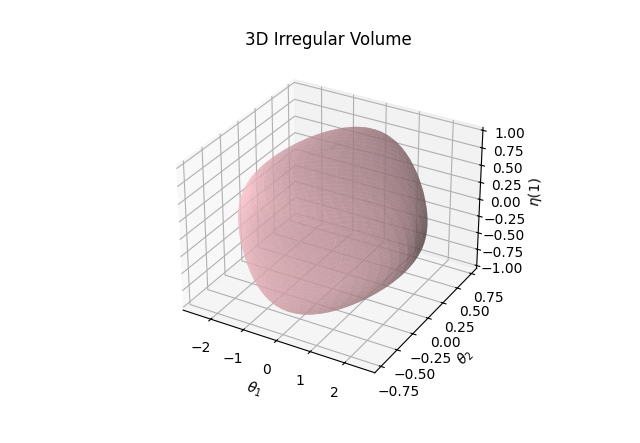
\includegraphics[width=0.7\textwidth]{images/EFPS.png}
    \caption{A simplified, general graph of EFPS.}
    \label{fig:EFPS}
\end{figure}

In this case,
\[
\underline{\theta}_k = \min\limits_{\theta \in \mathbb{D}_\theta} \theta_k = \min\limits_{\theta, \eta, \xi \in \mathbb{D}_{\theta, \eta, \xi}} \theta_k
\]
That is,
\[
\begin{array}{rcl}
\theta_k & = & \min_{\theta \in \mathbb{D}_{\theta, \eta, \xi}} \theta_k \text{ subject to } \tilde{y}(k) - \eta(k) + \sum_{i=1}^{n} \theta_i(\tilde{y}(k-i) - \eta(k-i)) \\[1ex]
& & + \theta_{n+1}(\tilde{u}(k) - \xi(k)) + \sum_{j=1}^{m} \theta_{n+j+1}(\tilde{y}(k-j) - \xi(k-j)), \\[1ex]
& & \quad \forall k > n+1, \, |\xi(k)| \leq \Delta \xi, \, |\eta(k)| \leq \Delta \eta, \, \forall k
\end{array}
\]

The drawback is that EFPS is a non-convex set defined by \textbf{polynomial} (\textit{bilinear}) constraints.

\begin{factbox}[Professor's Quote:]
To the best of my knowledge, in the domain of non-convex functions, the only class that can be optimized up to the global minimum is the class of non-convex functions with polynomial constraints.
\end{factbox}

\begin{QandAbox}[Boundedness of the noise]
Practically, the assumption that the noise can take any value is unreasonable. Since sensors are used for measurements and are designed to be stable and precise, it is not realistic for the noise to take on any value. For this reason, it makes sense to assume bounded noise.
\end{QandAbox}

\begin{factbox}[What signal to use as input signal?]
If the signal applied to a system is simply a \textbf{ramp} or \textbf{step} signal, after the transient period, the output will reflect the generalized DC gain of the system when it reaches steady-state. Therefore, a staircase of steps with varying amplitudes combined with a random signal may be a good choice to stimulate different modes of the system.
\end{factbox}

Refer to Lab 01, Problem 2, for least squares with \( l_\infty \)-norm.

Consider the following FPS. Due to its non-convexity, the optimizer may return a local minimum, which is not desirable.

\begin{figure}[htbp]  % "h" for here, "t" for top, "b" for bottom, "p" for float page
    \centering
    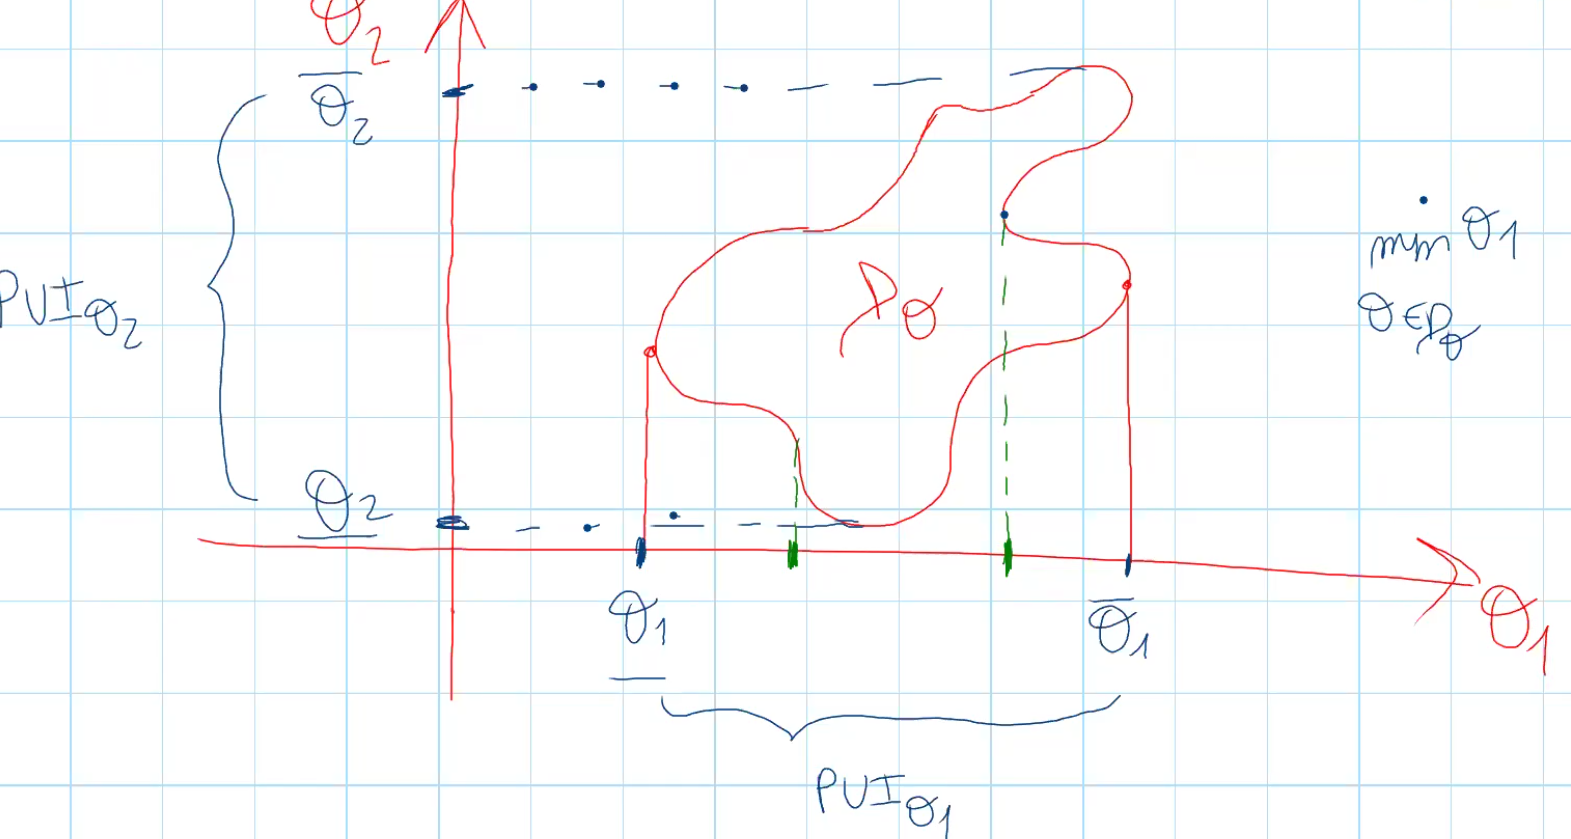
\includegraphics[width=0.7\textwidth]{images/non-convex-FPS.png}
    \caption{A simplified, general graph of EFPS.}
    \label{fig:non-convex-FPS}
\end{figure}



\subsubsection{Convext relaxation for polynomial optimization problem}
General ideas and intuitions are as follows: \\
let's consider the following general polynomial optimizatin problem:
\[
\min\limits_{x} f_0(x) \text{ s.t. } 
\begin{cases}
f_k(x) \leq 0\: (k\,=\,1,\,2,\, \cdots,\, l)\\
f_k(x) = 0\: (k\,=\,l+1,\,l+2,1,\cdots,\, m)
\end{cases}
\]
where, $f_0$ and $f_k$ are multivariable polynomials in the optimization variables$x$.

\begin{example}[Example 1]
\(
x =
\begin{bmatrix}
    x_1 \\
    x_2 \\
    x_3
\end{bmatrix}
\)\\ \\
The following is what we call \textit{Polynomial Optimization Problem} \textbf{POP}\\
\(
\min (x_1^2 + x_2x_3^3 + x_1^5x_2^3 + 7x_3^2 + \cdots)
\)\\ \\
for the second order case:
\(
f_0(x) = \theta_0 + \theta_1x_1 + \theta_2x_2 + \theta_3x_1x_3 + \theta_4x_1^2 + \theta_5x_2^2
\)\\ \\
\end{example}

\begin{example}[Example 2]
a constraint POP
\(
\min (x_1^2 + 11x_2) \text{ s. t. } 
\begin{cases}
x_1^2 - 4 = 0 \\
x_1^3 + 7x_2 - 13x_1x_2 \leq 0
\end{cases}
\)\\ \\
\end{example}

All POPs can be written in the so-called \textit{epographic} form by introducing a new "slack" variable $\gamma$.
\[
\begin{array}{ll}
    \min\limits_{x} & f_0(x) \\
    \text{s.t.} & \\
      &\\
    & f_1(x) \geq 0 \\
    & f_2(x) \geq 0 \\
    & \vdots \\
    & f_5(x) \geq 0 \\
    & f_k(x) = 0 \\
  
\end{array}
\quad \Longleftrightarrow \quad
\begin{array}{ll}
    \min\limits_{x,\,t}t &  \\
    \text{s.t.} & \\
    & f_0(x) \leq t \text{  or  } t - f_0(x) \leq 0 \\
    & f_1(x) \geq 0 \\
    & f_2(x) \geq 0 \\
    & \vdots \\
    & f_5(x) \geq 0 \\
    & f_k(x) = 0 \\
\end{array}
\]

By rewriting a generic POP in the epigraphic form, we recognize that a generic POP can be seen as the problem of minimizing a linear function over a non-convex set described by polynomial constraints. This is also true for unconstraint POP.

\[
\begin{array}{ll}
    \min\limits_{x} & f_0(x) \\
      &\\
      &\\
\end{array}
\quad \Longleftrightarrow \quad
\begin{array}{ll}
    \min\limits_{x,\,t} & t \\
    \text{s.t.} & \\
     t - f_0(x) \leq 0 \\
  
\end{array}
\]

A graphical representation of this problem is as follows:

\begin{figure}[htbp]  % "h" for here, "t" for top, "b" for bottom, "p" for float page
    \centering
    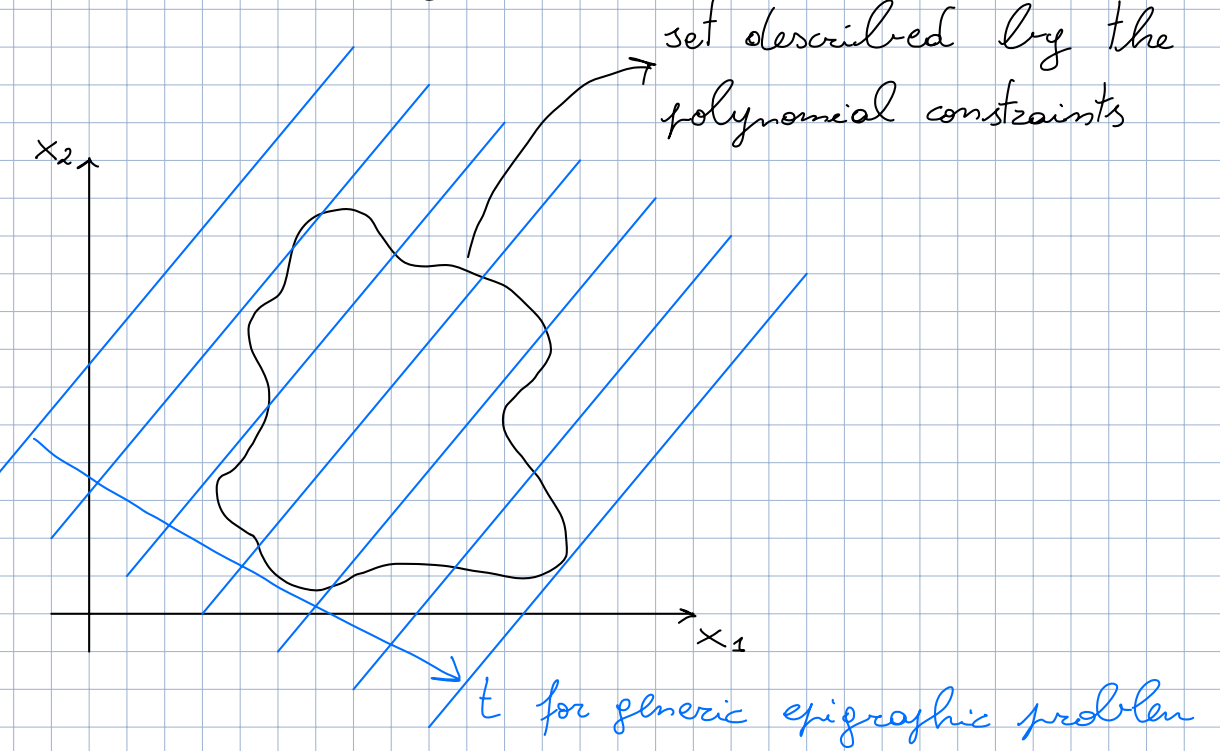
\includegraphics[width=0.7\textwidth]{images/epigraphic-mini.png}
    \caption{the geraphical representation of a generic epigraphic minization, each line represent different values of t.}
    \label{fig:non-convex-FPS}
\end{figure}

\begin{figure}[htbp]  % "h" for here, "t" for top, "b" for bottom, "p" for float page
    \centering
    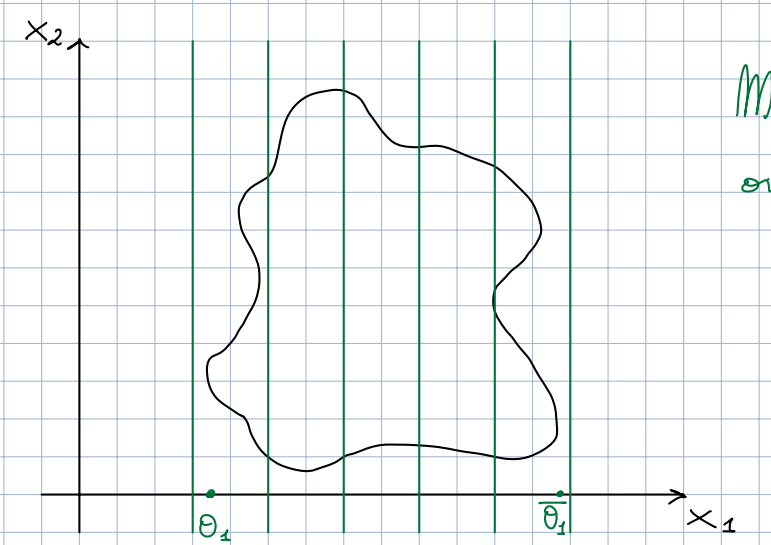
\includegraphics[width=0.65\textwidth]{images/linprog.png}
    \caption{Graphical representation of a linear programming over $\theta_1$}
    \label{fig:non-convex-FPS}
\end{figure}
\begin{QandAbox}[Important Remark]
Since a generic POP can be rewritten in the epigraphic form that is the problem of minimizing a linear function over a non-convex set, the non-convexity of the problem is now completely embedded in the description of the set of constraint.
\end{QandAbox}

If we want to be able to compute the global optimal solution to the non-convex POP, we have to deal with the non-convexity of the set of constraints.

Now, the idea is to replace the non-convex set with a convex set such that the result of the global optima is equal to that of non-convex.

\subsubsection{Convex-hull of a non-convex set}
The convex-hull of a non-convex set $S$ is
the smallest convex set that is including $S$.


\begin{figure}[htbp]  % "h" for here, "t" for top, "b" for bottom, "p" for float page
    \centering
    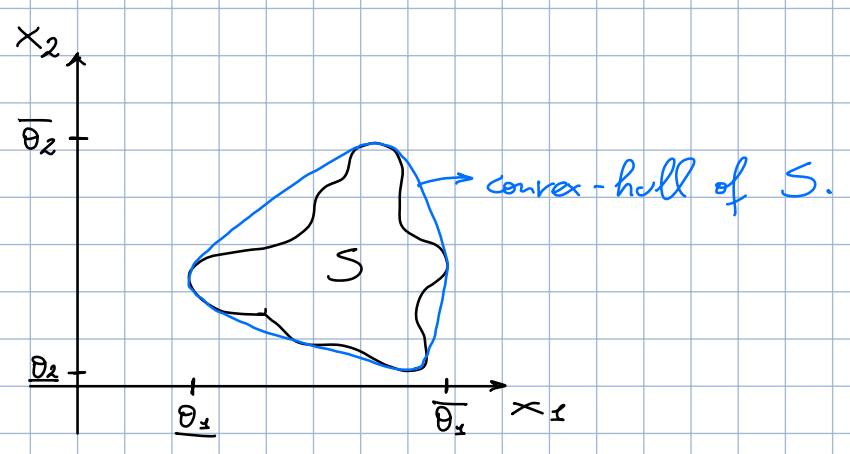
\includegraphics[width=0.65\textwidth]{images/convex-hull.png}
    \caption{convex-hull of a generic non-convex set}
    \label{fig:non-convex-FPS}
\end{figure}

The general idea here is that if we are able to write down equation describing convex-hull $C_S$ of the non-convex set $S$:
\[
\min\limits_{x \in C_s} f(x) = \min\limits_{x \in S} f(x)
\]
where $f(x)$ is a linear function of $x$.

However, in general, computing the mathematical description of the convex haul is quite a difficult problem. For the case of POPS - a particular class of non-convex optimization problem - Lassere et al were able to compute \textbf{a convex relaxation} of $S$ depending on a parameter which is called \textbf{\textit{order of relaxation $\delta$}}.

For a given fixed value of $\delta$ we have the following situation. For different order of relaxation, we obtain different convex sets including the original set. They proved by increasing the order of relaxation, we obtain convex sets that is the convex set of the original set. For the problems we are dealing with, the optimal solution is obtained with a fixed value of relaxation, and convergence is typically really fast. The issue is that the value of the $\delta$ is not known.

\begin{figure}[htbp]  % "h" for here, "t" for top, "b" for bottom, "p" for float page
    \centering
    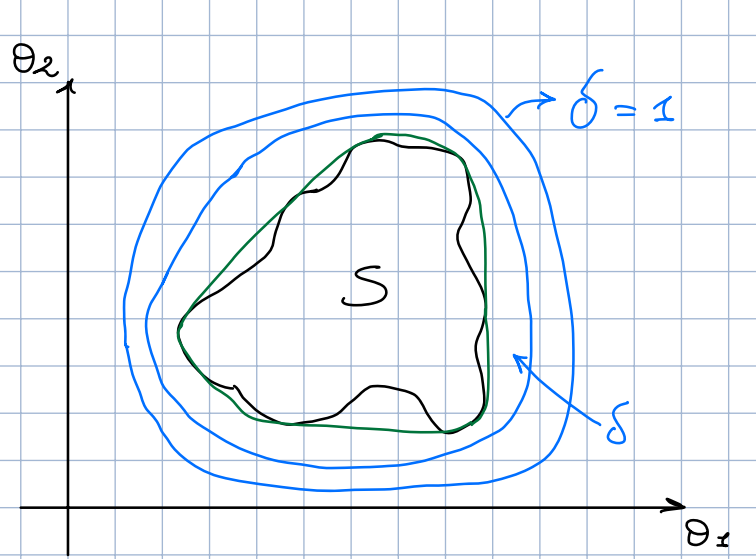
\includegraphics[width=0.65\textwidth]{images/convex-relaxation.png}
    \caption{convex-hull of a generic non-convex set}
    \label{fig:non-convex-FPS}
\end{figure}

\begin{itemize}
    \item Computation of parameter bounds (PUIs) require the solution to the global optimum of non-convex polynomial optimization problems.
    
    \item By applying \textit{Moments theory} (Lasserre) or \textit{Sum-of-squares (SOS) theory} (Chesi, Parrilo), it is possible to build a sequence of \textbf{convex} semidefinite (SDP) optimization problems whose size/complexity depends on a parameter called \textit{order of relaxation} \(\delta\).
    
    \item For any given \(\delta\), the following inequalities hold
    \[
    \theta^{\delta}_k \leq \theta_k, \quad \overline{\theta}^{\delta}_k \geq \overline{\theta}_k 
    \]
    
    \item Furthermore,
    \[
    \lim_{\delta \to \infty} \theta^{\delta}_k = \theta_k, \quad \lim_{\delta \to \infty} \overline{\theta}^{\delta}_k = \overline{\theta}_k
    \]
\end{itemize}

In gradient-based algorithms, we have the risk of underestimating the value of the parameters by trapping into local minima, while in this method, rest assured, the true value of the parameters is going to be included in the interval.

In order to solve POPs by means of Lassere convex-relaxation appraoch in MATLAB, we use the following two software, which are MATLAB toolboxes, that can be freely downloaded online:
\begin{itemize}
\item SparsePOP: given a POP and a value of the order of relaxation $\delta$, provides\textbf{ the SDP relaxed problem.}
\item Sedumi: is called by SparsePOP to solve the obtained convex SDP.
\end{itemize}

\subsubsection{The lecture after the lab 03}
In the laboratory, we saw that SparsePOP computes convex relaxation for a given relaxation. The Sediumi toolbox is used to solve the relaxed optimization problem.\\

\subsubsection{Selection of the order of relaxation}
Let's call $x^*$ the global optimal solution of a given POP, and $x^*$ the solution of the corresponding convex relaxation of order $\delta$.\\

QUESTION: How to selcet $\delta$?\\
Well, from the theory we have the following results:\\
\textbf{R1)} 
\[
\lim\limits_{\delta \to \infty} f(x^\delta) = f(x^*)
\]
which implies, the following, to be unprecise:
\[
\lim\limits_{\delta \to \infty} = x^*
\]

\textbf{R2)}: \(\delta) \geq \lceil \frac{n_{max}}{2} \rceil\), where $n_{max}$ is the maximum degree of the polynomial describing the functional and the constraints.\\

\textbf{R3)} the complexity of SDP problem obtained by applying to the original convex relaxation techniques grows exponentially in the order of relaxatoin $\delta$, as well as the number of optimization variables (AKA decision variables) of the original POP.\\

On the other hand, we have the following result too:\\

\textbf{R4)}: For a large class of problems including most of the problems in this course, it is possible to prove that the convergence to the global optimal solution of the original POP is very fast and it is achieved for a finite value of $\delta$. but still the result number 2 should be satisfied.\\

Let's analyze the impact of R1, R2, R3, and R4 on the applicationo of convex relaxation techniques to a set-membership identification problem of an LTI system with EIV assuption about the noise.\\

For SM Id. of LTI system with EIV of a polynomial of order 2, we can start with $\delta =1$. Because we have bi-linear constraints, i.e. polynomial constraints of order 2. Number of optimization variable is given by:
\[
P + 2N
\]
Where $P$ is the number of parameters to be identified and $N$ is the number of pair of data samples. Since in system identification problem $N$ is going to be quite large in many applications in order to obtain accurate PUI's, the complexity is going to be untractable. Nonetheless, the following result can be exploited:\\
\textbf{R5)} if the structure of the original POP satisfies a property called \textit{running intersection property}, it's possible to build a sequency of convex SDP relaxation, involving much less variables. (Sparse Convex - relaxation)

\begin{factbox}[about SparsePOP]
SparsePOP toolbox is able to automatically check whether the original POP satisfies the running intersection property, and if this is the case,
it applies the \textit{sparse convex relaxation}.
\end{factbox}

\textbf{R6)} The complexity of SDP problem obtained by applying the sparse convex relaxation to the original POP:
\begin{itemize}
\item\textbf{grows exponentially iwth the order of relaxation}.
\item \textbf{grows linearly with the number of optimization variables}.
\end{itemize}

\textbf{R6} tell us that the SM - ID problem for LTI system with EIV assumption is computationally tractable for a rather large value of input-output pair of experimentally collected data ($N$), since the problem satisfies the \textbf{running intersection property} and it is characterized by \textbf{bilinear constraints}, which allow us to start with relaxation $\delta =1$.

\begin{QandAbox}
considering that the problem is computationally tracktable having the constraints are bilinear. can we find a trick to solve a polynomial with large number of parameters, which may be computationally untracktable?
\end{QandAbox}

\subsubsection{How to formulate the SM - ID problem for an LTI system of order $n$ with EIV noise structrue, in terms of SparsePOP}:\\
\begin{QandAbox}[Exam matter]
The following procedure is what should be done to solve the exam problem.
\end{QandAbox}
\begin{enumerate}
\item First, let's write down the FPS and the EFPS. To simplify, here, we consider $n = 2$.\\
FPS:
\[
\begin{array}{c}
\mathbb{D}_\theta = \{\theta \in \mathbb{R}^5: y(k) + \theta_1 y(k-1) + \theta_2 y(k-2) - \theta_3 u(k) -\theta_4 u(k-1) -\theta_5 u(k-2) = 0 \\
\forall k = 3,\,4,\,\cdots,\,N, |\eta(k)\leq\Delta\eta, |\xi(k)|\leq \Delta\xi, \forall k \in \mathbb{N} 
\}
\end{array}
\]
EFPS:
\[
\begin{array}{l}
\mathbb{D}_{\theta,\,\eta,\,\xi}= \{\theta \in \mathbb{R}^5,\, \eta \in \mathbb{R}^N,\,\mathbb{R}^N
: 
\tilde{y}(k) - \eta(k)+ \theta_1 \tilde{y}(k-1) - \theta_1\eta(k-1) + \theta_2 \tilde{y}(k-2)\\-\theta_2\eta(k-2) - \theta_3 \tilde{u}(k) + \theta_3\xi(k) -\theta_4 \tilde{u}(k-1) + \theta_4\xi(k-1) -\theta_5 \tilde{u}(k-2) + \theta_5\xi(k-2) = 0 \\
\forall k = 3,\,4,\,\cdots,\,N,
|\eta(k)|\leq\Delta\eta, |\xi(k)|\leq \Delta\xi, \forall k \in \mathbb{N} 
\}
\end{array}
\]

PUI:
\[
PUI_k = \left[\underline{\theta}_k,\,\overline{\theta}_k \right]
\]
where
\[
\begin{array}{c}
\underline{\theta}_k = \min\limits_{\theta \in \mathbb{D}_\theta} \theta_k = \min\limits_{\theta, \eta, \xi \in \mathbb{D}_{\theta, \eta, \xi}} \theta_k \quad \text{s.t.} \\
\tilde{y}(k) - \eta(k) + \theta_1 \tilde{y}(k-1) - \theta_1\eta(k-1) + \theta_2 \tilde{y}(k-2) - \theta_2\eta(k-2) \\
- \theta_3 \tilde{u}(k) +\theta_3 \xi(k) - \theta_4 \tilde{u}(k-1) + \theta_4\xi(k-1) - \theta_5 \tilde{u}(k-2) + \theta_5 \xi(k-2) = 0 \quad \forall k = 3,\,4,\,\cdots,\,N,\\
\eta(k) + \Delta\eta \geq 0, \quad \Delta\eta - \eta(k) \geq 0, \quad \xi(k) + \Delta\xi \geq 0, \quad \Delta\xi - \xi(k) \geq 0 \quad \forall k \in \mathbb{N} 
\end{array}
\]

\[
\begin{array}{c}
\overline{\theta}_k = \max\limits_{\theta \in \mathbb{D}_\theta} \theta_k = \max\limits_{\theta, \eta, \xi \in \mathbb{D}_{\theta, \eta, \xi}} \theta_k \quad \text{s.t.} \\
\tilde{y}(k) - \eta(k) + \theta_1 \tilde{y}(k-1) - \theta_1\eta(k-1) + \theta_2 \tilde{y}(k-2) - \theta_2\eta(k-2) \\
- \theta_3 \tilde{u}(k) +\theta_3 \xi(k) - \theta_4 \tilde{u}(k-1) + \theta_4\xi(k-1) - \theta_5 \tilde{u}(k-2) + \theta_5 \xi(k-2) = 0 \quad \forall k = 3,\,4,\,\cdots,\,N,\\
\eta(k) + \Delta\eta \geq 0, \quad \Delta\eta - \eta(k) \geq 0, \quad \xi(k) + \Delta\xi \geq 0, \quad \Delta\xi - \xi(k) \geq 0 \quad \forall k \in \mathbb{N} 
\end{array}
\]
\item Formulating the obtained POP in terms of SparsePOP data structure.\\
Let's consider how to describe in SparsePOP terms the bilinear eqaulity constraints. Considering k = 3.
\[
\tilde{y}(3) - \eta(3) + \theta_1 \tilde{y}(2) - \eta(2) + \theta_2 \tilde{y}(1) - \eta(1) \\
- \theta_3 \tilde{u}(3) + \xi(3) - \theta_4 \tilde{u}(2) + \xi(2) - \theta_5 \tilde{u}(1) + \xi(1) = 0
\]
Now, we have to shape our data structure for this inequality.
\begin{example}
\begin{lstlisting}
ineqPolySys{c}.typeCone = -1; equality constraint
ineqPolySys{c}.dimVar = 5 + 2*N; 
% P: the number of variables involved, P = 5
% N: the number of pairs of input-output data samples
ineqPolySys{c}.degree = 2; %always 2,for bilinear equations
ineqPolySys{c}.noTerms = 12;
ineqPolySys{c}.supports = sup_matrix;
ineqPolySys{c}.coef = [y_tilde(3);-1;y_tilde(2);-1; ...]';
\end{lstlisting}
\end{example}
Support matrix show have as many row as the terms in the constraints and as many constraints as the number of optimization variables $P + 2*N$.
\newpage
\begin{figure}[htbp]  % "h" for here, "t" for top, "b" for bottom, "p" for float page
    \centering
    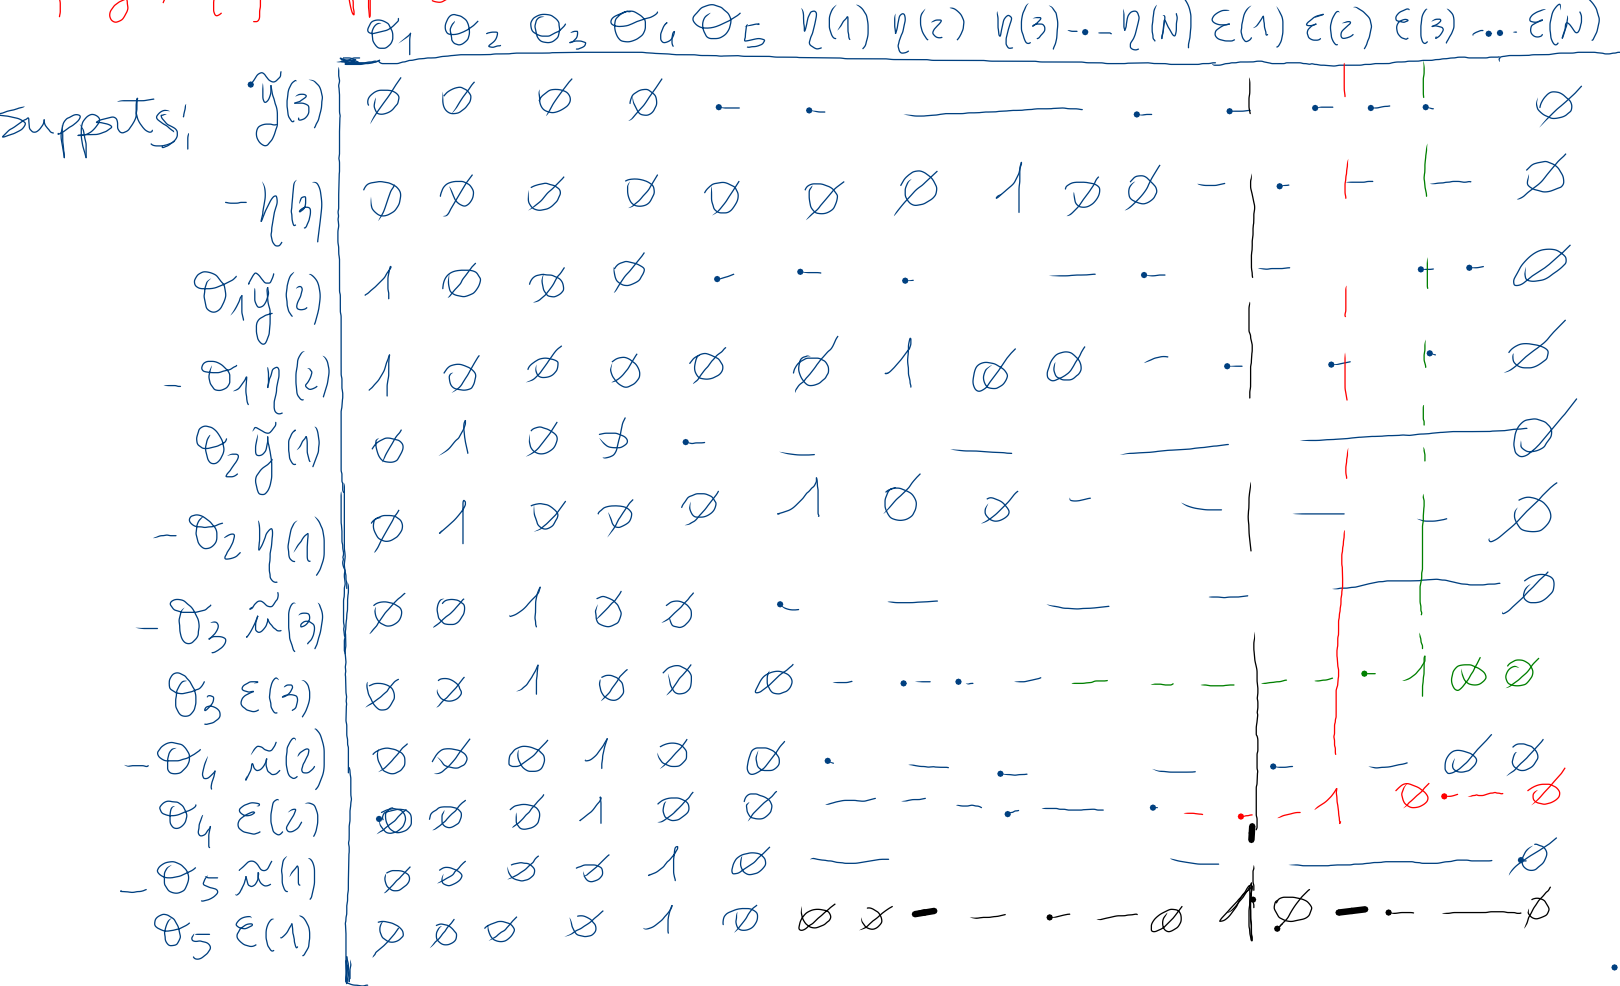
\includegraphics[width=0.75\textwidth]{images/support-matrix1.png}
    \caption{Support matrix for the equality constraints}
    \label{fig:non-convex-FPS}
\end{figure}
\end{enumerate}

Regarding the constraints on the boundedness of the noise, they can be imposed consider a lower bound and upper bound for the variables corresponding to the noise. Look at the solution of lab 03.

\newpage

\section{Set-membership identification of multi-input-multi-output LTI system}
Now that we have considered SISO LTI system, a new direction can be considering MIMO systems. Again, to formulate our problem, we should consider our a-priori and a-posteriori informations.

\subsubsection{A-priori information on the system}
The system is a MIMO LTI system with $p$ input and $q$ outputs, described by means of a \textbf{matrix transfer function} $G(q{-1})$, where the elements of it are SISO transfer function.


\[
\begin{bmatrix}
y_1 \\
y_2 \\
\vdots \\
y_q
\end{bmatrix}
=
\begin{bmatrix}
G_{11}(q^{-1}) & G_{12}(q^{-1}) & \dots & G_{1p}(q^{-1}) \\
G_{21}(q^{-1}) & G_{22}(q^{-1}) & \dots & G_{2p}(q^{-1}) \\
\vdots         & \vdots         & \ddots & \vdots         \\
G_{q1}(q^{-1}) & G_{q2}(q^{-1}) & \dots & G_{qp}(q^{-1})
\end{bmatrix}
\begin{bmatrix}
u_1 \\
u_2 \\
\vdots \\
u_p
\end{bmatrix}
\]

\begin{factbox}[Discussion about the structure this matrix transfer function]
In general, The denuminator of these transfer functions can be different, but considering that the transfer function can be obtained from steady-state representation of the system, $C*(sI-A)^{-1}B + D$, before the possible cancellations, The denuminator of all of these transfer functions would be the same. Having this consideration, less parameters should be identified. On the otherhand, in this case, the possible cancellations are hard to be recognized, due to the range obtained for each zero, PUI. In another possible case, some a-priori information regarding the degree of the transfer functions might be available. In that, we know that the order of a given output with respect to a given input is going to be of a specific value. 
\end{factbox}

The generic output $y_i$ is given by:
\[
y_i = G_{i1}(q^{-1}) + G_{i1}(q^{-1}) + \cdots + G_{i1}(q^{-1}) \:\:\forall\:\: i = 1,\,2,\,\cdots,\,q
\]
where each output $y_i$ only depends on the past samples of the output itself and the samples of the inputs $u_1,\,u_2,\,\cdots,\,u_p$. Identification of a \textbf{MIMO LTI} system with $q$ outputs is equivalent to the identification of $q$ \textbf{MISO LTI systems}.

Therefore, we can focus on the problem of set-membership identification of MISO LTI systems.

\subsubsection{Set-membership identification of LTI MISO with $p$ inputs}
\textbf{A-priori information about the system:}
\[
y = G
\begin{bmatrix}
u_1 \\
u_2 \\
\vdots \\
u_p
\end{bmatrix}
\]
where
\[
G = [G_{1},\, G_{2},\,\dots,\, G_{p}]
\]
and in turn,
\[
G_i(q^{-1}) = \frac{\beta_{0i} +\beta_{1i}q^{-1} + \cdots + \beta_{pi}q^{-ni}}{1+\alpha_{1i}q^{-1} + \cdots + \alpha_{qi}q^{-ni}}
\]
here, $ni$, is the dynamical order of $G_i$.

\textbf{A-priori information about the noise:}\\
We assume an EIV structure for the noise affecting the data; that is,

\begin{figure}[htbp]  % "h" for here, "t" for top, "b" for bottom, "p" for float page
    \centering
    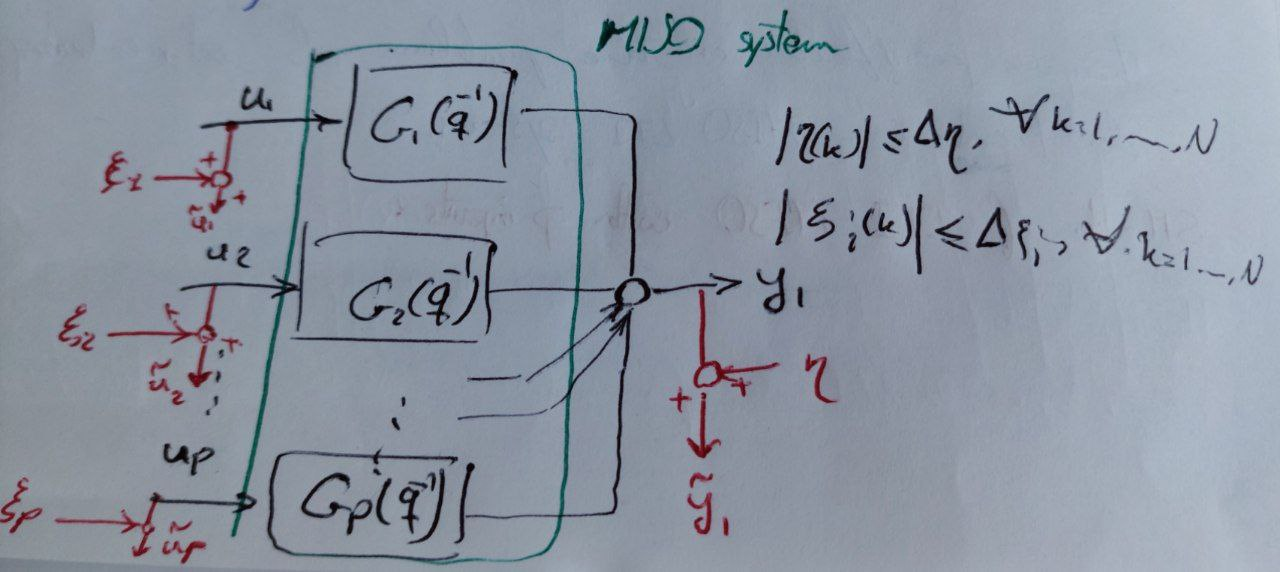
\includegraphics[width=0.85\textwidth]{images/MISO.jpg}
    \caption{The scheme of the error entering the system in an EIV setting.}
    \label{fig:MISO}
\end{figure}

A-posteriori information: N samples of the inputs and the output sequences experimentaly collected. \\
Let's define the feasible parameter set:
\[
\mathcal{D}_\theta= \left\{ \theta \in \mathbb{R}^{\sum_{k=1}^{2n+1}} : 
\begin{array}{l}
y = G_1 u_1 + G_2 u_2 + \cdots + G_p u_p, \\
y = \tilde{y} + \eta, \\
u_1 = \tilde{u}_1 + \xi_1, \, \cdots, \, u_p = \tilde{u}_p + \xi_p, \\
|\xi_1| \leq \Delta \xi_1, \, \cdots, \, |\xi_p| \leq \Delta \xi_p, \, |\eta| \leq \Delta \eta, \, \forall k \in \mathbb{N}
\end{array}
\right\}
\]
So,
\[
\mathcal{D}_\theta = \left\{ \theta \in \mathbb{R}^{\sum_{k=1}^{2n+1}} : 
\begin{array}{l}
y = \frac{\beta_0^1 + \beta_1^1 q^{-1} + \beta_2^1 q^{-2} + \cdots + \beta_n^1 q^{-n}}{1 + \alpha_1^1 q^{-1} + \alpha_2^1 q^{-2} + \cdots + \alpha_n^1 q^{-n}} u_1 + \cdots \\[2ex]+ \frac{\beta_0^p + \beta_1^p q^{-1} + \beta_2^p q^{-2} + \cdots + \beta_n^p q^{-n}}{1 + \alpha_1^p q^{-1} + \alpha_2^p q^{-2} + \cdots + \alpha_n^p q^{-n}} u_p, \\
y = \tilde{y} + \eta, \\
u_1 = \tilde{u}_1 + \xi_1, \, \cdots, \, u_p = \tilde{u}_p + \xi_p, \\
|\xi_1| \leq \Delta \xi_1, \, \cdots, \, |\xi_p| \leq \Delta \xi_p, \, |\eta| \leq \Delta \eta, \, \forall k \in \mathbb{N}
\end{array}
\right\}
\]

How to solve this problem? Mathematically, output is the superposition of the inputs, it might be time consuming, but we can identify single $G_i$'s. In real world problems, nothing is Linear, so different inputs affect the linearity of the system, so MISO problems cannot be written as SISO problems. Now, we should find a solution for our problem.

Consider $G_i(q^{-1}) = \frac{N_i(q^{-1})}{D_i(q^{-1})}$; then, the description of the set becomes as follows:

\[
\mathcal{D}_\theta = \left\{ \theta \in \mathbb{R}^{\sum_{k=1}^{2n+1}} : 
\begin{array}{l}
y = \frac{N_1(D_2.\cdots.D_p)u_1 +N_2(D_1.D_3\cdots.D_p)u_2 + \cdots + N_p(D_1.D_2.\cdots.D_{p-1})u_p}{D_1.D_2\cdots.D_p}\\
y = \tilde{y} + \eta, 
u_1 = \tilde{u}_1 + \xi_1, \, \cdots, \, u_p = \tilde{u}_p + \xi_p, \\
|\xi_1| \leq \Delta \xi_1, \, \cdots, \, |\xi_p| \leq \Delta \xi_p, \, |\eta| \leq \Delta \eta, \, \forall k \in \mathbb{N}
\end{array}
\right\}
\]
\[\Updownarrow\]
\[
\mathcal{D}_\theta= \left\{ \theta \in \mathbb{R}^{\sum_{k=1}^{2n+1}} : 
\begin{array}{l}
(D_1.D_2\cdots.D_p)y = N_1(D_2.\cdots.D_p)u_1 +N_2(D_1.D_3\cdots.D_p)u_2 + \cdots +\\ N_p(D_1.D_2.\cdots.D_{p-1})u_p \:\:
y = \tilde{y} + \eta, 
u_1 = \tilde{u}_1 + \xi_1, \, \cdots, \, u_p = \tilde{u}_p + \xi_p, \\
|\xi_1| \leq \Delta \xi_1, \, \cdots, \, |\xi_p| \leq \Delta \xi_p, \, |\eta| \leq \Delta \eta, \, \forall k \in \mathbb{N}
\end{array}
\right\}
\]
Now, let's focus on the left hand side of the eqation:
\[
(D_1.D_2\cdots.D_p)(\tilde{y}(k)-\eta(k))=\cdots
\]
Let's consider the case where $p = 2$:
\[
(1 + \alpha_1^1 q^{-1} + \alpha_2^1 q^{-2} + \cdots + \alpha_n^1 q^{-n}).(1 + \alpha_1^2 q^{-1} + \alpha_2^2 q^{-2} + \cdots + \alpha_n^2 q^{-n})\cdot(\tilde{y}(k)-\eta(k)) 
\]
Then, the explicit computation will lead to higher order polynomial constraints in the unknown variables, which are $\alpha_1^1\cdots\alpha_n^1$ and $\alpha_1^2\cdots\alpha_n^2$, $\eta(1),\,\eta(2),\, \cdots,\,\eta(k)$.

By following this "standard" approach, we will lead to a polynomial optimization problem, POP, which are of the order $np$. If $p$ is relatively high, we are forced to pick a minimum value of the order of relaxation $\delta$ which is going to be large. We have an explosion of the computational complexity and/or memory overflow, because the size of the data structure involved in the SDP problem obtained by applying the convex relaxation techniques depends explonentially on the order of relaxation. 


\begin{factbox}[Quote]
Always consider that the transient of the system provides information about the poles and the zeros of the system.
\end{factbox}

In order to reduce computational compolexity, let's reformulate the problem by explicitly exploiting the fact that a MISO system is in fact a collection of $p$ SISO system. \\

Let's call, $z_1,\,z_2,\,\cdots,\,z_p$ \textbf{the partial outputs} of the transfer functions $G_1,\,G_2,\,\cdots,\,G_p$:
\[
\begin{array}{c}
z_1 = G_1u_1\\
z_2 = G_2u_2\\
\cdots\\
z_p = G_pu_p
\end{array}
\]

Let's define the FPS: 
\[
\mathcal{D}_\theta = \left\{ \theta \in \mathbb{R}^{\sum_{k=1}^{2n+1}} : 
\begin{array}{l}
\tilde{y} - \eta(k) = z_1(k) + z_2(k) + \cdots + z_p(k) \\
z_1 = G_1u_1,\,
z_2 = G_2u_2,\,
\cdots,\,
z_p = G_pu_p,\,
u_1 = \tilde{u}_1 + \xi_1, \, \cdots, \, u_p = \tilde{u}_p + \xi_p, \\
|\xi_1| \leq \Delta \xi_1, \, \cdots, \, |\xi_p| \leq \Delta \xi_p, \, |\eta| \leq \Delta \eta, \, \forall k \in \mathbb{N}
\end{array}
\right\}
\]

Since $\mathbb{D}_\theta$ depends on $\theta$ but also on many other unknowns, $z_1,\,z_2,\,\cdots,\,z_p$, $\xi_1(1),\,\xi_1(2),\,\cdots,\,\xi_1(N)$ and $\xi_p(1),\cdots,\,\xi_p(N)$, we need to look at the problem in an extended space, which is the space of all the unknown variables.\\
In such a space, we define the Extended Feasible Parameter Set EFPS:


\[
\mathcal{D}_{\begin{array}{l}
\theta,\,z_1,\,z_2,\,\cdots,\,z_p,\,\\\eta,\xi_1,\,\cdots,\,\xi_p
\end{array}
} = \left\{ 
\begin{array}{l}
(\theta,\,\eta,\,\xi_1,\,\cdots,\,z_1,\,z_2,\,\cdots,\,z_p) \in \mathbb{R}^{...} :\\
\tilde{y} - \eta(k) = z_1(k) + z_2(k) + \cdots + z_p(k) \\
z_1(k) = -\alpha_1^1z_1(k-1)-\alpha_2^1z_1(k-2) + \beta_0^1\tilde{u}(k) - \beta_0^1\xi(k) + \cdots \\
+ \beta_{n_1}^1\tilde{u}(k-n_1) - \beta_{n_1}^1\xi_1(k-n_1)\\,
z_2 = \cdots,\,
z_p = \cdots,\,
u_1 = \tilde{u}_1 + \xi_1, \, \cdots, \, u_p = \tilde{u}_p + \xi_p, \\
|\xi_1| \leq \Delta \xi_1, \, \cdots, \, |\xi_p| \leq \Delta \xi_p, \, |\eta| \leq \Delta \eta, \, \forall k \in \mathbb{N}
\end{array}
\right\}
\]

By rewriting the problem exploiting the partial outputs, each sample of the partial outputs, as additional optimization variables, we can rewrite the EFPS in such a way that its mathematical description only involves bilinaer constraints. \textbf{we can again pick as minimum order of relaxation $\delta = 1 $}.
\newpage
\section{Set-membership identification of non-linear systems (discrete-time systems)}

Here, we consider non-linear input-output systems described in regression form:
\[
y(k) = f(\theta,\,r) = f(\theta,\,[y(k-1),\,y(k-2),\,\cdots,\,y(k-n),\,u(k),\,u(k-1),\,u(k-n)])
\]
Where $\theta$ is the vectors of the parameter models and $r$ is the regression.\\
We restrict our attention to the ease where $f$ is a \textbf{multivariate polynomial} funciton of $r(k)$.

\begin{example}[Example 1]
\textbf{A-priori information on the system:}\\
We know from our physical insight that the system is of dynamical order 1 and that $f$ is a multivariate polynomial of order 2.
\[
y(k) = f(\theta,r(k)) = f(\theta,[y(k-1),\,u(k),\,u(k-1))])
\]
In this case, we also have to discuss the degree of the polynomial, in addition to the dynamical order of the system.
\[
y(k) = \theta_1y(k-1) + \theta_2u(k) + \theta_3u(k-1) + \theta_4 y^2(k-1) + \theta_5 u^2(k) +\theta_6 y(k-1)u(k) + \theta_7 y(k-1)u(k-1) + \theta_8 y(k-1)u(k-1) + \theta_9 u(k)u(k-1)
\]
\end{example}

\begin{example}[Example 2]
\textbf{A-priori information on the system:}\\
Dynamical order is 1. and the structure is as follow:
\[
y(k) = \theta_1y(k-1) + \theta_2u(k) + \theta_3u^2(k-1) + \theta_4 y(k-1)u(k)
\]
\end{example}

\begin{example}[Example 3]
\textbf{A-priori information on the system:}\\
We know that the physical system has dynamical order 1 and that in this case we don't have any clear information about the mathematical structure of $f$.
\end{example}

\begin{QandAbox}[Result:]
Assuming that $f$ enjoys some general continuity properties, we can approach the problem by exploiting the so called "stone-weinestress" theorem, which tells us that any non-linear fucntion enjoying continuity property can be approximated as well as we want over a compact set in the regressor space).\\

The stone-weirestress theorem tells us that such a polynomial exists, but the theorem does not provide any information about the structure and the degree of the polynomial.
\end{QandAbox}

 \subsubsection{How to decide the structure and the degree of the polynomial:}
 We starts from polynomial degree 2, and we try to solve the problem:\\
 Is the obtained $\mathbb{D}_\theta$ is empty? This suggests that the POP problem is infeasible; in SparsePOP, this is suggested by \textbf{exit flag -1}.
 \begin{enumerate}
    \item No: Check whether sign($\underline{\theta_i}$) $=$ sign($\overline{\theta_i}$)    \begin{enumerate}
                              \item If the signs are the same. the we are happy :)
                              \item The signs are different:
                                      \begin{itemize}
                                           \item $|\underline{\theta_i}-\overline{\theta_i}|$ is small compared to the noise bound. $\Rightarrow$ $\theta_i = 0$
                                          \item  $|\underline{\theta_i}-\overline{\theta_i}|$ is large and \textbf{the noise bound is big}$\Rightarrow$ \textbf{we have to chage the sensors}!!!
                                          \begin{QandAbox}
                                                The global solution depends on the bound of noise, or how large FPS is. If the noise bound is large, the resultant PUI is large too.
                                          \end{QandAbox}
                                           \item $|\underline{\theta_i}-\overline{\theta_i}|$ is large and \textbf{the sensor bound is small} $\Rightarrow$ \textbf{we have to increase the degree of the polynomial or dynamical order}!!!
                                      \end{itemize}
                              
                         \end{enumerate}
    \item Yes: we can conclude that the selected degree for the polynomial is too low. $\Rightarrow$ \textbf{we have to increase the degree of the polynomial or dynamical order}
 \end{enumerate}
 
 \textbf{Remark}: A similar trial-and-error approachcan also be appllied to the case - both for linear and non-linear system) when the dynamical order is not exactly known from our physical insight.\\
 

\begin{factbox}
Why don't we try to identify gradients of a non-linear system, or our polynomial, which at a certain point is going to be a linear function?

1. We should repeat the identification procedure several times, depending on the degree of the polynomial. (This is not the main issue.)

2. 
\[
\tilde{y} = y + \eta \Rightarrow \frac{d\tilde{y}}{dt} = \frac{dy}{dt} + \frac{d\eta}{dt}
\]


Since the noise is fast-changing, the bound of the derivative of the noise is going to be large.

\textbf{Then, why don't we filter the data?}

1. Because we cannot design a perfect filter.

2. The filter changes the phase of the signal, which in real-time corresponds to a delay. Therefore, by filtering the data, we are no longer identifying the real system.
\end{factbox}

\begin{figure}[htbp]
    \centering
    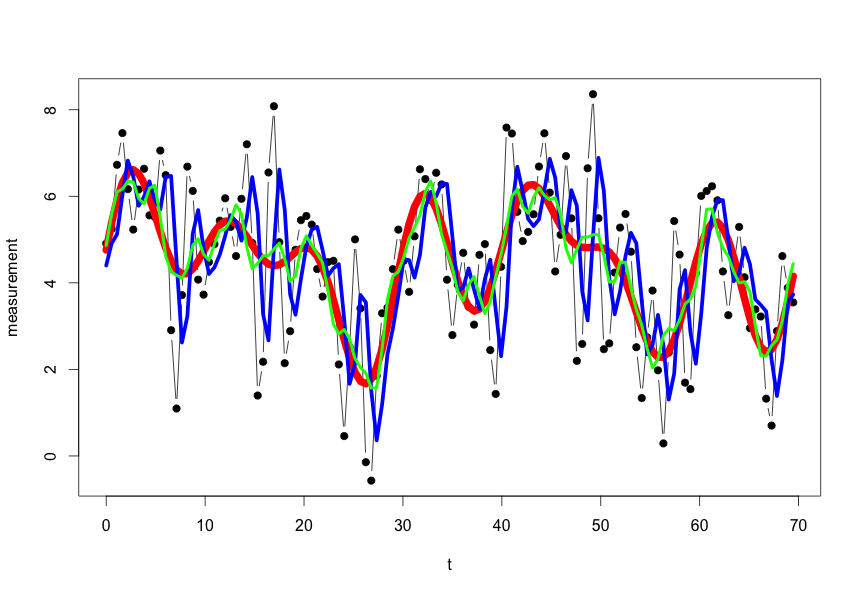
\includegraphics[width=0.7\textwidth]{images/signal-and-noise.png}
    \caption{The scheme of the error entering the system in an EIV setting.}
    \label{fig:signal-and-noise}
\end{figure}

\newpage

\textbf{Question to be pondered on: How to design a filter without the phase shift?}

Now, how to circumvent the explosion of the computational complexity of the convex relaxation approach, when the polynomial involved in the POP have high degrees?\\
Assuming that we want to estimate the parameters of the following non-linear MISO system, which is a \textbf{static system}:
\[
y(k) = \theta_1y(k-1) + \theta_2u_1(k)u_2(k) + \cdots + \theta_n u_1(k)u_2(k)\cdots u_p(k)
\]
where,
\[
\tilde{y}(k) = y(k)+\eta(k) \:\:\forall k
\]
\[
\tilde{u}_i = u(k)+\xi(k)
\]

FPS in this case is defined as follows:
\[
\mathbb{D}_\theta = \{ \theta \in \mathbb{R}^p :\; \tilde{y}(k) - \eta(k) = \theta_1 (\tilde{u}_1(k) - \xi_1(k)) + \cdots + \theta_n \prod_{i=1}^p (\tilde{u}_i(k) - \xi_i(k)),
\]
\[
|\eta(k)| \leq \Delta \eta, \; |\xi_i(k)| \leq \Delta \xi \text{ for all } i \}.
\]

In this case, the problem becomes a POP with constraints of degree$p+1$. Therefore, $\delta \geq \lceil \frac{p+1}{2} \rceil
 $ is going to be large if $p$ is large, possibly being computationally untracktable.\\
 
 In order to reduce the computational complexity of the POP, we can reformulate the problem by intorudcing new variables $z_j$ as follows:
 
 
%this part needs to be corrected
\[
\begin{aligned}
\underline{\theta_1} &= \min\limits_{\theta \in \mathbb{D}_{\eta,\xi,z}} \theta_1 
\text{s.t.} \quad & \begin{aligned}
    z_1 &= \xi_1 \xi_2 \\
    z_2 &= z_1 \xi_3 \\
    z_3 &= z_2 \xi_4 \\
    &\vdots \\
    z_{p-1} &= z_{p-2} \xi_p \\
    \tilde{y}(k) - \eta &= \theta_1 u_1 - \theta_1 \xi_1 + \cdots + \theta_n z_2 z_3 \cdots z_{p-1}
\end{aligned}
\end{aligned}
\]
Here, the structure of the constrains that is defined with slack variables is such that the problem enjoys "the running intersection property", and we can use Sparse relaxation.
Now, we get bilinear constraints, and then, \(\delta_{\text{min}} = 1\).

\section{Set-membership Identification of Block-structured non-linear systems}
Block-structured non-linear systems, or block-oriented non-linear systems, are non-linear dynamical systems which are obtained by connecting together a number of sub-systems such that each one of the subsystems can either be a dynamical LTI system or a static-nonlinear system.
\subsection{Hammerstein Systems}

The block diagram representation of this class of systems is as follows:


\begin{figure}[h!]
\centering
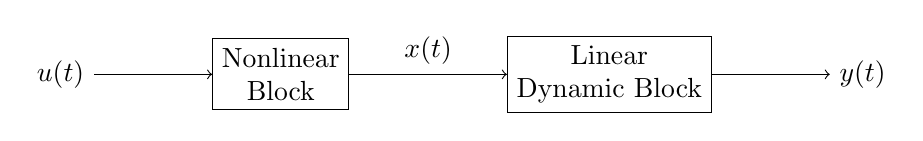
\begin{tikzpicture}[block/.style={rectangle, draw, minimum height=2em, minimum width=3em, align=center}]

    % Define blocks
    \node[block] (nonlinear) {Nonlinear\\Block};
    \node[block, right=2cm of nonlinear] (linear) {Linear\\Dynamic Block};

    % Input and Output
    \node[left=1.5cm of nonlinear] (input) {$u(t)$};
    \node[right=1.5cm of linear] (output) {$y(t)$};

    % Arrows with labels
    \draw[->] (input) -- (nonlinear);
    \draw[->] (nonlinear) -- node[above] {$x(t)$} (linear);
    \draw[->] (linear) -- (output);

\end{tikzpicture}
\caption{Block diagram of a Hammerstein class of non-linear systems}
\label{fig:hammerstein}
\end{figure}

Main features:
\begin{itemize}
    \item The internal signal $x(k)$ cannot be measured
    \item THis structure is useful to describe physical systems which are essentially \textbf{LTI} (as far as the dynamics is concerned), but with a significant input non-linearity, e.g. presence of input saturation or deadzone non-linearity or any other non-linearity effect in the actuation part due to friction or other physical reasons.
\end{itemize}

Mathematical description of Hammerstein systems is as follows:
\[
\begin{cases}
\text{LTI block:}\\G(q^{-1}) = -\alpha_1y(k-1) - \alpha_2y(k-2) -\cdots -\alpha_ny(k-n)+\beta_0x(k)+\beta_1x(k-1)+\cdots + \beta_nx(k-n)\\
\text{Non-linear block:} \\x(k) = \mathcal{N}(u(k))
\end{cases}
\]

Additional assumption about the state of $N(.)$:
\[
x(k) = N(u(k)) = \sum_{j = 1}^{m}\gamma_j\phi_j(u(k))) = \gamma_1\phi_1(u(k)) + \gamma_2\phi_2(u(k)) + \cdots + \gamma_m\phi_m(u(k))
\]

where, $\{\phi_j\},\,j = 1,\,2,\,\cdots,\,m$ is a set of \textbf{basis function} selected based on our physical insight.

In the case we don0t have any specific physical insight on the form of $\mathcal{N}$, we can surely select $\{\phi_j\}$ to be the standard polynomial basis function.

\[
\begin{cases}
\phi_1(u(k)) = u(k)\\
\phi_2(u(k)) = u^2(k)\\
\cdots\\
\phi_m(u(k)) = u^m(k)
\end{cases}
\]
Pay attention that no offset is considered for $x$, bacause when the input is switched off, it is non-sence to have output.\\

\subsubsection{Output-Error setting for the Hammerstein system structure}
A-priori information about the system structure:
\begin{itemize}
    \item The system has a Hammerstein structure.
    \item $x$ is a linear combination of basis functions
    \item $x$ cannot be measured
    \item $y$ is an LTI system with the input $x$.\\
    \[
    y(k) = -\alpha_1y(k-1) - \alpha_2y(k-2) - \cdots - \alpha_n y(k-n) + \beta_0 x(k) + \beta_1 x(k-1) + \cdots + \beta_n x(k-n)
    \]
\end{itemize}

A-priori information about noise structure:
\begin{itemize}
    \item We consider an output-error, for now.
    \item Each sample of the noise is bounded by $\Delta \eta$
\end{itemize}

A-posteriori information: the input-output data samples.

\subsubsection{Feasible Parameter Set $\mathbb{D}_\theta$}
\[
\begin{array}{l}
\mathbb{D}_\theta = \{\theta \in \mathbb{R}^{2n + 1 + m}: 
    y(k) = -\alpha_1y(k-1) - \alpha_2y(k-2) - \cdots - \alpha_n y(k-n) + \beta_0 x(k) + \beta_1 x(k-1) + \cdots \\+ \beta_n x(k-n), x(k) = \gamma_1\phi_1(u(k)) + \gamma_2\phi_2(u(k)) + \cdots + \gamma_m\phi_m(u(k))
\tilde{y}(k) = y + \eta(k),\,|\eta(k)|\leq \Delta\eta
\}
\end{array}
\]
First approach:

\[
\begin{array}{l}
\mathbb{D}_\theta = \{\theta \in \mathbb{R}^{2n + 1 + m}: 
    \tilde{y}(k)-\eta(k) = -\alpha_1[\tilde{y}(k-1)-\eta(k-1)] - \cdots - \alpha_n [\tilde{y}(k-n)-\eta(k-n] +\\ \beta_0 [\gamma_1 u(k) + \gamma_2 u^2(k) + \cdots+ \gamma_m\phi_m(u(k))] +\cdots
    + \beta_n [\gamma_1 u(k-n) + \gamma_2 u^2(k-n) + \cdots+ \gamma_m\phi_m(u(k-n))]\\,\,|\eta(k)|\leq \Delta\eta
\}
\end{array}
\]

Regarding the same reasoning that have been done before, we need to move from FPS to EFPS so that we include a larger space including the noise samples as its variables.
\[
\mathbb{D}_{\theta,\,\eta}
\]

\subsubsection{EIV setting for the Hammerstein system structure}

Here, we consider that the exact value of the inputs are not known, and input samples are corrupted with the noise as well.\\
In this case, if we consider $\{\phi_j\}$ other than polynomial basis, the dependancy of $\{\phi_j\}$ with respect to the error $\xi(k)$ is no more polynomial, \textbf{thereby we are not going to obtain POPs in order to compute PUIs.} As a consequence, we don't know how to approximate the global optimal solution of the optimization problem to be solved to compute the PUI. 

\begin{factbox}
For Hammerstein system structure, whenever the input measurements are corrupted by noise, we have to select the set of basis functions to be a set of polynomial function.
\end{factbox}

Considering a set of polynomial basis funcitons, the dependancy of $x$ and $\xi$ becomes polynomial, but the polynomials that are obtained are of a significantly large degrees in general.\\
PUI's can be computed by selecting POPs, but $\delta$, or relaxation order, is going to be large. Therefore, we are in trouble from the computational point of view. The idea is to avoid replacing $x(k)$ inside the description of the LTI subsystem. We directly move to the following description of the EFPS.
\[
\begin{array}{l}
\mathbb{D}_{\theta,\eta,\xi} = \{\theta \in \mathbb{R}^{2n + 1 + m},\,\eta \in \mathbb{R}^N,\,\xi \in \mathbb{R}^N: 
    y(k) = -\alpha_1y(k-1) - \alpha_2y(k-2) - \cdots - \alpha_n y(k-n) + \\ \beta_0 x(k) + \beta_1 x(k-1) + \cdots + \beta_n x(k-n), x(k) = \gamma_1\phi_1(u(k)) + \gamma_2\phi_2(u(k)) + \cdots + \gamma_m\phi_m(u(k))\\
\tilde{y}(k) = y + \eta(k),\,|\eta(k)|\leq \Delta\eta
\}
\end{array}
\]

In this second approach, we have again a set of described by bilinear constraints involving as optimization variable of the samples and also the unmeasureable inner signal $x(k)$.

\[
PUI_{\theta_i} = [\underline{\theta_i},\,\overline{\theta_i}]
\]

\[
\begin{cases}
\underline{\theta_i} = \min \limits_{\theta_i \in \mathbb{\mathbb{D}_{\theta,\,\xi,\,\eta}}} \theta_i\\
\underline{\theta_i} = \min \limits_{\theta_i \in \mathbb{\mathbb{D}_{\theta,\,\xi,\,\eta}}} -\theta_i\\
\end{cases}
\]
\begin{QandAbox}
Polynomials cannot be used to model saturation, globally, but for a bounded range they can. 
\end{QandAbox}

\subsubsection{Identifiability of Hammerstei systems:}
Let's consider the following two hammerstein system.
\[
\begin{cases}
y1 = G_1(q^{-1})\mathcal{N}_1(u(k))\\
y2 = G_2(q^{-1})\mathcal{N}_2(u(k))
\end{cases}
\]
It can be easily proved that, $y_1 \equiv y_2\,\,\,\forall u$ provided that $\mathcal{N}_1 = \alpha \mathcal{N}_2$, $G_2(q^{-1}) = \alpha G_1(q^{-1}) \:\:\:\forall \alpha \in \mathbb{R}$.\\

The Hammerstein system is not \textbf{itentifiable} because we have an infinit number of solutions to the identification problem, which are perfectly equivalent from the input-output point of view.\\

\subsubsection{Results}
\begin{itemize}
    \item No matter what is the technique that we are going to use, we will not be able to estimate the exact parameter of the true Hammerstein system, even if we collect noiseless data and $N \to \infty$
    \item since we have an infinite number of Hamerstein model able to provide exactly the same input-output behavior of the true one, our numberical procedure for the computation of the PUIs is going to fail. WHY???  \textbf{Because the FPS set is going to be structurally unbounded} For each value of $\alpha$ a feasible unceratinty set is going to be obtained, and when they are put next to one another, the result is going to be an unbounded FPS.
\end{itemize}

Therefore, we need to add additional constraints to make it bounded.

\begin{figure}[htbp]
    \centering
    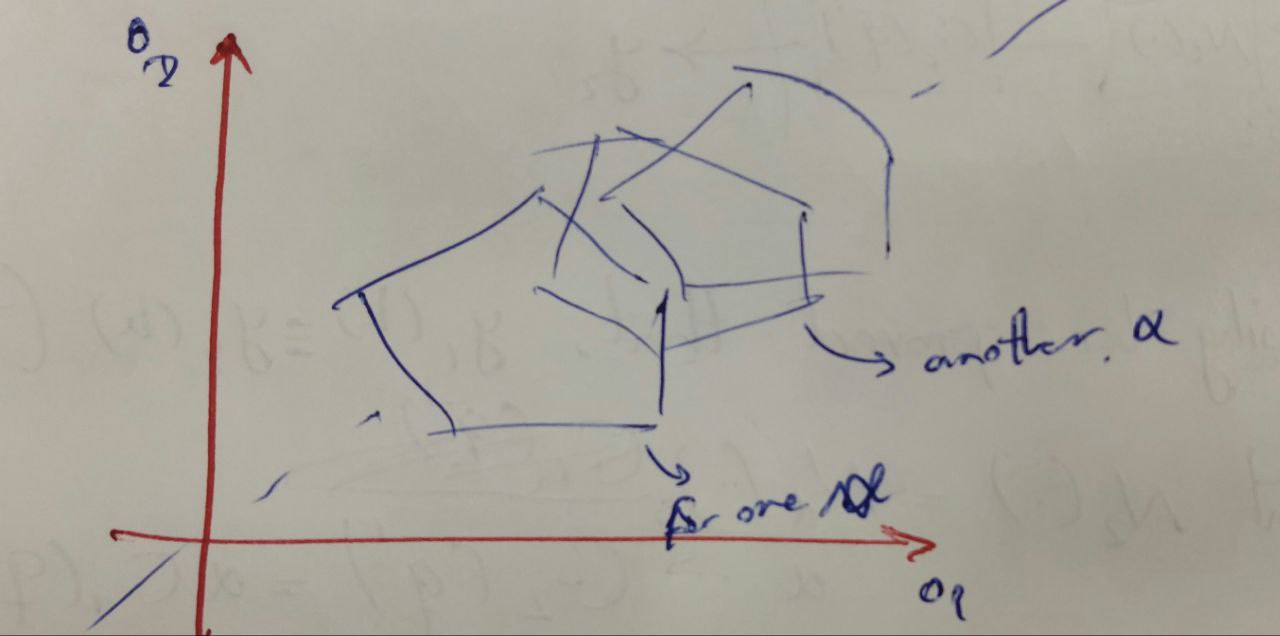
\includegraphics[width=0.5\textwidth]{images/unidentifiability_hammer.jpg}
    \caption{A representation of the unidentifiability issue of Hammerstein nonlinear systems.}
    \label{fig:signal-and-noise}
\end{figure}

Having said so, before attempting to solve the problem, identifiability of the system should be checked.

\subsubsection{How to force uniquness of the solution in the Set-membership identification of Hammerstein systems?}
\begin{enumerate}
    \item Due to discussion we had in the previous lesson. We have to conclude that it's not possible to identify the true Hammerstein system under study even if the collected data are noiseless.
    \item However, if we want to model the system under study in order to: 
    \begin{itemize}
        \item design a controller
        \item predict the ouput behavior 
    \end{itemize}
    then, eahc one of Hammerstein system that provide same input-output behavior are perfectly fine.
    \item Then, in order to force uniqueness of solution, we  have to add to the description of FPS and of the EFPS one more additional constraints such that, thanks to that condition, we force identifiability without changing the global input-output behavior mapping.
\end{enumerate}

\textbf{Possible additional constains to force uniquness are:}\\
\begin{itemize}
    \item dcgain('LTI part of the system')=1
    \item setting one of the parameters of the non-linear part of the system to 1, e.g.$\gamma_1 = 1$
\end{itemize}
Now, it should be checked if the additional constraint is a polynomial constraint. For the second item abovementioned, it is trivial. It can easily be shown that also the first type of constraints are polynomial, or at any rate linear. For a second-order system, it is as follows:
\[
G(z) = \frac{\theta_3z + \theta_4}{z^2 + \theta_1z + \theta_1}
\]
Since we assume that our systems are BIBO stable, we know that we don't have any pole at 1. In the discrete-time case.
\[
\text{dcgain}(G(z)) = 1 \Rightarrow \theta_3 + \theta_4 - \theta_2 - \theta_1 = 0
\]

\textbf{Important remark:} The correct formulation of FPS or EFPS for the Hammerstein system must include either of the two additional constraints to lead to a unique solution.


\subsection{Wiener System}
Another basic structure in the class of block-structured nonlinear systems.





\begin{figure}[h!]
\centering
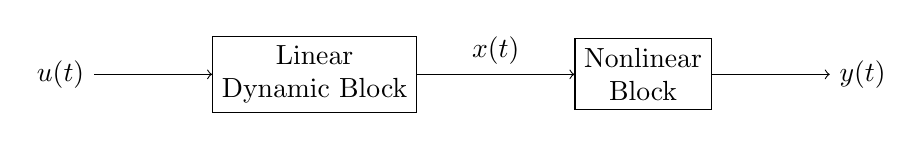
\begin{tikzpicture}[block/.style={rectangle, draw, minimum height=2em, minimum width=3em, align=center}]

    % Define blocks
    \node[block] (linear) {Linear\\Dynamic Block};
    \node[block, right=2cm of linear] (nonlinear) {Nonlinear\\Block};

    % Input and Output
    \node[left=1.5cm of linear] (input) {$u(t)$};
    \node[right=1.5cm of nonlinear] (output) {$y(t)$};

    % Arrows with labels
    \draw[->] (input) -- (linear);
    \draw[->] (linear) -- node[above] {$x(t)$} (nonlinear);
    \draw[->] (nonlinear) -- (output);

\end{tikzpicture}
\caption{Block diagram of a Hammerstein class of non-linear systems}
\label{fig:hammerstein}
\end{figure}


The same of the previous system, $N(.)$ is the output of a non-linear static map.

Useful to describe non-linear dynamical systems wherer the dynamics is LTI, but we can have a significant non-linear output distortion due, for example, to some non-linear effect in the sensor.\\
The set-membership identification of Weiner system is quite similar to that of Hammerstein sysetm - including the discussion that we had about identifiability and uniquness of the solution.

ELABORATION OF THESE KIND OF SYSTEMS IS LEFT AS AN EXERCISE TO THE STUDENTS.
\subsection{Lur'e System}
In this class of non-linear system, the system has a closed-loop internal structure where the feedforward path is an LTI system and the nonlinearity is a static transfer function on the feedbakc of the system.

\begin{figure}[htbp]
    \centering
    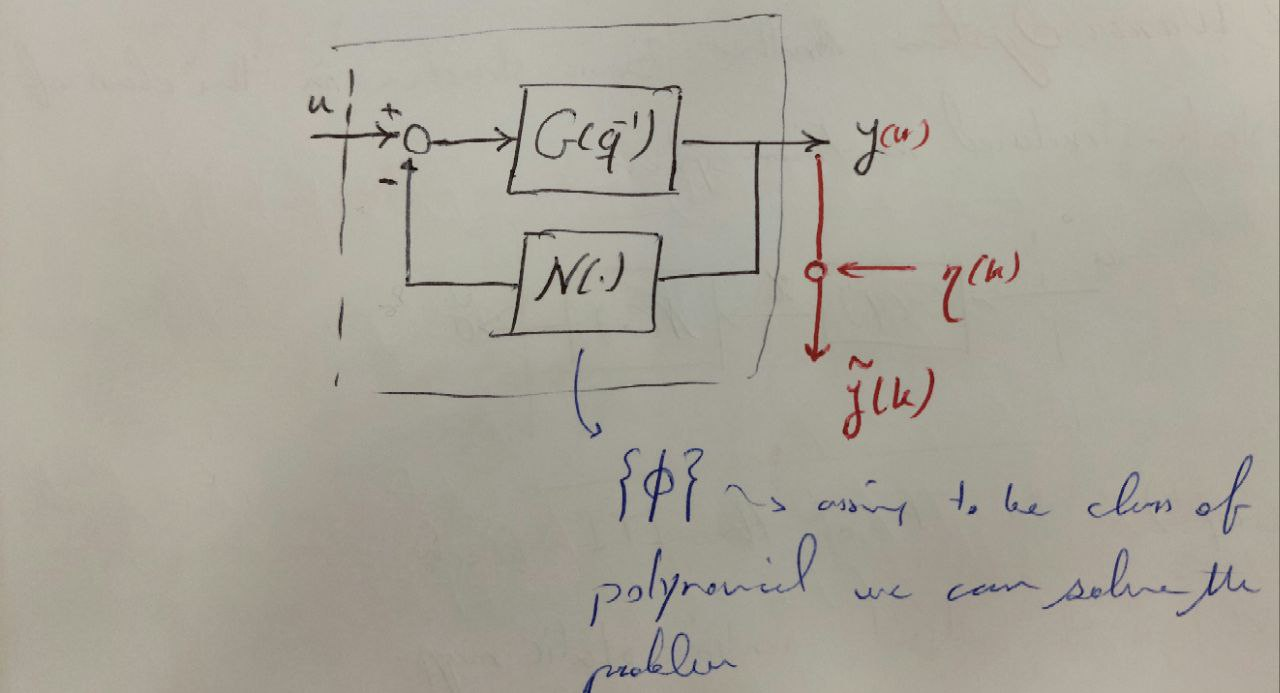
\includegraphics[width=0.75\textwidth]{images/Lure.jpg}
    \caption{A block diagram representation of Lur'e class of the system.}
    \label{fig:signal-and-noise}
\end{figure}

In this case, again, it is required to add another constraint in order to guarantee the uniqueness of the solution. In this case, however, it is a bit tricky to do so.

ELABORATION OF THESE KIND OF SYSTEMS IS LEFT AS AN EXERCISE TO THE STUDENTS.

\subsection{Generalization of block-structured models:}

\begin{figure}[H]
    \centering
    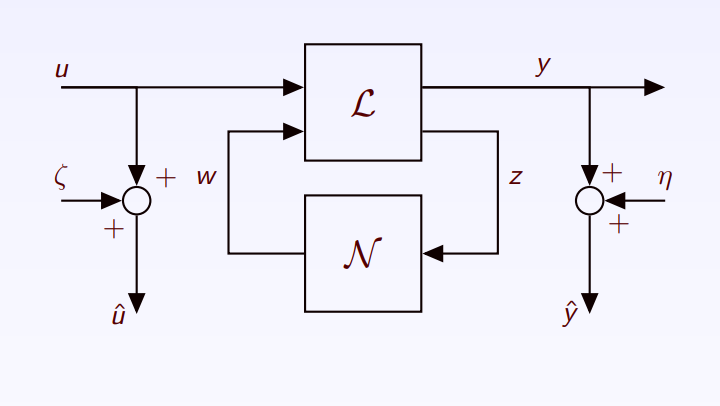
\includegraphics[width=0.75\textwidth]{GBSC.png}
    \caption{Block diagram representation of generalized block-structured configuration}
\end{figure}

$\mathcal{L}$ is a multivariable linear dynamic system described by a MIMO transfer matrix, mapping the noiseless inputs $\mathbf{u}_t \in \mathbb{R}^{n_u}$ and $\mathbf{w}_t \in \mathbb{R}^{n_w}$ into the noiseless outputs $\mathbf{z}_t \in \mathbb{R}^{n_z}$ and $\mathbf{y}_t \in \mathbb{R}^{n_y}$; Here, $w$ and $z$ are called internal inputs and internal outputs, respectively.
    \[
    \begin{bmatrix}
    \mathbf{y}_t \\
    \mathbf{z}_t
    \end{bmatrix}
    = \mathcal{L}
    \begin{bmatrix}
    \mathbf{u}_t \\
    \mathbf{w}_t
    \end{bmatrix}
    =
    \begin{bmatrix}
    \mathcal{L}_{yu} & \mathcal{L}_{yw} \\
    \mathcal{L}_{zu} & \mathcal{L}_{zw}
    \end{bmatrix}
    \begin{bmatrix}
    \mathbf{u}_t \\
    \mathbf{w}_t
    \end{bmatrix}
    \]
The generic $(i,j)$-th entry of the matrix $\mathcal{L}$ is a SISO transfer function:
    \[
    \mathcal{L}(i,j) = G^{(i,j)}(q^{-1}) = \frac{\sum_{m=0}^{n_b^{(i,j)}} b_m^{(i,j)} q^{-m}}{1 + \sum_{k=1}^{n_a^{(i,j)}} a_k^{(i,j)} q^{-k}}
    \]
$q^{-1}$ is the backward time shift operator.

The nonlinear block $\mathcal{N}$ is an array of nonlinear static functions:
    \[
w_t^{(i)} = f^{(i)}(\mathbf{z}_t), \quad i = 1, \dots, n_w
    \]
$f^{(i)}(\mathbf{z}_t)$ is defined as:
    \[
    f^{(i)}(\mathbf{z}_t) = \sum_{k=1}^{n_\phi^{(i)}} \phi_k^{(i)} \Phi_k^{(i)}(\mathbf{z}_t)
    \]
$\Phi_k^{(i)}: \mathbb{R}^{n_z} \to \mathbb{R}$ are known nonlinear multivariate polynomial basis functions.


\subsection{Noise Structures (EIV Set-Up)}

Input and output signals are affected by additive noise:
    \[
    \tilde{u}_t^ = u_t + \zeta_t, \quad \tilde{y}_t = y_t + \eta_t
    \]
  The noise signals are unknown but bounded:
    \[
    |\boldsymbol{\zeta}_t| \leq \Delta_{\zeta}, \quad |\boldsymbol{\eta}_t| \leq \Delta_{\eta} \quad \forall t
    \]

\subsection{Parameter Vector}

The system parameter vector is defined as:
\[
\boldsymbol{\theta} = [\boldsymbol{\theta}_L, \boldsymbol{\theta}_N]^T \in \mathbb{R}^p
\]

 $\boldsymbol{\theta}_L \in \mathbb{R}^{p_l}$ and $\boldsymbol{\theta}_N \in \mathbb{R}^{p_n}$ correspond to the parameters of the linear and nonlinear subsystems respectively, where $p = p_l + p_n$.


\subsection{Identifiability}

The model equations for identifiability are given as:

\[
\begin{bmatrix}
\mathbf{y}_t \\
\mathbf{z}'_t
\end{bmatrix}
=
\begin{bmatrix}
\mathcal{L}_{yu} & \mathcal{L}_{yw}\mathbf{K}_w^{-1} \\
\mathbf{K}_z\mathcal{L}_{zu} & \mathbf{K}_z\mathcal{L}_{zw}\mathbf{K}_w^{-1}
\end{bmatrix}
\begin{bmatrix}
\mathbf{u}_t \\
\mathbf{w}'_t
\end{bmatrix}
=
\mathcal{L}'
\begin{bmatrix}
\mathbf{u}_t \\
\mathbf{w}'_t
\end{bmatrix}
\]

The nonlinear block is redefined as:
\[
\mathbf{w}'_t = \mathcal{N}'(\mathbf{z}'_t) = \mathbf{K}_w\mathbf{\Gamma}(\mathbf{z}'_t)
\]

\begin{itemize}
    \item $\mathbf{K}_w$ and $\mathbf{K}_z$ are invertible constant matrices of suitable dimensions.
    \item $\mathbf{\Gamma}$ is a stack of nonlinear polynomial static functions:
    \[
    g^{(i)}(\mathbf{z}_t) = \sum_{k=1}^{n_\phi^{(i)}} \psi_k^{(i)} \Phi_k^{(i)}(\mathbf{z}'_t)
    \]
    \item The coefficients $\psi_k^{(i)}$ satisfy:
    \[
    \mathbf{\Gamma}(\mathbf{z}'_t) = \mathcal{N}(\mathbf{z}_t)
    \]
\end{itemize}

\subsection{Identifiability}

The general block-structured nonlinear system is not identifiable since systems $(\mathcal{N}, \mathcal{L})$ and $(\mathcal{N}', \mathcal{L}')$ exhibit the same mapping between $\mathbf{u}$ and $\mathbf{y}$. To impose identifiability:

\[
\sum_{m=0}^{n_b^{(i,j)}} b_m^{(i,j)} = 1 + \sum_{k=1}^{n_a^{(i,j)}} a_k^{(i,j)}
\]

The steady-state gains of all transfer functions in submatrices $\mathcal{L}_{yw}$ and $\mathcal{L}_{zu}$ are set to one.

\subsection{Extended Feasible Parameter Set (EFPS)}

The Extended Feasible Parameter Set (EFPS) $\mathcal{D}$ is defined as follows:

\[
\mathcal{D} = \left\{
(\boldsymbol{\theta}, \mathbf{v}^{(i,j)}, \boldsymbol{\eta}, \mathbf{w}, \mathbf{z}) \in \mathbb{R}^p + (\mathbb{R}^r + \mathbb{R}^s)^N :
\right.
\]
\[
\mathbf{v}_t^{(i,j)} = \sum_{m=0}^{n_b^{(i,j)}} b_m^{(i,j)} \mathbf{r}_{t-m}^{(j)} - \sum_{k=1}^{n_a^{(i,j)}} a_k^{(i,j)} \mathbf{v}_{t-k}^{(i,j)},
\]
\[
\mathbf{s}_t^{(i)} = \sum_{k=1}^{n_r} \mathbf{v}_t^{(i,k)}, \quad \forall i = 1, \dots, n_s,
\]
\[
\mathbf{w}_t^{(l)} = \sum_{k=1}^{n_\phi^{(l)}} \phi_k^{(l)} \Phi_k^{(l)}(\mathbf{z}_t),
\]
\[
\mathbf{y}_t^\ast = \mathbf{y}_t + \boldsymbol{\eta}_t, \quad \|\boldsymbol{\eta}\| \leq \Delta_\eta,
\]
\[
\mathbf{u}_t^\ast = \mathbf{u}_t + \boldsymbol{\zeta}_t, \quad \|\boldsymbol{\zeta}\| \leq \Delta_\zeta,
\]
\[
t = 1, \dots, N, \quad i = 1, \dots, n_s, \quad j = 1, \dots, n_r,
\]
\[
l = 1, \dots, n_w, \quad o = 1, \dots, n_y, \quad i = 1, \dots, n_u
\}
\]

Here:

\begin{itemize}
    \item $\mathbf{v}_t^{(i,j)}$ represents the partial outputs, defined explicitly as:
    \[
    \mathbf{v}_t^{(i,j)} = G^{(i,j)}(q^{-1}) \mathbf{r}_t^{(j)} = \sum_{m=0}^{n_b^{(i,j)}} b_m^{(i,j)} \mathbf{r}_{t-m}^{(j)} - \sum_{k=1}^{n_a^{(i,j)}} a_k^{(i,j)} \mathbf{v}_{t-k}^{(i,j)}.
    \]
    \item $\mathbf{r}_t = [\mathbf{u}_t, \mathbf{w}_t]^T \in \mathbb{R}^{n_r}$ is a vector of system inputs.
    \item $\mathbf{s}_t = [\mathbf{y}_t, \mathbf{z}_t]^T \in \mathbb{R}^{n_s}$ is a vector of system states.
    \item The term $\mathbf{w}_t^{(l)}$ involves the nonlinear polynomial functions $\Phi_k^{(l)}$.
\end{itemize}
The EFPS represents the set of all possible system configurations that satisfy the constraints imposed by the model equations, noise bounds, and system parameters.


\subsection{Parameter Uncertainty Intervals (PUI)}

The EFPS $\mathcal{D}$ allows for computation of the parameter uncertainty intervals:
\[
\text{PUI}_k = [\theta_k^\text{min}, \theta_k^\text{max}]
\]

These are determined by solving global optimization problems:
\[
\theta_k^\text{min} = \min_{\boldsymbol{\theta} \in \mathcal{D}} \theta_k, \quad \theta_k^\text{max} = \max_{\boldsymbol{\theta} \in \mathcal{D}} \theta_k
\]

\subsection{Bounds Computation as Polynomial Optimization}

The bounds are computed by solving the following optimization problem:
\[
\begin{aligned}
    \min_{\boldsymbol{\theta}, \mathbf{v}^{(i,j)}, \boldsymbol{\eta}, \mathbf{w}, \mathbf{z}} \quad & \theta_k \quad \text{(or maximize $\theta_k$ for upper bound)} \\
    \text{s.t.} \quad & \mathbf{v}_t^{(i,j)} = \sum_{m=0}^{n_b^{(i,j)}} b_m^{(i,j)} \mathbf{r}_{t-m}^{(j)} - \sum_{k=1}^{n_a^{(i,j)}} a_k^{(i,j)} \mathbf{v}_{t-k}^{(i,j)}, \\
    & \mathbf{s}_t^{(i)} = \sum_{k=1}^{n_r} \mathbf{v}_t^{(i,k)}, \quad \forall i = 1, \dots, n_s, \\
    & \mathbf{w}_t^{(l)} = \sum_{k=1}^{n_\phi^{(l)}} \phi_k^{(l)} \Phi_k^{(l)}(\mathbf{z}_t), \quad \forall l = 1, \dots, n_w, \\
    & \mathbf{y}_t^\ast = \mathbf{y}_t + \boldsymbol{\eta}_t, \quad \|\boldsymbol{\eta}\| \leq \Delta_\eta, \\
    & \mathbf{u}_t^\ast = \mathbf{u}_t + \boldsymbol{\zeta}_t, \quad \|\boldsymbol{\zeta}\| \leq \Delta_\zeta, \\
    & t = 1, \dots, N, \quad i = 1, \dots, n_s, \quad j = 1, \dots, n_r, \\
    & l = 1, \dots, n_w, \quad o = 1, \dots, n_y, \quad i = 1, \dots, n_u.
\end{aligned}
\]


\section*{Final Remarks}

\begin{itemize}
    \item Global optimal solutions can be computed using Lasserre-relaxation methods.
    \item Specific cases like Hammerstein, Wiener, and Lur’e systems are included within the GBSC framework.
    \item SISO and MIMO LTI systems are also special cases.
    \item General polynomial nonlinear systems in regressor form can be analyzed under this framework.
\end{itemize}

\section*{Further Reading}

\begin{itemize}
    \item V. Cerone et al., *A unified framework for the identification of a general class of multivariable nonlinear block-structured systems*, International Journal of Robust and Nonlinear Control, 2021.
    \item V. Cerone et al., *One-shot set-membership identification of generalized Hammerstein-Wiener systems*, Automatica, 2020.
    \item V. Cerone et al., *Bounding the parameters of block-structured nonlinear feedback systems*, International Journal of Robust and Nonlinear Control, 2013.
\end{itemize}
\chapter{Continuous-Time Identification}

We start this discussion considering LTI SISO models.\\

The problem involves finding the parameters \(\theta\) of a model of the form:
\[
H(s, \theta) = \frac{\beta_{n-1}s^{n-1} + \beta_{n-2}s^{n-2} + \cdots + \beta_1s + \beta_0}{s^n + \alpha_{n-1}s^{n-1} + \alpha_{n-2}s^{n-2} + \cdots + \alpha_1s + \alpha_0}
\]
where
\[
\theta = [\alpha_1, \alpha_2, \ldots, \alpha_{n-1}, \beta_0, \ldots, \beta_{n-1}]
\]

This problem needs to be solved using noisy and sampled data. The block diagram scheme for this problem is shown below:

\begin{figure}[htbp]
    \centering
    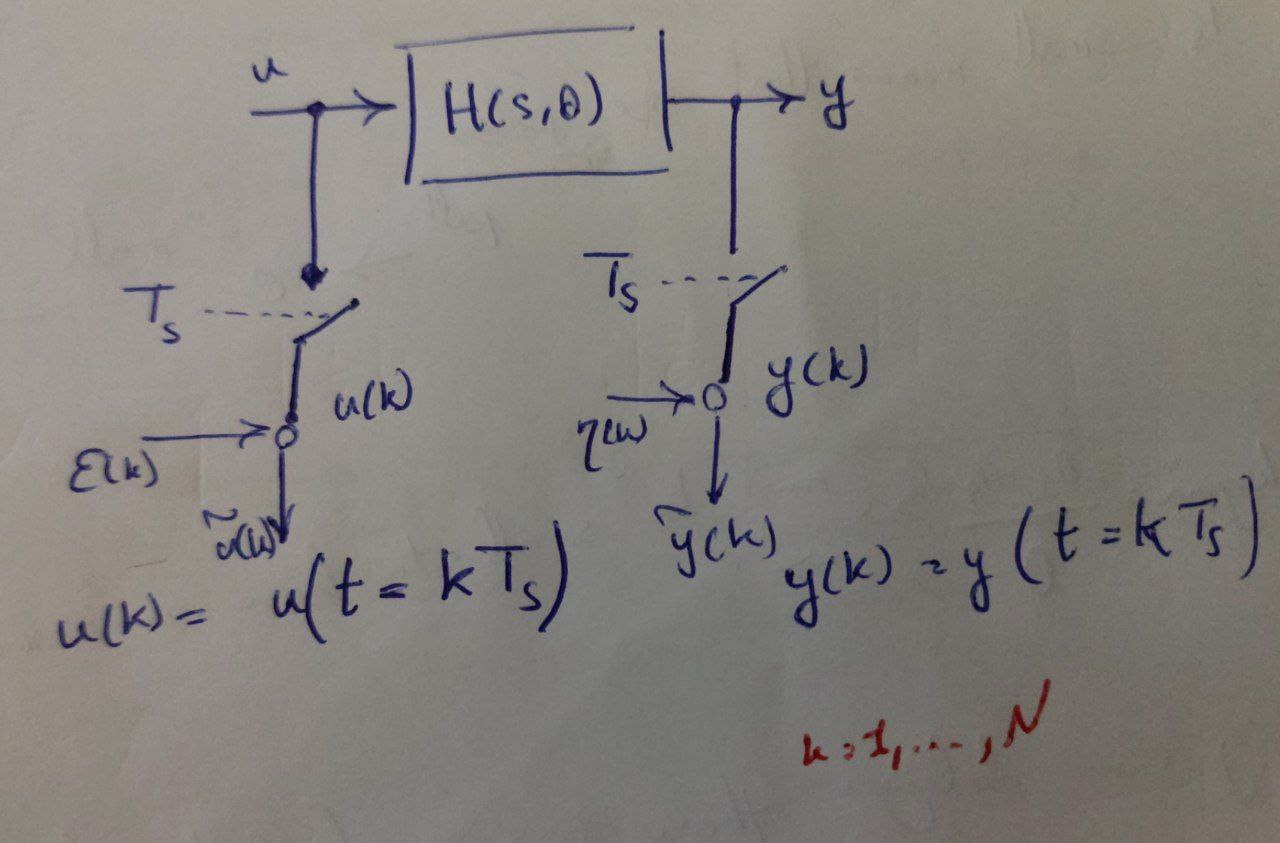
\includegraphics[width=0.7\textwidth]{images/continuous-scheme.jpg}
    \caption{Block diagram representation of sampling data in the continuous scheme.}
    \label{fig:signal-and-noise}
\end{figure}

\textbf{Motivations:}
\begin{enumerate}
    \item By nature, the parameter vector \(\theta\) does not depend on the sampling rate \(T_s\).\\
    When \(T_s\) decreases, all the poles tend to 1. In particular, the poles of a DT system obtained by discretization of a continuous-time system are:
    \[
    P_{dt} = e^{-P_{ct}T_s}
    \]
    Consequently, to maintain a bounded DC gain, the parameters of the numerator tend to zero.

    \item Continuous-time models are closer to the physical description of systems.

    \item Most robust control design techniques are formulated in continuous-time, e.g., \(H_\infty\) and \(\mu\)-synthesis.
\end{enumerate}

\textbf{Two Families of Approaches for System Identification in This Domain:}
\begin{enumerate}
    \item \textbf{Indirect approach:}\\
    
    \begin{itemize}
        \item Estimate a discrete-time model from data.
        \item Use an inverse discretization method to transform this model into continuous-time:
        \[
        u(k) \xrightarrow{\text{Standard discrete identification}} H(q^{-1}, \theta) \xrightarrow{\text{Inverse discretization}} H(s, \theta_c)
        \]
    \end{itemize}
    This approach is simple but has some issues:
    \begin{itemize}
        \item It is not true continuous-time identification. This approach does not solve issues related to the choice of the sampling rate.
        \item Inverse discretization methods, in general, do not preserve important system properties such as stability.
    \end{itemize}

\begin{example}[MATLAB Code]
\begin{verbatim}
theta_LS = A\B; % LS estimation for the DT model
H_z = tf(theta_LS, theta_LS, T_s); % DT model transfer function
H_s = d2c(H_z, 'method'); % Convert to CT model
\end{verbatim}

For the method, you can use \texttt{'zoh'}. Note that the continuous-time parameters will be correct if the following conditions hold:

\begin{enumerate}
    \item The discrete-time parameters are accurate.
    \item \(u(t)\) remains constant over each time interval \([k, k+T_s]\), meaning the sampling rate is much faster than the dynamics of the actuator, look at the following figure.
\end{enumerate}

Another method is \textit{matched} which does the following:
\[
p^{ct} = \frac{\ln(p^{dt})}{T_s}
\]
\end{example}

\begin{figure}
    \centering
    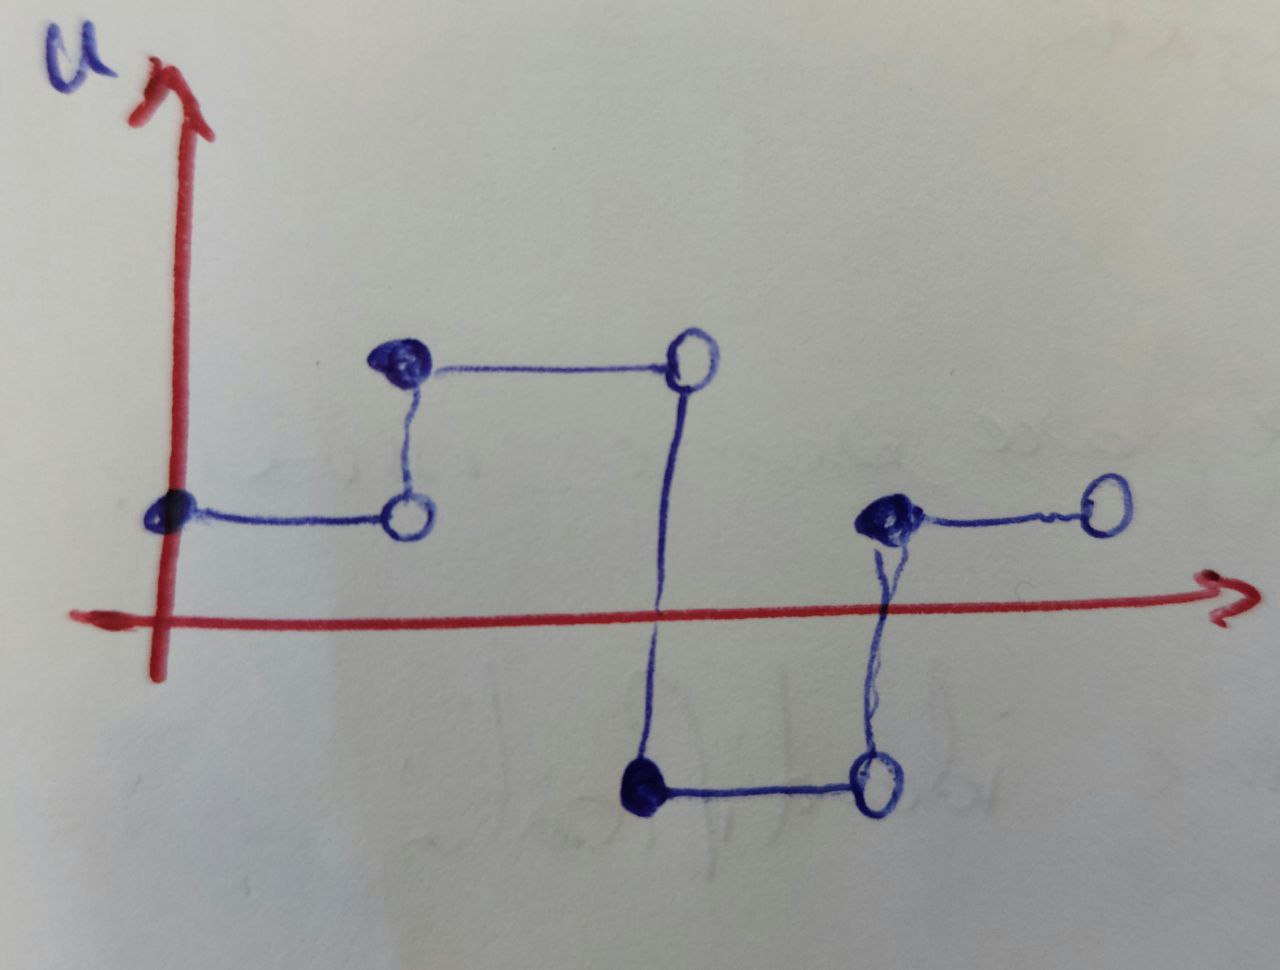
\includegraphics[width=0.35\textwidth]{images/discretized-input.jpg}
    \caption{A discretized input; notice that the value of \( u \) remains constant between consecutive sampling instances.}
\end{figure}
\newpage
    \item \textbf{Direct approach}\\
    
Let us consider a simple example:
\[
H(s) = \frac{\beta_0 + \beta_1s}{s + \alpha_0}
\]
\[
y(s) = H(s) u(s)
\]
Considering zero initial condition for our system:
\[
s y(s) + \alpha_0 y(s) = \beta_1 s u(s) + \beta_0 u(s)
\]
\[
\xrightarrow{\mathcal{L}^{-1}} \dot{y}(t) + \alpha_0 y(t) = \beta_1 \dot{u}(t) + \beta_0 u(t)
\]
Notice that if we could measure $\dot{y}(t)$ and $\dot{u}(t)$, by taking sampled measurements. We could use LS in order to solve the problem, by shaping the regression matrix and output matrix.


\subsubsection{How to obtain $\dot{y}(k)$ and $\dot{u}(t)$ }
We cannot use a derivative block, since it is anti-causal, the best case is implementing a high-pass filter, but we know that a high-pass filter amplifies the noise.\\

We try to estimate them:
\[
\dot{y}(t) = D(q^{-1})y(k)
\]
where $D$ is some discretization of $H(s) = s$.\\

This is a numerical derivative method. The problem is that we need to do this using measured output samples. Therefore, if the measurements have high-freuqnecy components, or at any rate noise, they would be amplified.
\[
\dot{y}(k) = D(q^{-1})y(k) +D(q^{-1})\eta(k)
\]

Another important aspect to take into consideration is that, in this method, the noises becomes correlated, even if the original noise samples are not correlated, and for this reason we cannot employ Least Squared method.\\

\textbf{Instead we try to estimate the following signals:}
\[
y^{I}(t) = \mathcal{L}^{-1}\{Y^{I}(s)\} \:\:\text{ where }\:\: Y^{I}(s) = \lambda(s) Y(s)
\]
\[
u^{I}(t) = \mathcal{L}^{-1}\{U^{I}(s)\} \:\:\text{ where }\:\: U^{I}(s) = \lambda(s) U(s)
\]
where, $lambda$ is a low-pass filter, which is a linear dynamic operator.
\[
\lambda(s) = \frac{1}{1 + s\tau}
\]
in which $\tau$ is a user-choice time-constant.\\

Therefore,
\[
s(\lambda) = \frac{1 - \lambda}{\lambda\tau}
\]
By substituting the last statement in our equation we obtain:
\[
\frac{1-\lambda}{\lambda\tau}y + \alpha_0y = \beta_1\frac{1 - \lambda}{\lambda\tau} u +\beta_0 u
\]
\[
(1-\lambda)y + \alpha_0\lambda\tau y = \beta_1(1 - \lambda) u +\beta_0\lambda\tau u
\]
\[
y = (1-\alpha_0 \tau)\lambda y + \beta_1 u + (\beta_0 \tau - \beta_1) \lambda u
\]
Now, we need to come back to time; in the sense that:
\[
u(\lambda) \rightarrow u(t)
\]
\[
y(\lambda) \rightarrow y(t)
\]
Here, the arrow represents two sequence, 
\begin{enumerate}
    \item replace $\lambda$ with $\lambda(s)$
    \item inverse Laplace transform
\end{enumerate}

\[
y(t) = (1-\alpha_0 \tau)y^{(I)}(t) + \beta_1 u(t) + (\beta_0 \tau - \beta_1) u^{(I)}(t)
\]

taking \(t = kT_s\) for \(K = 1,\,2,\,\cdots,\,N\) measurements, and considering the following naming for our parameters, we obtain:
\[
\begin{bmatrix}
\gamma_1 \\
\gamma_2 \\
\gamma_3
\end{bmatrix}
=
\begin{bmatrix}
(1 - \alpha_0 \tau) \\
\beta_1 \\
(\beta_0 \tau - \beta_1)
\end{bmatrix}
\]

\[
\begin{bmatrix}
y(1) \\
y(2) \\
\cdots \\
y(N)
\end{bmatrix}
= \begin{bmatrix}
y^{(I)}(1) & u(1) & u^{(I)}(1) \\
y^{(I)}(2) & u(2) & u^{(I)}(2) \\
\vdots & \vdots & \vdots \\
y^{(I)}(N) & u(N) & u^{(I)}(N)
\end{bmatrix}
\begin{bmatrix}
\gamma_1 \\
\gamma_2 \\
\gamma_3
\end{bmatrix}
\]
$\gamma$s are the parameters of the transformed model, which is the model relating $u$, and $y$ with $\lambda$. \\

The signals $y^{(I)}$ and $u^{(I)}$ are obtained by simulating without amplifying the noise! \\

Finally,
\[
\begin{bmatrix}
\gamma_1 \\
\gamma_2 \\
\gamma_3
\end{bmatrix}
=
\begin{bmatrix}
-\tau & 0 & 0 \\
0 & 0 & 1 \\
0 & \tau & -1
\end{bmatrix}
\begin{bmatrix}
\alpha_1 \\
\beta_0 \\
\beta_1
\end{bmatrix}
+
\begin{bmatrix}
1 \\
0 \\
0
\end{bmatrix}
\]
\end{enumerate}

\section{Set-membership identification of continuous-time systems}
A-priori information on the system:

\[
H(s, \theta) = \frac{\beta_{n-1}s^{n-1} + \beta_{n-2}s^{n-2} + \cdots + \beta_1s + \beta_0}{s^n + \alpha_{n-1}s^{n-1} + \alpha_{n-2}s^{n-2} + \cdots + \alpha_1s + \alpha_0}
\]

A-priori information on the noise: sampled EIV data.
\[
\tilde{y}(k) = y(k T_s) + \eta(k)\]
\[
\tilde{u}(k) = u(k T_s) + \xi(k)
\]
and 
\[
|\eta(.)| \leq \Delta\eta
\]
\[
|\xi(.)| \leq \Delta\xi
\]

There are two SM approaches to solve this problem:
\begin{enumerate}
    \item based on model transformation 
    \item based on Tustin discretization
\end{enumerate}

\subsection{Tustin Discretization}
Consider an integrator with the following transfer function:
\[
H(s) = \frac{1}{s}
\]
We know that in the time domain, this system act as follows:
\[
y(t) = y(t_0) + \int_{0}^{t} u(\tau)d\tau
\]
know, consider that this continuous-time function is sampled at $t = k T_s$ to $(k+1) T_s$, which can be rewritten in this way:
\[
y(k+1) = y(k) + \int_{K T_s}^{(k+1)T_s} u(\tau)d\tau
\]
and the method used for \textbf{the integration is trapsoidal}. After all, we should have an assuption about how the function behave between the sample times to be able to perform the integration, so the area becomes:
\[
\frac{(u(k+1) + u(k))}{2}T_s
\]
\begin{factbox}
Then, having this assumption, it can be understood that the identification improves as:
\begin{enumerate}
    \item as $T_s$ gets smaller
    \item applying smooth signals such as multi-sin signlas.
\end{enumerate}
\end{factbox}
and as a result,
\[
y(k+1) = y(k) + \frac{(u(k+1) + u(k))}{2}T_s
\]

Now, considering the time-shift operator, the equation can be written in the following form:
\[
(q-1) y(k) = \frac{Ts}{2}(1+q)u(k)
\]
\[
H(q) = \frac{y(k)}{u(k)} = \frac{Ts}{2} \frac{q+1}{q-1}
\]
This is Tusting discretization of the $\frac{1}{s}$. In general we replace $s$ by:
\[
s \rightarrow \frac{2}{T_s}\frac{z-1}{z+1}
\]

Back to our set-membership identification of continuous-time systems, let's consider:
\[
H(s) = \frac{\beta_1 s + \beta_0}{s^2 + \alpha_1 s + \alpha_0 }
\]
where after performing Tustin discritization it becomes;
\[
H(z) = \frac{\beta_1 \frac{2}{T_s}\frac{z-1}{z+1}+ \beta_0}{(\frac{2}{T_s}\frac{z-1}{z+1})^2 + \alpha_1 (\frac{2}{T_s}\frac{z-1}{z+1}) + \alpha_0}
\]

\begin{figure}[htbp] 
    \centering
    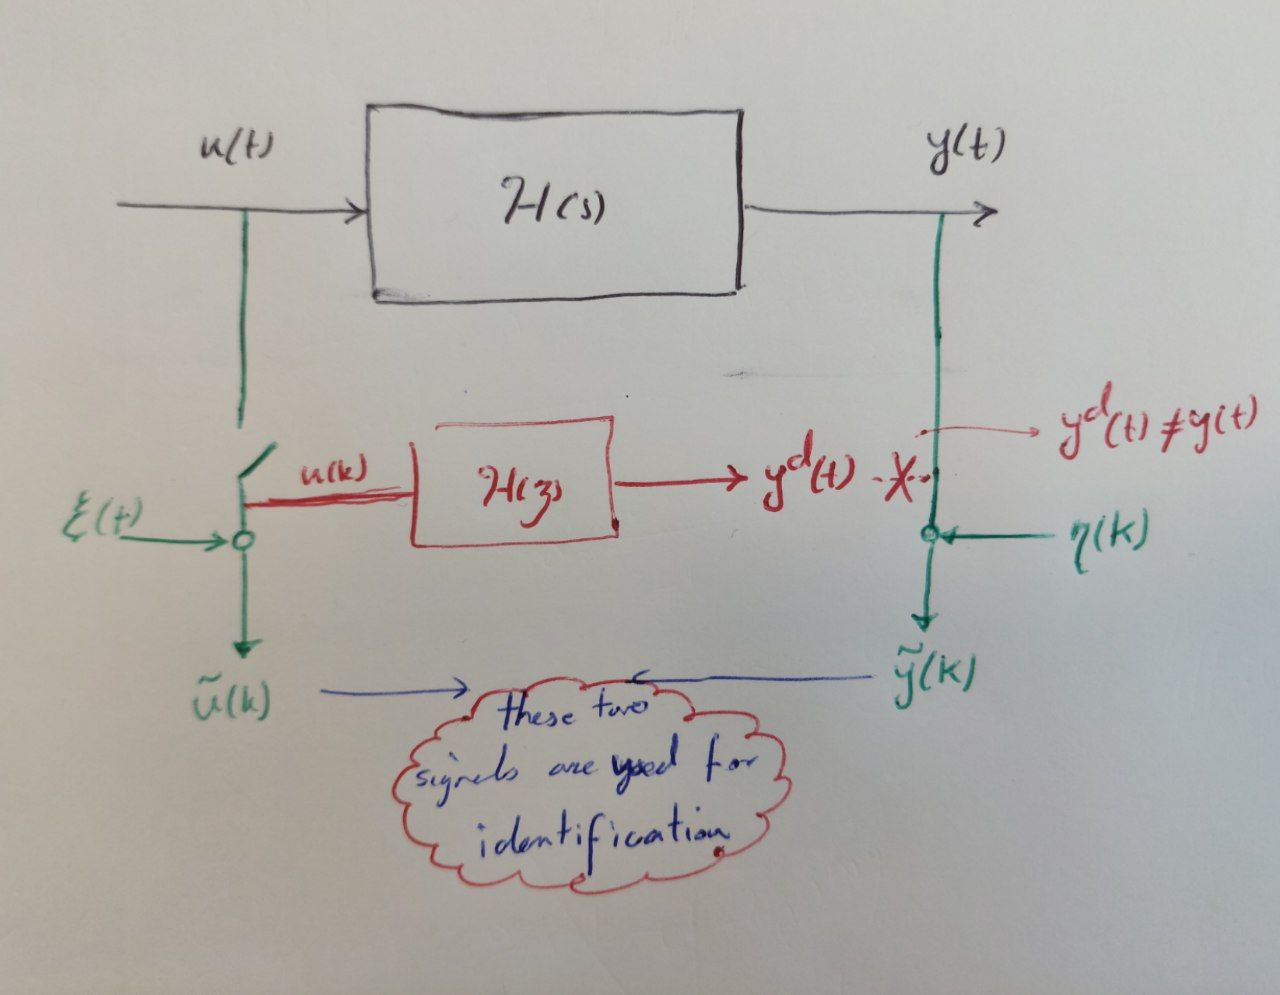
\includegraphics[width=0.75\textwidth]{images/tustin-discritization.jpg}
    \caption{scheme of the Tustin discretization set-membership identification of the continuous-time systems}
    \label{fig:FPS_time_domain}
\end{figure}

Here, 
\[
y^d(k) = H^{Tustin}(q^{-1})u(k) \neq y(k) = y(k T_s)
\]

if the assumption required by the discretization are not perfectly met.

We define
\[
\delta(k) = y^d(k) - y(k)
\]
according to set-membership framework, and we consider it as another a-priori assumption. The same as the assumption on the bound of the noise:
\[
|\delta(k)|\leq \Delta\delta
\]
\[
\begin{cases}
\delta(k) = y^d(k)-y(k)\\
\tilde{y}(k) = y(k) + \eta(k)
\end{cases}
\Rightarrow
\delta(k) = y^d(k) + \eta(k) - \tilde{y}(k)
\]
Now we introduce another component:
\[
\eta^{'}(k) \leq \Delta \eta + \Delta \delta
\]
Pay attention that $\Delta \delta$ tends to zero as $T_s \to 0$.\\
Having defined $\delta$, we can solve the problem dealing with less data, thereby solving the problem in a considerably shorter time. 

\subsubsection{Defining feasible parametric set}
\[
\mathcal{D}_\theta = \left\{ \theta \in \mathbb{R}^4 : 
\begin{aligned}
H(s) &= \frac{\beta_1 s + \beta_0}{s^2 + \alpha_1 s + \alpha_0 }, \\
\tilde{y}(k) &= y^d(k) + \eta^{'} , \quad |\eta^{'}| \leq \Delta\eta + \Delta\delta, \\
\tilde{u}(k) &= u(k) + \zeta^{'} , \quad |\zeta^{'}| \leq \Delta\zeta , \\
y^d(k) &= H(z) u(k), \quad \forall k = 1,\, 2,\, \dots,\, N
\end{aligned}
\right\}
\]

Now, we simplify $H(z)$ by multiplicating and divinding it by $Ts (z+1)^2$,
\[
H(z) = \frac{2 Ts (z+1) \beta_1(z-1) + T_s^2 (z+1)^2\beta_0 )}{4(z-1)^2 + 2\alpha_1 T_s(z-1)(z+1) + T_S^2(z+1)^2\alpha_0}
\]

\[
H(z) = \frac{2 T_S (z^2-1) +T_s^2 (z+1)^2 \beta_0}{4(z^2-2z+1) + 2\alpha_1 T_s (z^2-1) + T_s^2 \alpha_0 (z^2 + 2z + 1)}
\]

\[
H(z) = \frac{z^2(2T_s \beta_1 + T_s^2\beta_0) + z(2 T_s \beta_0) + T_s^2 \beta_1 - 2 T_s \beta_1}{z^2(4 + 2 \alpha_1 T_s + \alpha_0 T_s^2) + z(-8 + 2 T_s^2 \alpha_0) + 4 - 2 \alpha_1 T_s + T_s^2 \alpha_0}
\]

We want to reconduce the form:
\[
H(z) = \frac{\zeta_2 z^2 + \zeta_1 z + T_s^2 \zeta_0}{z^2 + \gamma_1 z +  \gamma_0}
\]

Pay attention that, in order to obtain a unique transfer function, the coefficient of the largest term in the denumerator of the transfer function should be 1. Therefore, we divide and multipli the transfer function, by the coefficient of $z^2$ in the denumerator, which is name as $a_2$, the coefficient of numerator are called $b$.\\

Now, we define the extended parameter set.

\[
\mathcal{D}_{\theta,\,\zeta,\,\gamma,\,\eta,\,\xi} = \left\{ \theta \in \mathbb{R}^4,\, \zeta \in \mathbb{R}^3,\,\gamma \in \mathbb{R}^2,\,\xi,\,\eta^{'} \in \mathbb{R}^N,\, : 
\begin{aligned}
\tilde{y}(k) &= y^d(k) + \eta^{'} , \quad |\eta^{'}| \leq \Delta\eta + \Delta\delta, \\
\tilde{u}(k) &= u(k) + \zeta^{'} , \quad |\zeta^{'}| \leq \Delta\zeta , \\
y^d(k) &= H(q^{-1},\zeta,\,\xi) u(k), \quad \forall k = 1,\, 2,\, \dots,\, N \\
\zeta_i a_2(\alpha) &= b_i(\beta), i = 0,\, 1,\,2\\
\gamma_i a_2(\alpha) &= a_i(\alpha) i = 0,\,1
\end{aligned}
\right\}
\]
The third equation is writen in implecite form to save some space, this equation should be considered in the following form:
\[
y^d(k) + \gamma_1 y^d(k-1) + \gamma_2 y^d(k-2) = \zeta_2 u(k) + \zeta_1 u(k-1) + \zeta_0 u(k-2)
\]
and considering the noise-corrupted data samples at hand:
\[
\begin{array}{c}
\tilde{y}(k) - \eta^{'}(k) + \gamma_1\tilde{y}(k-1) - \eta^{'}(k-1) + \gamma_2 \tilde{y}(k-2) - \eta^{'}(k-2) = \\ \zeta_2 \tilde{u}(k) - \zeta_2 \xi(k) +\zeta_1 \tilde{u}(k-1) - \zeta_1 \xi(k-1) + \zeta_0 \tilde{u}(k-2) - \zeta_0 \xi(k-2)
\end{array}
\]

\[
\underline{\theta}_i = \arg \min_{\substack{(\theta, \gamma, \xi, \eta', \zeta) \\ \in \mathcal{D}_{\theta, \gamma, \xi, \eta', \zeta}}} \theta_i
\]

\[
\overline{\theta}_i = \arg \min_{\substack{(\theta, \gamma, \xi, \eta', \zeta) \\ \in \mathcal{D}_{\theta, \gamma, \xi, \eta', \zeta}}} -\theta_i
\]

Finally, we recognize that $\zeta_i a_2(\alpha)$ and $\gamma_i a_2(\alpha)$ are in $\theta,\,\zeta,\,\gamma$ and the problem of computing PUI on $\alpha,\,\beta$ is a POP.

\subsubsection{Remarks about this approach}
\begin{itemize}
    \item If we assumed $\Delta\delta = 0$ and we use noise-free data; then, the problems of finding the PUIs might become \textbf{infeasible}, due to assuming a strong a-priori assumption.
    \item Notice that \textbf{the bound on the discretization error} must be provided as an a-priori assumption, but \textbf{it depends on the sampling rate $T_s$ and on the input signal.}\\
    a possibility is to estimate $\Delta\delta$ from the available data as follows: we try to solve the following problem until we obtain a feasible solution:\\
    \[
    \Delta^{*}_\delta = \arg \min \Delta_\delta \text{  s.t  } 
    \begin{aligned}
\tilde{y}(k) &= y^d(k) + \eta^{'} , \quad |\eta^{'}| \leq \Delta\eta + \Delta\delta, \\
\tilde{u}(k) &= u(k) + \zeta^{'} , \quad |\zeta^{'}| \leq \Delta\zeta , \\
y^d(k) &= H(q^{-1},\zeta,\,\xi) u(k), \quad \forall k = 1,\, 2,\, \dots,\, N \\
\zeta_i a_2(\alpha) &= b_i(\beta), i = 0,\, 1,\,2\\
\gamma_i a_2(\alpha) &= a_i(\alpha) i = 0,\,1
\end{aligned}
    \]
    However, there is no guaranatee that $\Delta_\delta^{*}$ will  be larger than the true bound on the discretization error. 
\end{itemize}






\chapter{Enforcing stability of the model}
The topic of this chapter is how to enforce stability of the identified models.\\

Every time we perform an open-loop experiment, it is required that the system is BIBO stable. Otherwise, given a bounded input \( u(k) \), the output \( y(k) \) might diverge, and we would not be able to measure it. Physically, the system would be destroyed. 

The fact that a system is BIBO stable is a \textbf{strong indication} of the parameters! Therefore, adding this information to the problem allows for more \textbf{accurate} estimates, which means smaller PUIs in our SM identification context.\\

\section{Stability of a discrete-time LTI system}
The following statements are equivalent:
\begin{enumerate}
    \item \( G_p(z) = \frac{N(z, \theta)}{D(z, \theta)} \) is BIBO stable:
    
    \item \( D(z, \theta) \neq 0 \)   for all \( z \in \mathbb{C} \) such that \( |z| \geq 1 \).\\
    
    \textbf{Observation:} We note that stability depends only on the parameters appearing in the denominator, which in turn defines the poles of the system.
    \newpage
    \item \textbf{Jury's theorem}:\\
    Let's define the Jury array as follows: \\
    
    Given \( D(z,\theta) = 1 + a_1 z^{-1} + a_2
    z^{-2} + \cdots + a_n z^{-n} \), the Jury array is defined by:

\[
\begin{array}{*{7}{c}@{\hspace{10pt}}}
    a_n & a_{n-1} & a_{n-2} & \cdots & a_2 & a_1 & a_0 = 1 \\
    1 & a_1 & a_2 & \cdots & a_{n-2} & a_{n-1} & a_n \\
    c_{n-1} & c_{n-2} & c_{n-3} & \cdots & c_1 & c_0 &  \\
    c_0 & c_1 & c_2 & \cdots & c_{n-2} & c_{n-1} &  \\
    d_{n-2} & d_{n-3} & \cdots & d_1 & d_0 & & \\
    d_0 & d_1 & \cdots & d_{n-3} & d_{n-2} & & \\
    \vdots & \vdots & \vdots & \vdots &  &  &  \\
    q_2 & q_1 & q_0 & & & & 
\end{array}
\]


    where:
    \[
    c_{n-1} = \det\left( \begin{bmatrix}
        a_n & a_{n-1} \\
        1   & a_1
    \end{bmatrix} \right)
    \]
    \[
    c_{n-2} = \det\left( \begin{bmatrix}
        a_n & a_{n-2} \\
        1   & a_2
    \end{bmatrix} \right)
    \]
    and,
    \[
    d_{n-2} = \det\left( \begin{bmatrix}
        c_{n-1} & c_{n-2} \\
        c_0   & c_1
    \end{bmatrix} \right)
    \]
   \[
    d_{n-3} = \det\left( \begin{bmatrix}
        c_{n-1} & c_{n-3} \\
        c_0   & c_3
    \end{bmatrix} \right)
    \]

    in general,
           \[
    c_{n-j} = \det\left( \begin{bmatrix}
        a_n & a_{n-j} \\
        a_0 =1   & a_j
    \end{bmatrix} \right)
    \]
    and
         \[
    d_{n-j} = \det\left( \begin{bmatrix}
        c_{n-1} & c_{n-j} \\
        c_0   & c_{j-1}
    \end{bmatrix} \right)
    \]
    
    Visually, it can be seen in the following figure.
    \begin{figure}[H]
    \centering
    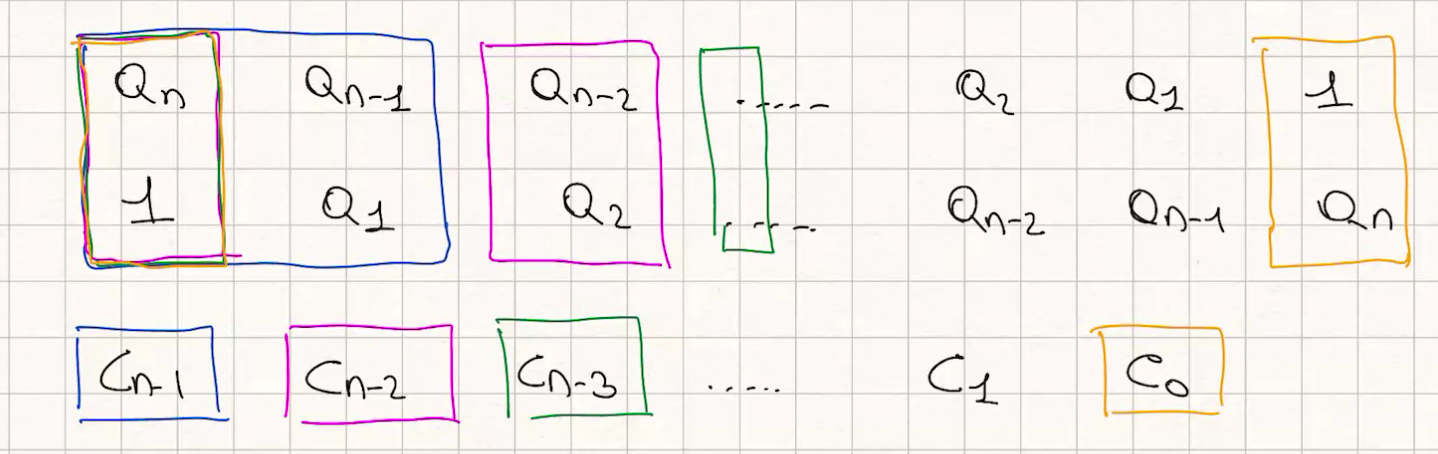
\includegraphics[width=0.75\textwidth]{jury-array.png}
    \caption{Shaping the third row of the Jury array of the aforementioned polynomial}
\end{figure}

    \textbf{Theorem (Jury)}:\\
    The roots of the polynomial $D(z,\theta)$ belongs to the open unit circle, which mathematically means \( D(z, \theta) \neq 0 \)   for all \( z \in \mathbb{C} \) such that \( |z| \geq 1 \), if and only if the following equations hold:
    \begin{itemize}
        \item\(
    D(z=1) = 1 + a_1 + a_2 + \cdots + a_n > 0
    \) 
        \item \((-1)^n D(z=-1) = (-1)^n (1 - a_1 + a_2 - a_3 + \cdots \pm a_n) >0\) 
        \item \(|a_n|<1 \)
        \item \(|c_{n-1}|< |c_0| \)
        \item \(|d_{n-2}| < |d_0|\)\\
        \vdots
        \item \(|q_2| < |q_0|\)
    \end{itemize}
    The first three inequalities are in $\theta$, while the others ones depending on the Jury array, can become non-linear, since we are dealing with the absolute values. In order to reformulate the problem in a form that can be handled in a linear fashion we adopt the following trick.
      \begin{itemize}
        \item \((c_{n-1})^2< (c_0)^2 \)
        \item \((d_{n-2})^2 < (d_0)^2\)\\
        \vdots
        \item \((q_2)^2 < (q_0)^2\)
    \end{itemize}
    These constraints now become \textbf{quadratic non-convex inequalities} in the elements of the Jury arrya. Moreover, the elements of the Jury array are \textbf{polynomial functions of $\theta$}, or at any rate we are dealing with determinent of two by two matricies, which leads to bilinear equations of the elements of the matrix.\\
    to conclude:
    \begin{itemize}
    \item We can enforce stability of the identified model by, \textbf{adding optimization variables representing the entried of the Jury array}, $c_{n-1},c_{n-2},\cdots,c_0,d_{n-2},\cdots,q2,q0 $, the definition of $q_1$ is not needed. Now we can modify the EFPS to include the:
     \item relations between $\theta$ and the entried of the Jury array \(a_1,\cdots,a_n \rightarrow c_{n-1},\cdots,c_0\)\\
     \item relations between different entried of the Jury array  \(c_{n-1},\cdots,c_0 \rightarrow d_{n-2},\cdots,d_0\) and so on up to $q_2$ and $q_0$\\
     \item Now, the equations from the Jury theorem.
    \end{itemize}
    \textbf{Remark:} even if we include these constraints, there is no guarantee that the final identified model will be stable, for the following reasons:
    \begin{itemize}
        \item we relax our POPs to convex SDP:
     \begin{figure}[H]
    \centering
    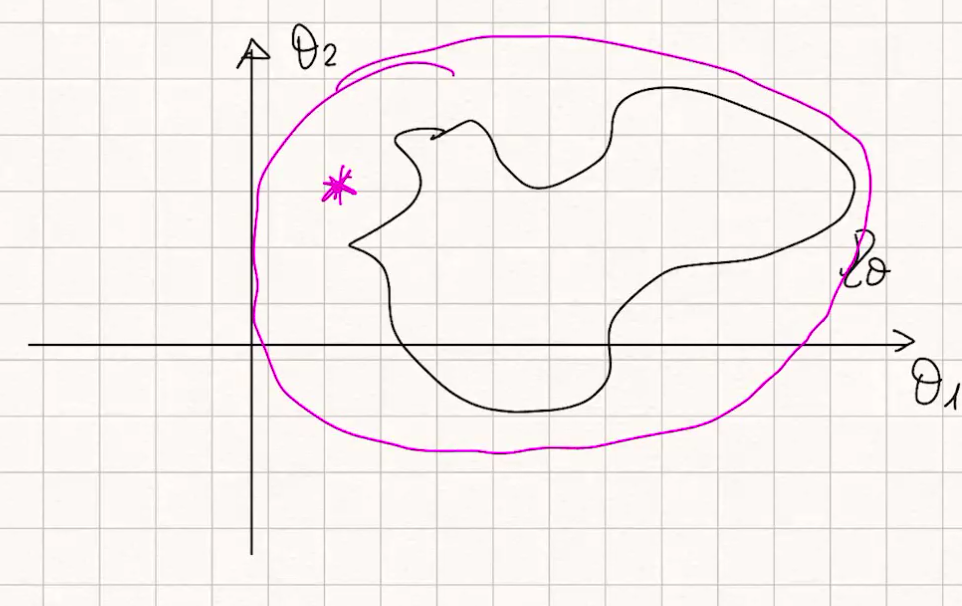
\includegraphics[width=0.75\textwidth]{SDP-convex-set.png}
    \caption{Since we relax our problem, the model obtained showed by * does not satisfies the stability property, since it does not satisfies all the constraints.}
\end{figure}
    \item Even if we could describe the exact FPS, then when taking the central estimate, we may \textbf{fall out of} the set, because our FPS is non-convex.
    \begin{figure}[H]
    \centering
    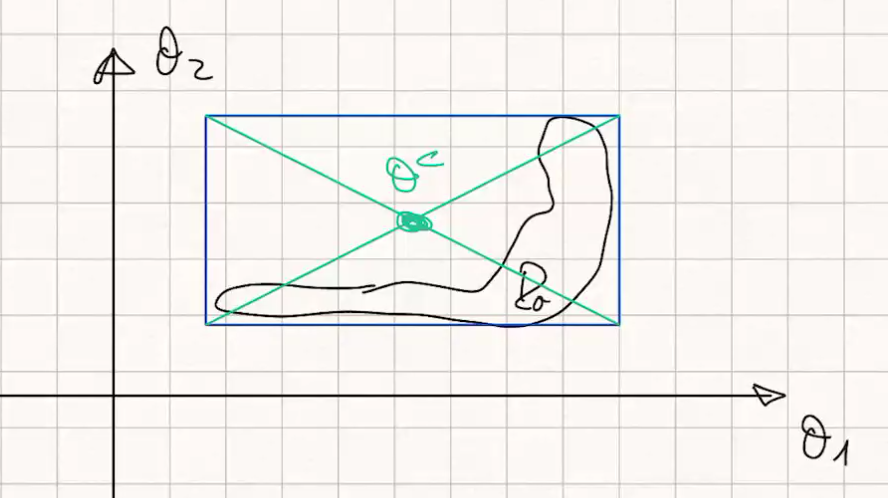
\includegraphics[width=0.5\textwidth]{centra-estimate.png}
    \caption{The central estimate that does not fall into the FPS.}
\end{figure}
    \end{itemize}
    So why enforcing stability constraints? since they shrink the FPS and ultimately improve the accuracy of the model because the obtained PUIs will be smaller.
\end{enumerate}

\begin{example}
\[
H(z) = \frac{\beta_1 z^{-1}}{1 + a_1 z^{-1} + a_2 z^{-2} + a_3 z^{-3}}
\]
we have the following Jury constraints
\[
D(z=1)> 0 \Rightarrow 1 + a_1 + a_2 + a_3 > 0
\]
\[
(-1)^nD(z=-1)> 0 \Rightarrow -1 + a_1 - a_2 + a_3 > 0
\]
\[
-1 <a3< 1
\]
Now, we need to shape Judy table, we need to go up to the third row, since the row with three element becomes the third row.
\[
\begin{array}{*{4}{c}@{\hspace{10pt}}}
    a_3 & a_2 & a_1 & 1 \\
    1 & a_1 & a_2 & a_3 \\
    c_2 & c_1 & c_0  
\end{array}
\]
where 
\[
c_2 = a_3 a_1 - a_2
\]
as it was mentioned $c_1$, here, is not needed.
\[
c_0 = a_3 a_3 - 1
\]
Now,
\[
|c_2|<|c_0| \Longleftrightarrow c_2^2 <c_0^2
\]

\end{example}


















\chapter{Direct Data-Driven Control design}
\section{introduction}

In this chapter a new approach for designing controllers is going to be adopted. In general for designing controllers we have the following situations:
\begin{itemize}
    \item \textbf{Model-based controller design}: in this case, the model of the system is known and is used to design the controller in a convensional manner.
    
    \item \textbf{Data-Drive controller design}: here, the model of the system is obtained using experimental data, by means of SM identification for instance. Afterwards, the model is used in order to design the controller.
    
    \item \textbf{Direct Data-Driven controller design}: In this method, there is no need for an intermediate step of identifying the model of the system. In this appraoch, the controller is designed without knowing the model of the system and just by using the experimental input-output data.
    
\end{itemize}

In this chapter the third case is going to be discussed. The scheme we considere here is as follows: 
 \begin{figure}[H]
    \centering
    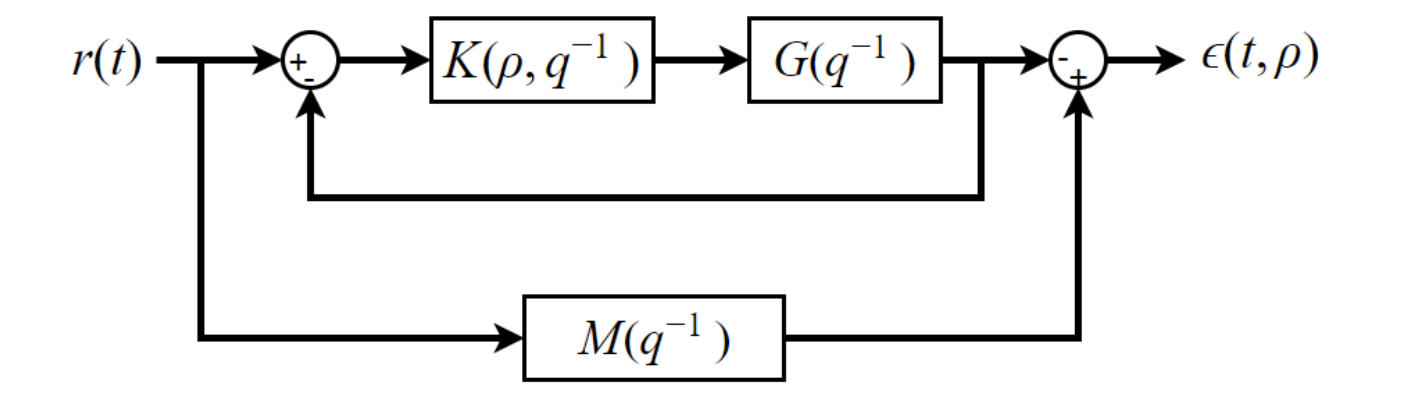
\includegraphics[width=0.75\textwidth]{dddc-scheme.png}
    \caption{Feedback control system to be designed compared with the
 reference model $M(q^{-1})$}
 \end{figure}
In this scheme, $M$ represents the \textbf{reference model}, the resultant control system, which is expected to satisfy the requirements, and $G$ is the unknown plant to be controled. 


\section{DDDC design procedure}
\subsection{Task 1: to find the controller}
The first task is to find a controller $K(\rho,\,q^{-1})$ - $K$ is an LTI discrete-time system with a transfer function depending on some parameter $\rho$ - such that the complementary sensitivity function of the controller,$T$, is close enough to the transfer function of the reference model $M$.

\[
T(q^{-1}) \approx M(q^{-1})
\]
\[
T(q^{-1}) = \frac{G(q^{-1}) K(\rho,q^{-1})}{1+G(q^{-1}) K(\rho,q^{-1})}
\]

In this equation, ideally, we expect equality for the equation above. Therefore, we are seeking to find $K$ such that:

\[
M =  \frac{G(q^{-1}) K(\rho,q^{-1})}{1+G(q^{-1}) K(\rho,q^{-1})}
\]

This problem is called, \textbf{\textit{Model matching problem}}.

\subsubsection{Result 1}
If $G(q^{-1})$ is known, the model-based matching problem has a trivial solution, which provides what we called the \textit{"ideal controller $K^{*}$"}:
\[
M + MGK = GK \Rightarrow K^{*} = \frac{M}{(1-M)G}
\]

\subsubsection{Result 2}
It can easily be shown that the ideal controller $K^{*}$
\begin{itemize}
    \item can be physically unrealisable, because the order of the denuminator of the $K^{*}$ may be large than that of the numerator. This, however, can be overcomed by suitablly adding high frequency poles.
    \item $K^{*}$ is not guaranteed to provide internal stability of the feedback control system, because $K^{*}$ is, in general, performing unstable zero-pole cancellation in $G$, which means cancelling of poles with a norm larger than 1.
\end{itemize}

\subsubsection{Result 3}
It is possible to prove that $K^{*}$ is ensuring internal stability if and only if the transfer function $M(q^{-1})$ includes all the unstable zeros of $G(q^{-1})$. \\

\subsubsection{Result 4}
Result 3 allow us to fix the second problem, to save internal stability, but what what we pay is that the modified $M(q^{-1})$ that will include het "unstable" zeros is no more a descriptoin of the describe behavior.\\

\subsubsection{Result 5}
We are assuming that $G$ is not known. Then, we can collect input-output data by performing an experiment on the plant, and we calculate the error transfer function $E$. Ideally, $E$ is zero.

\begin{factbox}
Pay attention that, here, the system $G$ must be BIBO stable so that we can perform an open-loop experiment, so the system have poles with a norm strictly smaller than 1. 
\end{factbox}

\[
E = M - \frac{G(q^{-1}) K(\rho,q^{-1})}{1+G(q^{-1}) K(\rho,q^{-1})}
\]
Here, $G$ is unknown, and $K$ is to be designed. This equation is in terms of systems and not the system output. Now, let's apply to both terms teh signal $r(t)$. By doing so, we are changing our problem to system output rather than the system. However, we have to assume that this equation can be solve for all the referecen signal.
\[
Mr =  \frac{G(q^{-1}) K(\rho,q^{-1})}{1+G(q^{-1}) K(\rho,q^{-1})}r \:\:\: \forall r(t)
\]
Here, the left side of the equation is the output of $M$ when the input $r$ is applied, and the right side of the equation is the output of the feedback control system when the same input is applied. Therefore,
\[
\mathcal{E}(t) = M.r - \frac{G(q^{-1}) K(\rho,q^{-1})}{1+G(q^{-1}) K(\rho,q^{-1})}r \:\:\: \forall r(t)
\]
where $\mathcal{E}(t)$ is the output error signal.Ideally, it should be zero for all $t$ and $r(t)$, or at any rate, it is our task.

\[
\begin{array}{c}
\mathcal{E}(t) = 0 \\
\Updownarrow \\
Mr - MKGr = KGr \\
\Updownarrow \\
(1-M)KGr = Mr\\
\Updownarrow \\
KGr = \frac{M}{1-M}
\end{array}
\]
\begin{factbox}
Pay attention that $E$ is the system error, while $\mathcal{E}(t)$ is the output error signal.
\end{factbox}

It can be seen that this equation still depends on $G$, which is not known. By replacing $Gr$ with the signal $y$.\\

Now, by simulation, considering the right-hand side of the equation, we can obtain a signal which is defined in the following manner:
\[
s(t) = \frac{M}{1-M} r(t)
\]
now, we can use the following equation for deriving the controller.
\[
K(\rho,q^{-1}) .y(t) = s(t)
\]

Finally, since through the experiment, we can obtain $\tilde{y}(k)$, so by replacing it in the equation we obtain.
\[
s(k) = K(\rho,q^{-1})[\tilde{y}(k) - \eta(k)]
\]
 \begin{figure}[H]
    \centering
    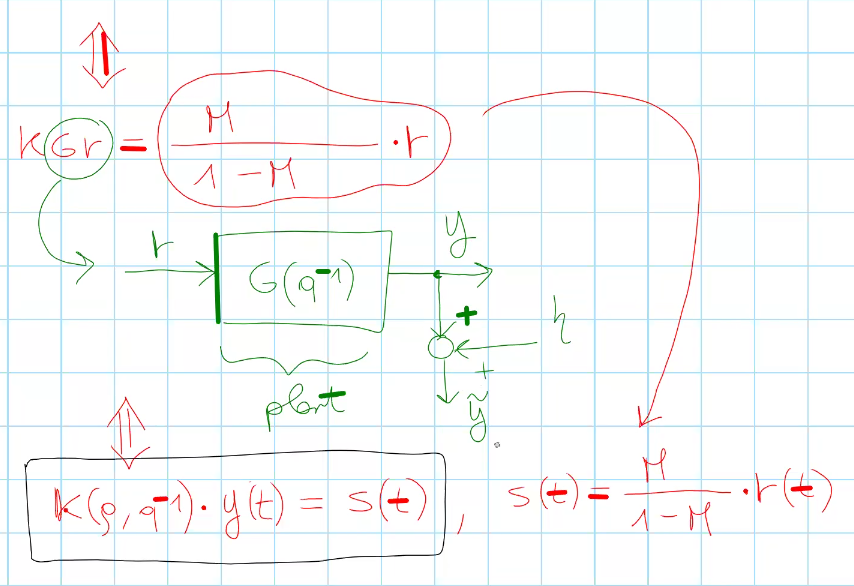
\includegraphics[width=0.65\textwidth]{dddc-prof-sketch.png}
    \caption{A graphical representation of the reasoning behind this manipulation.}
 \end{figure}
The problem of designing $K$ is infact an input-error System-identification problem under the assumption that:
\[
|\eta(k)|<\Delta\eta \:\:\: \forall k
\]
Which is a particular case of the EIV set-membership input-output problem. In order to solve ethe SM identification problem we need to select the \textbf{class of controller $C$}. e.g:
\[
C = \{\text{class of PID controllers}\}
\]
or
\[
C = \{\text{class of LTI controllers of fixed and given order}\}
\]

\textbf{How to check if $C$ is a "good" controller class?}\\
The next step in set-membership approach is to define the \textit{\textbf{Feasible Controllers Parameter set (FCPS)}}.
\[
\mathcal{D}_\rho = \{
\rho \in \mathbb{R}^{\text{length of $rho$}}: s(k) = K(\rho,q^{-1})[\tilde{y}(k) - \eta(k)],\,|\eta(k)|<\Delta\eta,\,\forall\,\,t = 1,\,2,\,\cdots,\,N
\}
\]
and then, since the description of the set is not explicit, what we do is to consider \textbf{\textit{Extended Feasible Controller Parameter Set}}, EFCPS.
\begin{example}[an example]
consider
\[
C = \{\text{class of first-order LTI controllers}\} = {K = \frac{\rho_2 + \rho_3 q^{-1}}{1 + \rho_1 q^{-1}}}
\]
for this case, FCPS becomes
\[
\mathcal{D}_\rho = \{
\rho \in \mathbb{R}^{3}: s(k) + \rho_1s(k-1) = \rho_2[\tilde{y}(k) - \eta(k)] + \rho_3[\tilde{y}(k-1) - \eta(k-1)],\,|\eta(k)|<\Delta\eta,\,\forall\,\,k = 2,\,\cdots,\,N
\]
and EFCPS becomes
\[
\mathcal{D}_{\rho,\,\eta} = \{
\rho \in \mathbb{R}^{3},\eta \in \mathbb{R}^N : s(k) + \rho_1s(k-1) = \rho_2[\tilde{y}(k) - \eta(k)] + \rho_3[\tilde{y}(k-1) - \eta(k-1)],\,|\eta(k)|<\Delta\eta,\,\forall\,\,k = 2,\,\cdots,\,N
\]
\end{example}

\textbf{Important Remark}: If $\mathcal{D}_{\rho,\,\eta}$ is empty, there is no controller in the considered class $C$ which solves the controller design problem.


\subsubsection{Result 6}
$\mathcal{D}_{\rho,\eta}$ is empty if and only if at least one of the POPs to be solved for computing the \textbf{\textit{controller parameter uncertainty intervals (CPI)}} is infeasible, which means negative exit flag in sparsepop command.
 

\subsubsection{Summerizing the controller design procedure:}
\begin{enumerate}
    \item Perform an experiment applying the reference signal $r(t)$to the plant and collect the output:
    \[
    \tilde{y}(k) = y(k) + \eta(k),\,|\eta(k)| < \Delta\eta
    \]
    
    \item Build FCPS and EFCPS
    \item compute the CPUI:
    \[
    \text{CPUI}_i = [\:\underline{\rho},\:\overline{\rho}\:]
    \]
    where
    \[
    \underline{\rho}_i = \min\limits_{\rho,\eta \in \mathcal{D}_{\rho,\,\eta}} \rho_i
    \]
    \[
    \overline{\rho}_i = \max\limits_{\rho,\eta \in \mathcal{D}_{\rho,\,\eta}} \rho_i
    \]
    \item If one of the problems is infeasible, \textbf{we have to update our controller class $C$}, which will be discussed later.
    If, on the contrary, all the POPs are feasible (positive exit flag), we obtain the CPUI for all $\rho_i$.
    \item Build the controller transfer function as:
    \[
    K(\rho,q^{-1}) = \frac{\rho_{n+1}^c + \rho_{n+1}^cq^{-2} + \cdots + \rho_{2n+1}^cq^{-n}}{1+ \rho_1^cq^{-1} + \rho_2^cq^{-2} \cdots + \rho_{n}q^{-n}}
    \]
    where $\rho_i^c$ is the Chebyshev center of the parameter $i$.
\end{enumerate}

\subsubsection{Result 7}
If $K^{*} \in C$, then $K^{*} \in \mathcal{D}_\rho$
 \begin{figure}[H]
    \centering
    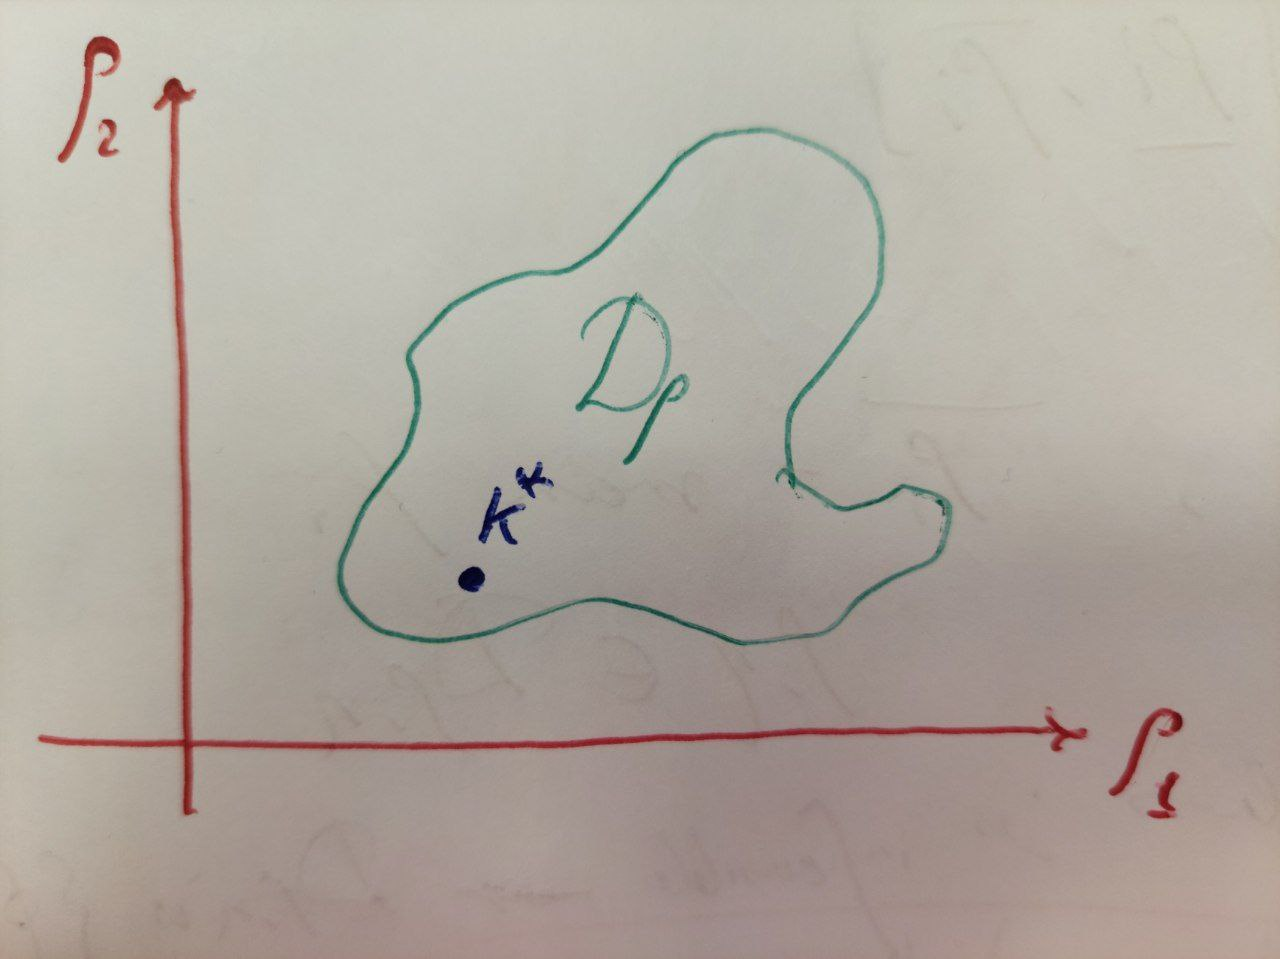
\includegraphics[width=0.65\textwidth]{d-rho.jpg}
    \caption{Feedback control system to be designed compared with the
 reference model $M(q^{-1})$}
 \end{figure}


\subsubsection{Result 8}
Since we don't know $K^{*}$, if we assume that $K^{*} \in \mathcal{D}_\rho$, the worst-case estimation of $K^{*}$ is going to be for a K on the boundary of $\mathcal{D}$ with the largest distance, so we choose $K$ to be $K(\rho^c,q^{-1})$, where
\[
\rho^c = \arg \min_{\rho \in \mathbb{R}^{\text{length of $\rho$}}} \max_{\rho' \in \mathcal{D}_\rho} \|\rho - \rho'\|_\infty
\]

considering $l_\infty$ for our cost function, $\rho^c$ becomes the Chebyshev center of the FCPS.


\subsubsection{Result 9}
It possible that the Chebyshev center in the $l_\infty$ norm is given by:
\[
\rho^c = \frac{\underline{\rho}+\overline{\rho}}{2}
\]
Since in $l_\infty$ we are considering a box around our $\mathcal{D}$ so the center of this box becomes the mean of the CPUIs.

Now, the procedure for the controller class is as follows. First, a first order model is chosen, then if it weren't feasible, the degree is increased, until we find a feasible solution.

\subsection{Considerations regarding the reference signal}
In the previous discussion, we were able to eliminate the transfer function $G(q^{-1})$ from the equation by applying the reference signal to both sides of the equation 
\[
\begin{array}{c}
\begin{cases}
E(\rho,q^{-1}) = 0\\
E(\rho,q^{-1}) = M(q^{-1}) - \frac{K(\rho,q^{-1})G(q^{-1})}{1 + K(\rho,q^{-1})G(q^{-1})}
\end{cases}
\Rightarrow M(q^{-1}) - \frac{K(\rho,q^{-1})G(q^{-1})}{1 + K(\rho,q^{-1})G(q^{-1})} = 0\\
 \Updownarrow\\
 \mathcal{E} = 0 \Leftrightarrow s(t) = K(\rho,q^{-1})\left[\tilde{y}(t)- \eta(t)\right] \:\:\:\: \forall r(t)
\end{array}
\]
And the last one should be true for all the reference signal $r$. It means that in order to try, practically, to force that equation
\[
 s(t) = K(\rho,q^{-1})\left[\tilde{y}(t)- \eta(t)\right] 
\]
is satisfied for all $r(t)$, we have to select $r(t)$ to be used in the experiment as a white noise, because \textbf{by definition as white signal is a signal having a flat spectrum at all frequencies,} which means such a signal applied to the plant is able to excite the system dynamics as well as any other signal.

\begin{factbox}[Dicussion regarding the reference signal]
If we apply a step reference signal, we are not exciting all the possible dynamics of the system, because of the spectrum of the step signal. The reason this is true is that the essential content of a step signal is the dc-gain of the signal, frequency equal to 0.\\
 \begin{figure}[H]
    \centering
    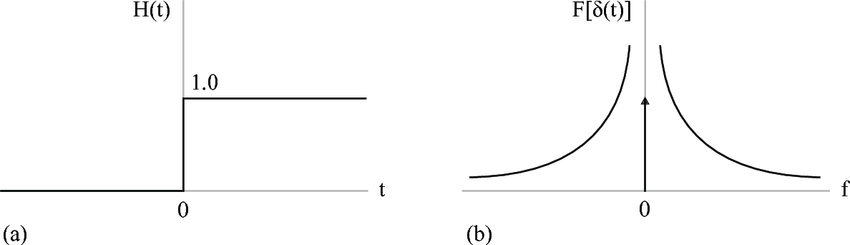
\includegraphics[width=0.65\textwidth]{step-spectrum.png}
    \caption{The frequency spectrum of step signal function}
 \end{figure}
 
 On the other hand, using a sinusoidal signal with a specific frequency stimulates the system exactly at that frequency; again you can consider the frequency response of the sinusoidal signal.\\
 
 \end{factbox}
 \begin{factbox}
 \textbf{In the procedure of designing a data-driven controller, if we pick the step reference signal, we can only say that the controller we are willing to design will be able to match the behavior of the reference system when the reference system is a step signal}. In this case, if we apply a different reference signal - for example, a sinusoidal reference signal with a high frequency - it is not guaranteed that the control system is going to match that of the reference model when that signal is applied to it.
 
In order to be able to cover all situations, in practice, we have to perform a large number of experiment considering all the signals that are of interest in our application. Afterwards, we have to collect all the data that we have obtained by different experiements. Finally, we should perform the identification using all the collected data.\\

Alternatively, if we don't know which signal is going to be used, we can use a white-noise signal to excite the plant. 

\end{factbox}


\subsection{Standard approach for selecting/designing the reference model $M_r(q^{-1})$(Not included in the exam)}
The reference model $M_r(q^{-1})$ is typically selected in order to impose a certain desired behavior to the complementary sensitivity function $T(q^{-1})$ of the feedback control system to be designed.

\begin{example}[Examples]
We can select $M_r(s)$ (continuous-time reference model) by looking at the desired step response of the feedback control system. \\

\textbf{Example 01}: to obtain a response that has the following shape,
\[
M_r(s) = \frac{1}{1+ \frac{s}{p}}, \:\:\: p > 0 
\]
which has the behavior of a stable first-order system that has a dcgain equal to 1, in order to enforce tracking the reference signal at the steady-state condition. By tuning $p$, the speed of the response can be changed.\\

\textbf{Example 02}:
A reference model that has the behavior of a second-order system.
\[
M_r(s) = \frac{\omega_n^2}{s^2 + 2 \zeta \omega_n s + \omega^2}
\]
\end{example}

\textbf{The limitation of this approach} is that by only selecting $M_r(s)$ in view of the design response of $T$, we can only impose the behavior of the feedback control system from the point of view of the reference tracking performance to one or more reference signals, but the behavior of the feedback control system as well as the attenuation of distrubrances and/or sensor noise is concerned, it is almost out of our control. \\

In fact, once we have selected $M_r(s)$ as in the previous two examples, we can obtain $M_r(q^{-1})$ by discretizing $M_r(s)$. However, the response to the disturbance $d_p$ at the output, as an example, is related to the sensitivity function of the feedback control system, which is 
\[
S(q^{-1}) = 1 - T(q^{-1})
\]
In case our desired data-driven controller is going to match exactly $M_r(q^{-1})$\\
\[
S(q^{-1}) = 1 - T(q^{-1}) = 1 - M_r(q^{-1})
\]
Nonetheless, it is not guaranteed at all that the resultant $S(q^{-1})$ is going to enjoy good attenuation property with respect to the output disturbance $d_p$ acting on the output.\\

\subsubsection{Idea (proposed approach)}
The idea is to design $M_r(q^{-1})$ by solving a \textbf{\textbf{"ficticious control design problem"}} accounting for all the quantitative performance requirements involved in the considered control problem. Here, we are refering to the following problem:\\

Assuming that our real task in a real control problem is, given a plant $G$, we want to desing a controller $K$ such that the controller have the following classes of quantitative performance requirements that accounts for:
\begin{itemize}
    \item steady-state response to polynomial reference inputs $r$
    \item steady-state response to polynomial distrubance $d_p$ 
    \item steady-state response to measurement disturbances $d_s$
    \item transient step response requirements on overshoot $\hat{s}$
    \item rise time $t_r$ and settling time $t_s$
\end{itemize}

 \subsubsection{Reference model desing in DDDC method}
 The problem addressed in the paper is to design the reference model $M$ such that the DDDC system designed on the basis of such a model meets classes of quantitative performance specifications listed above.
 
 \begin{figure}[H]
    \centering 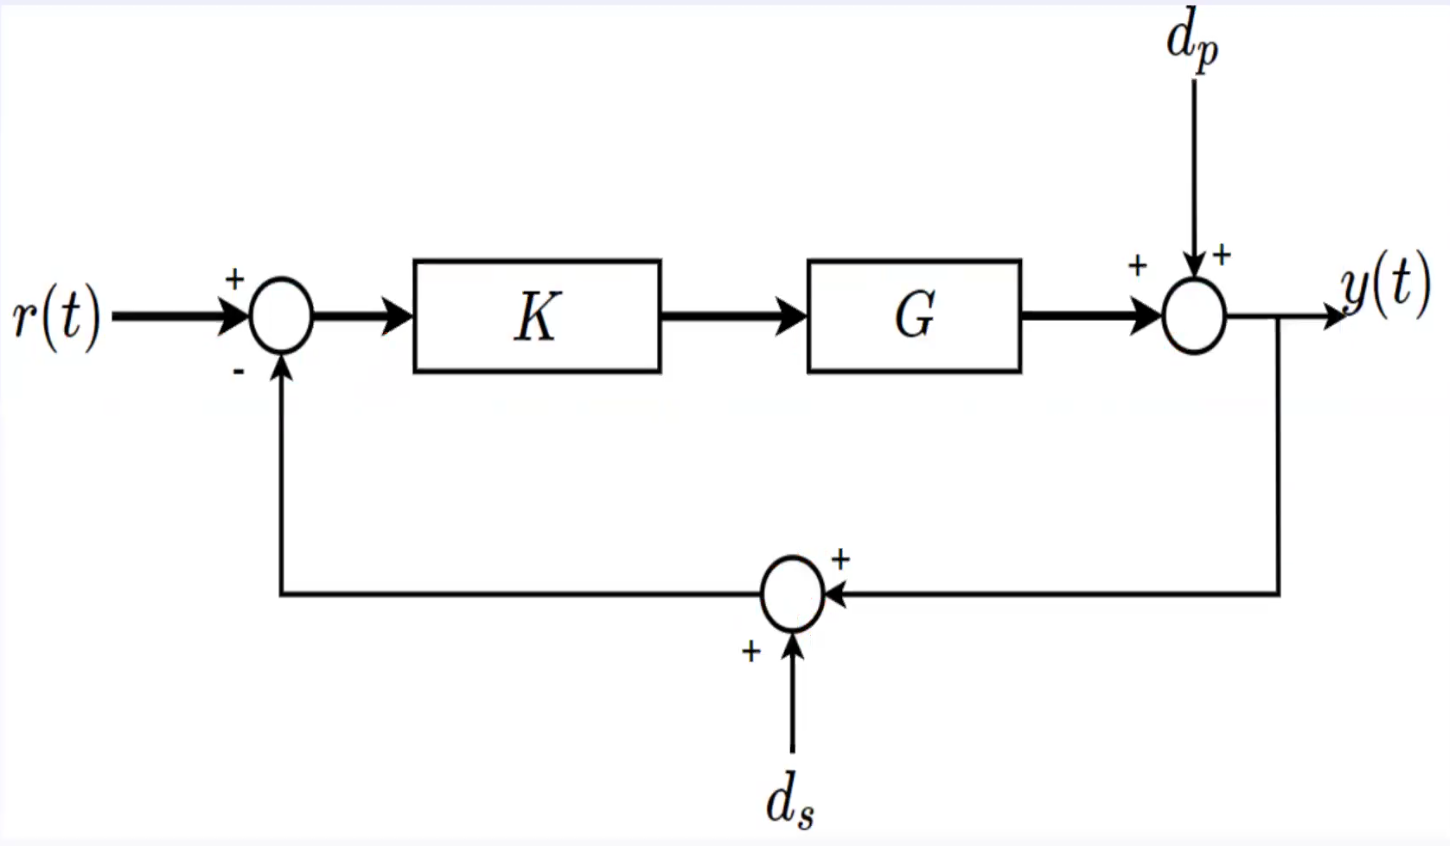
\includegraphics[width=0.65\textwidth]{fic-control-problem.png}
    \caption{The scheme of the ficticious control problem to be considered.}
 \end{figure}
 
 \subsubsection{The proposed approach}
\textbf{ I) }The main idea is that the reference model $M_r(q^{-1})$ that we are going to select will play the role of the ideal complementary sensitivity function $T(q^{-1})$ of the feedback control system. Therefore, by selecting $M_r(q^{-1})$, we can impose the reference tracking performance, but also the performance related to the attenuation of the sensor noise $d_s$.\\
 
 \textbf{II)} At the same time,  the performance related to the attenuation of the output disturbance $d_p$ depends on the shape of \\
 \[
 S(q^{-1}) = 1 - T(q^{-1}) = 1 - M_r(q^{-1})
 \]
 I and II are true since, in a feedback control system that we are considering\\
 \[
 y = T.r + Sd_p + Td_s
 \]
 If the plant $G$ is known, we can adopt any control design technique in order to design the controller. However, here, we don't know $G$. \\
  
 At this step, we don't want to obtain the controller, and, by the way, it is not possible at this stage. Now, we want to design the function $T$ and $S$ such that they satisfy the specified requirements.\\

\subsubsection{How to select the ficticious plant}
\begin{enumerate}
    \item If the true $G$\textbf{ does not have} \textit{non-minimum-phase zero} - zeros our of the unit circle:\\
    In this case, we consider a $G_{\text{ficticious}} = 1$.\\
    \begin{QandAbox}
    Because our aim at this stage is just to find what is the reference model to be obtained such that if the reference model is equal $T$, and in turn the sensitivity function $S = 1 - T$, all the requirements are satisfied. Since the behavior of the closed loop system only depends on $T$ and $S$.
     \[
 y = T.r + Sd_p + Td_s
 \]
  Then, we obtain a ficticious controller $K_{\text{ficticious}}$ that is able to control the ficticious plant satisfying the requirements. \textbf{As a result}
  \[
  T = \frac{K_{\text{ficticious}}G_{\text{ficticious}}}{1 + K_{\text{ficticious}}G_{\text{ficticious}}}
  \]
  Then, we use this $T$ for our direct-data-driven-controller problem so as to obtain the controller for the actual plant. \textbf{Since the resultant controller for the actual plant is going to result in a complementary sensitivity function $T = M_r$}, we are sure that the requirements are going to be satisfied.
    \end{QandAbox}
    \begin{example}[$H_\infty$ technique for designing the reference model (solving the ficticious control problem)]
    Condiring $H_\infty $ technique for designing the controller
     \begin{figure}[H]
    \centering 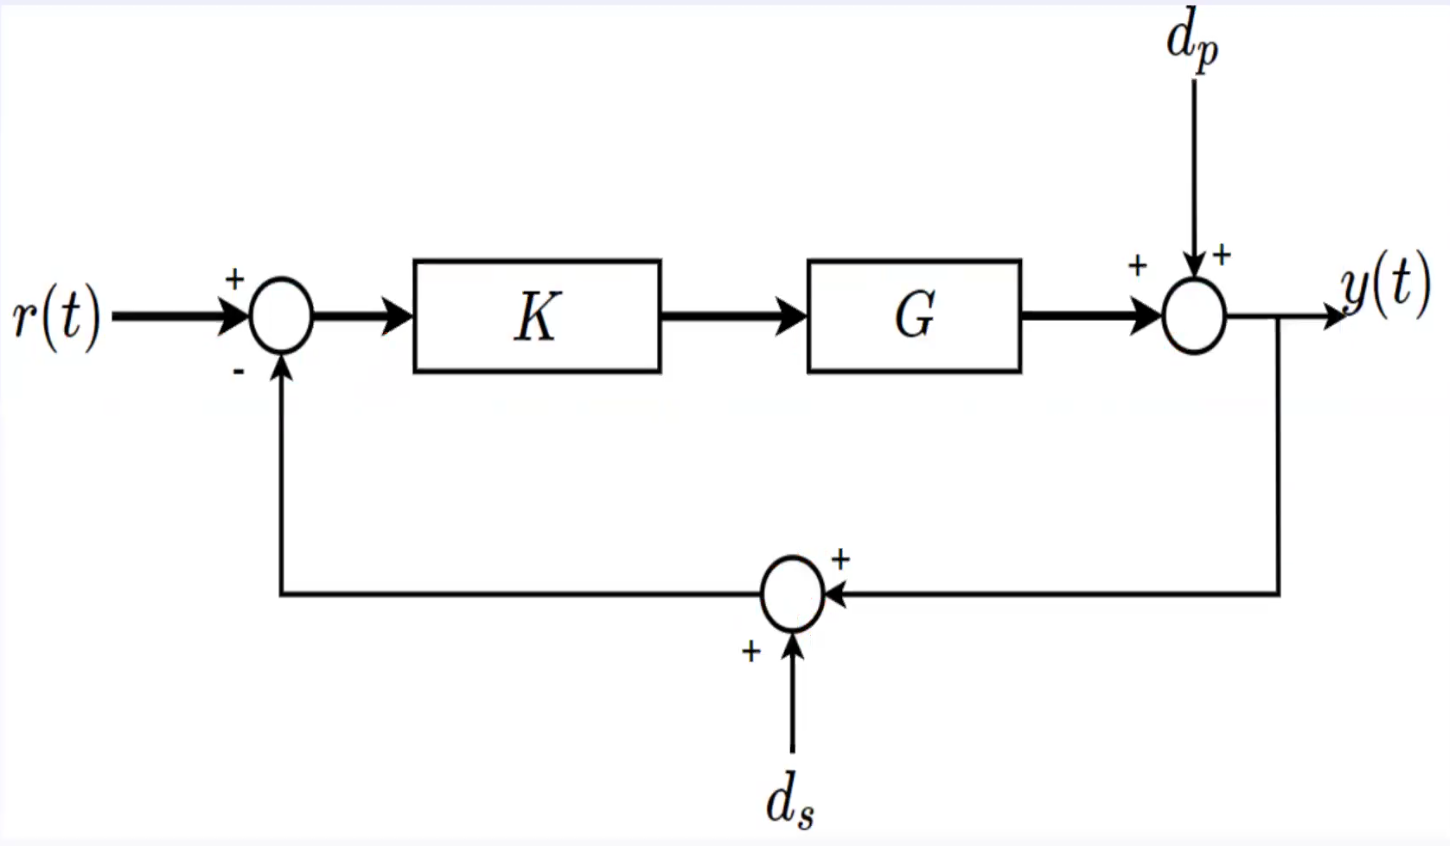
\includegraphics[width=0.6\textwidth]{fic-control-problem.png}
    \caption{The block diagram of the generalized plant used for our ficticious control problem in the $H_\infty$ context}
 \end{figure}
 As a result,
 \[
 M_r(s) = \tilde{T}(s) = \frac{\tilde{K}\tilde{G}}{1 + \tilde{K}\tilde{G}}
 \]
 where
 \[
 \tilde{K} = \arg \min\limits_{\tilde{K}(s) \in \tilde{K}(s)^{stab}} \|T_{wz}(s)\|_\infty
 \]
 and 
 \[
 T_{wz} = 
 \begin{bmatrix}
 W_T\tilde{T}\\
 W_S\tilde{S}
 \end{bmatrix}
 \]
    \end{example}
    \item The true $G$ does have zeros our of the unit circle (non-minimum-phase zeros), we have to include such zeros in the ficticious plant.\\
    If we don't consider them into the plant, while designing the controller, we obtain a $T$, it is possible that we perform an unstable cancellation with the non-minimum phase of the plant. Nonetheless,  it is a problem due to the fact that, in the context of DDDC, it is assumed that we don't know the plant.\\
    In practice, we can start by performing an experiment on $G$ by applying a step input. If the system $G$ has any non-minimum-phase zeros, the step response is going to show an undershoot. \textbf{In this case, we should do something more in order to detect the position of that zero.}
\end{enumerate}



 
 






















\section{Stability Guarantee in Set-Membership Direct Data-Driven Control}

Considering DDDC, if M and the selected controller class are ”appropriate”, a solution exists.
The DDDC procedure leads to a controller built using the central estimate $\rho^c$
\[
K^c \equiv K(q^{-1},\rho^c)
\]

It is possible that the controller that is obtained in this manner, from the SM Identification does not make the closed-loop system stable.

The fact that we have noise in the data makes the problem of determining the stability harder. If we had noise free data, we could estimate perfectly the plant, and checking the stability would have been just checking basic stability criterion for our matrix transfer function.

The noise creates a phenomenon that we obtain an infinite number of models for our plant, so we have to check the stability of all of those systems. For doing so, we have to consider the worst case inside the set.



\subsection{problem setting}

According to the DDDC frmework, stability must be established in the following conditions.
\begin{itemize}
    \item The plant $P$ is known; we assume that the order of the plant is less than or equal to a given integer $n_p$.
    \item The controller $K^c$ has been designed and is fixed.
    \item A set of input-output data $\{r_t,\tilde{y}_t)\}$ collected on the plant is available. The output samples are corrupted by noise according to:
    \[
    \tilde{y}_t = y_t + \eta_t, \hspace{0.5cm} |\eta_t|\leq \Delta_\eta, \hspace{0.5cm} t=1,\,2,\,\cdots,\,N
    \]
\end{itemize}

Uncertainty on the data makes the problem of establishing stability harder. Stability must be ensured for all allowed realizations of the noise within the specified
bound.\\

Intuition: the noise induces uncertainty on the available information.
More uncertainty means harder to achieve stability.

\subsection{$H_\infty$-norm}
$H_\infty$ in the discrete-time domain is defined as follows:
\[
\|G(z)\|_\infty  \sup\limits_{\omega \in [0,\,2\pi]} |G(e^{i\omega})|
\]
\begin{factbox}
Here, we should have an idea about the $H_\infty$, the I studied it in the modern design of control system.\\

The physical intuition about this norm is that, it gives the maximum amplification of the energy of the input that your provide to a system.
\end{factbox}

\subsection{Small-gain theorem}
Almost all the results about the robustness in control theory is based on this theorem. This theory says if two systems $S1$ and $S2$ are connected as the following figure. 

\textbf{Theorem}: Suppose subsystems $S1$ and $S2$ are stable. Then, the interconnection of these two subsystem shown in the figure is \textbf{well-posed} and \textbf{internally stable} if and only if 
\[
\|S_1S_2\|_\infty < 1
\]
It is called in this way because of the previous argument about the energy amplification interpretation of $H_\infty$ norm. 
 \begin{figure}[H]
    \centering
    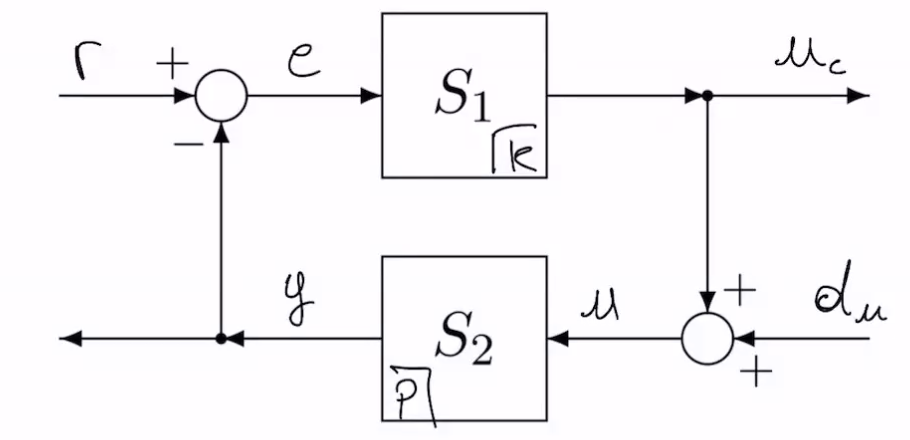
\includegraphics[width=0.4\textwidth]{interconnection-0.png}
    \caption{Inter-connection of two systems; here, S1 is considered as the controller and S2 is considered as the plant to be controlled.}
 \end{figure}


\begin{example}[Example]
Consider an unknown plant $P$. Let $P_n$ be a nominal description of the plant and $W_P$ a description of its uncertainty.\\
Assume that the model belongs to a class of multiplicative uncertainty model as follows:
\[
\{P: P = P_n (1 + W_P \Delta(z)),\,\,\|\Delta\|_\infty <1 \}
\]
Here, $P_n$ and $W_P$ are supposed to be known. \\

Now, we use the small-gain theorem. Considering the feedback control system, we consider $\Delta$ as our subsystem $S1$. 
 \begin{figure}[H]
    \centering
    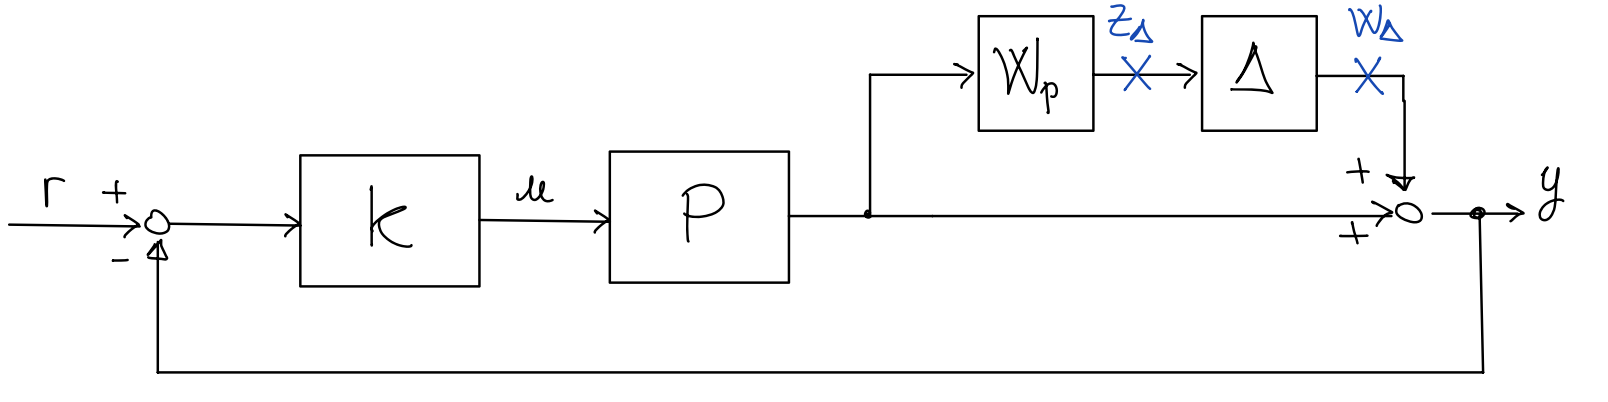
\includegraphics[width=0.75\textwidth]{small-gain-example.png}
    \caption{Block diagram of the feedback control system with uncertainty on the plant; in the discussion of indirect data drive design of controllers.}
 \end{figure}
 \[
 S1 \equiv \Delta \]
 \[
 S2 \equiv G_{w_\Delta z_\Delta} = \frac{-KP_nW_p}{1+KP_n}
 \]
 Here, $S1$ is stable by assumption.  Then, we should study the stability of $S2$. $S2$ is the multiplication of
 \[
 S2 = -T_n*W_p
 \]
 where
 \[
 T_n = \frac{KP_n}{1 + K P_n}
 \]
$W_p$ is stable by assumption, it is a weighting function determining the norm of uncertainty and the uncertainty cannot be infinite for a given frequency. In addition, $T_n$ is stable if $K$ stabilizes the nominal plant.
 
 Small-gain theorem implies that:
 \[
\|S1S2\|_\infty = \|\Delta\frac{-KP_nW_P}{1 + KP_n}\|_\infty < 1
 \]
 and adopting\textbf{ sum-multiplicativity property of induced norms.} 
 \[
 \|\Delta\frac{-KP_nW_P}{1 + KP_n}\|_\infty \leq\|\Delta\|_\infty \|\Delta\frac{KP_n}{1 + KP_n}W_P\|_\infty
 \]
 Since we know that $\|\Delta\|_\infty<1$ we obtain that 
 \[
\|S1S2\|_\infty \leq \|\frac{KP_n}{1 + KP_n}W_P\|_\infty < 1
 \]
 \end{example}
 
\begin{example}
  \begin{factbox}[Induced norm]
 Induced norm is the norm defined by the worst case ratio between two norms in two different space. Since a system is an object which maps signals into signals, we can consider it as an operator between the space of signals. And if we define the norm of a signal as the energy of that signal, $H_\infty$ is the induced norm from the space of bounded energy signals.
 \end{factbox}

which means if 
\[
 \|\frac{KP_n}{1 + KP_n}W_P\|_\infty < 1
\]
the interconnection of the two systems is going to be stable two.
\end{example}


The previous example was about robust stability of a system, and, in general, any attempt to describe the uncertainty around a nominal plant inevitably leads to \textbf{indirect data-driven control}. However, in the connection of DDDC, the plant is unknown.\\

To circumvent this problem, We consider a \textbf{nominal feedback control system} with our \textbf{ideal controller}, and we consider \textbf{the uncertainty} resulting from the noisy data as a \textbf{distance between actual and ideal controller}.\\

 \begin{figure}[H]
    \centering
    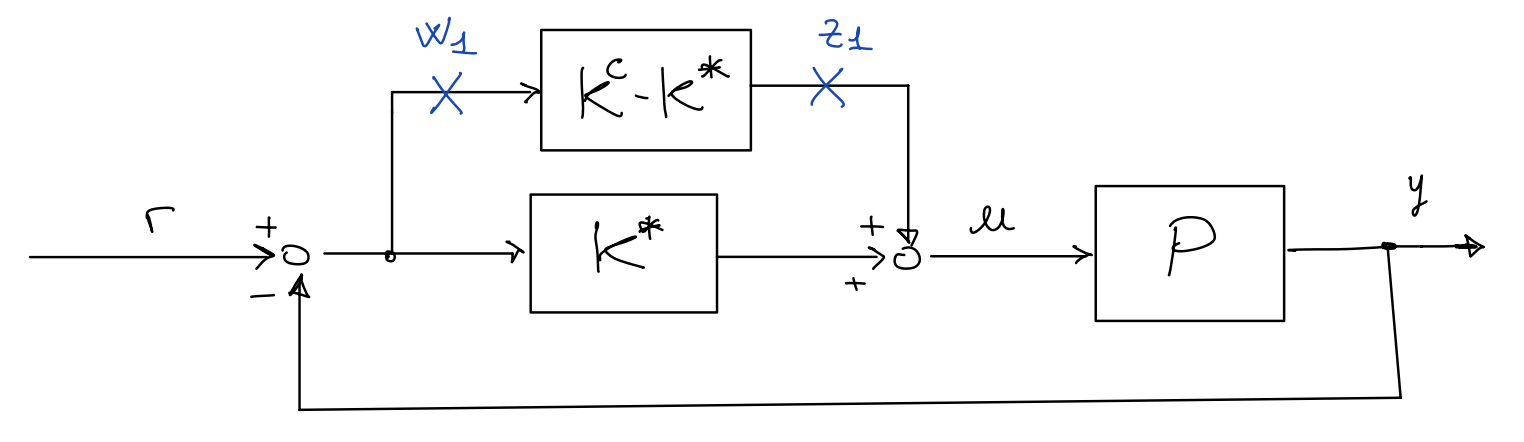
\includegraphics[width=0.75\textwidth]{small-gain-dddc.png}
    \caption{Block diagram of the feedback control system with uncertainty on the controller; this is in the context of DDDC.}
 \end{figure}

As it was discussed, $K^{*}$ is the ideal controller and the uncertainty is the distance of the ideal controller from the central controller $K^{c}$. Therefore,

\[
S1 \equiv K^{c} - K^{*} \:\:\:\: S2 \equiv \frac{-P}{1+K^{*}P} 
\]

Now consider the following theorem:\\
\newpage
\textbf{Small-gain theorem in DDDC}:\\
Let
\[
\Delta(z) = M(z) - K^{c}P(z)(1-M(z))
\]
The controller $K^{c}$ stabilizes the plan $P$ if the following assumptions are satisfied:
\begin{itemize}
    \item The ideal controller $K^{*} = \frac{M}{P(1-M)}$ stabilizes the plant
    \item $\Delta(z)$ is stable
    \item $\|\Delta\|_\infty<1 $
\end{itemize}

So first, we have to show that our subsystems are stable.\\

$S2$ is the transfer function between $u$ and $y$ in the nominal system. Then, $S2$ is stable if the nominal system is stable, which means $K^{*}$ stabilizes the plant, that in turn is \textbf{our first assumption.}\\

Now, $S1$ should be stable. since $S2$ is stable then $S1$ is stable if and only if $S1S2$ is stable.\\


Let us evaluate $S1S2$
\[
S1S2 = (K^{c} - K^{*})\frac{-P}{1+K^{*}P} = \frac{K^{*}P}{1+K^{*}P} - \frac{K^{c}P}{1+K^{*}P} 
\]
It can be notices that the first term is the definition of our ideal sensitivity function and we can pull out an ideal sensitivity function from the second term.
\[
M = T^{*} = \frac{K^{*}P}{1+K^{*}P}
\]
\[
S^{*} = 1 - M = \frac{1}{1+ K^{*}P}
\]
Now, by substituting these two in our equation, the ideal controller is no longer needed to check the stability. By rewriting we obtain:
\[
M - K^{c}P(1-M)
\]
Which is what we considered $\Delta(z)$ in the description of our theorem.

$S1$ is stable if and only if $S1S2$ is stable and if and only if $\Delta$ is stable. \textbf{We consider this as our second assumption.}\\

Finally, 
\[
\|S1S2\|_\infty = \|\Delta\|_\infty < 1
\]
and this is our \textbf{assumption three}.

At this point, it is true that we eleminated $K^{*}$, but still we have the description of the plant in our theorem, which is not known in this context.


Regarding the first assumption, The ideal controller $K^{*} = \frac{M}{P(1-M)}$ stabilizes the plant \textbf{if and only if} $M$ is stable and no unstable cancellations occur, discussed in the previous section.\\
Now, we focus our attention on the second and the third assumption, which is we have to ensure that $\Delta = M - K^{c}P(1-M)$ is stable. To make sure that $\Delta$ is stable we should make sure that its two terms are stable. \textbf{$M$ is stable, since we want the final plant to be stable}. \textbf{$P$ is considered to be stable; otherwise, we would not be able to perform the experiment.} If $K^{c}$ is stable, then this condition is automatically satisfied. So one of the sufficient conditions is that $K^{c}$ is stable.\\

Nevertheless, in practice, stability is not the only requirement. Most often, zero steady-error is also require, and in order to assure that, we require integrators, which make the controller unstable, and we cannot make the reasoning we just made. \\

Then we have our second sufficient condition. That is, $\Delta$ is stable if $M$ and $P$ are stable - the same reasoning as before holds - and if $K^{c}$ is \textbf{unstable only due to poles in} $z = 1$, our \textbf{loop function} $\frac{M}{1-M}$ have the same number of poles in $z = 1$.\\

\textbf{In summary}, in order for the close-loop control system to be internally stable, we need to ensure that $\Delta (z)$ is stable.
Assume $P$ and $M$ are stable. Sufficient conditions for this are:
\begin{itemize}
\item[a)] Kc is stable.
\item[b)] Kc is unstable only due to poles in $z = 1$ and $\frac{M}{1-M}$, or the loop function, have the same number
of poles in $z = 1$.
\end{itemize}

\subsection{How to compute \(\|\Delta(z)\|_\infty\) without using the plant, and given noisy data?}

\begin{enumerate}
\item[$1^{st}$ step:] Consider one frequency at a time. Cast the problem into the SM framework. This is a set-membership \textbf{estimation} problem, \textbf{not an identification} problem, because we do not want to identify a transfer function; instead, we want to obtain a quantity related to a transfer function. We are given the following a-priori information on \(\Delta\):

\begin{itemize}
    \item[I)] Maximum order of the system: Since 
    \[
    \Delta = M - K^cP(1-M),
    \]
    we can say \(\Delta\) is a transfer function in the following form:
    \[
    \Delta(q^{-1}) = \frac{\gamma_0 + \gamma_1 q^{-1} + \cdots + \gamma_{n_\Delta}q^{-n_{\Delta}}}{1 + \delta_1 q^{-1} + \cdots + \delta_{n_\Delta}q^{-n_{\Delta}}}
    \]
    where
    \[
    n_\Delta \leq n_k + n_p + n_M.
    \]
    Here, \(n_k\) is the order of the controller \(K^c\), \(n_p\) is the order of the plant, and \(n_M\) is the order of the reference model \(M\). This relationship comes from the second term of \(\Delta\); note that \(1-M\) always has the same order as \(M\), \(n_M\).

    \item[II)] Definition and plant's data:
    \[
    \Delta(q^{-1})r_t = M(q^{-1})r_t - K^c(q^{-1})(1-M(q^{-1}))P(q^{-1})r_t 
    \]
    Now, we can substitute the following term:
    \[
    P(q^{-1})r_t = y_t = \tilde{y}_t - \eta_t
    \]
    Therefore,
       \[
    \Delta r_t = Mr_t - K^c(1-M)\left[ \tilde{y}_t - \eta_t \right]
    \]
    \[
    \Delta r_t = Mr_t - K^c(1-M)\tilde{y}_t + K^c (1-M)\eta_t
    \]
    here, we call name
    \[
    z_t = Mr_t - K^c(1-M)\tilde{y}_t
    \]
    and
    \[
    F(q^{-1}) = K^c (1-M)
    \]
    
    
\end{itemize}
    \item[$2^{nd}$ step:]  worst-case (max) norm estimation problem.
    
        \[
        \max_{\Delta,\,\eta} |\Delta(e^{i\omega})| \hspace{0.5cm} \text{s.t. } \Delta{q^{-1}}r_t = z_t + F(q^{-1})\eta_t,\,\,\,\,|\eta_t|\leq \Delta_\eta
        \]
        Pay attention that, we are not directly considering the infinity norm, and we are considering the magnitude of a values of the frequency responce for a fixed $\omega$.
        
        
        \item[$3^{rd}$ step:]  recast into polynomial optimization. in order to do so, First $\Delta(e^{i\omega})$ is recated to a polynomial form, and then, the constraint of this optimiztion problem. \\
        First, let $a,\,b \in \mathbb{R}$ be optimmization variables such that
        \[
        \Delta(e^{i\omega}) = a + i b
        \]
        then,
        \[
        |\Delta(e^{i\omega})| = \sqrt{a^2+b^2}\:\: \Longleftrightarrow \:\: \exists t: t=  |\Delta(e^{i\omega})|\hspace{1cm} t^2 = a^2 + b^2
        \]
        Moreover, denote:
        \[
        \begin{bmatrix}
            e^0\\
            e^{i \omega}\\
            e^{2i \omega}\\
            \vdots\\
            e^{in_\Delta \omega}
        \end{bmatrix}
        =
        \begin{bmatrix}
            \rho_0\\
            \rho_1\\
            \rho_2\\
            \vdots\\
            \rho_{n_\Delta}
        \end{bmatrix}
        +
           \begin{bmatrix}
            \sigma_0\\
            \sigma_1\\
            \sigma_2\\
            \vdots\\
            \sigma_{n_\Delta}
        \end{bmatrix}
        \]
As a function of the parameters \(\gamma,\,\delta\), we can evaluate \(\Delta(e^{i\omega})\) as:
\[
\Delta(z) = \frac{\gamma_0 z^{n_\Delta} + \gamma_1 z^{n_\Delta-1} + \cdots + \gamma_{n_\Delta-1} z + \gamma_{n_\Delta}}
{z^{n_\Delta} + \delta_1 z^{n_\Delta-1} + \cdots + \delta_{n_\Delta-1} z + \delta_{n_\Delta}}.
\]
    
    Now, we replace $z$ with $e^{i\omega}$, and for the ease in the notation, we consider $\delta_0 = 1$
    \[
\Delta(e^{i\omega}) = \frac{\gamma_0 e^{i n_\Delta \omega} + \gamma_1 e^{i (n_\Delta-1) \omega} + \cdots + \gamma_{n_\Delta-1} e^{i \omega} + \gamma_{n_\Delta}}
{\delta_0e^{i n_\Delta \omega} + \delta_1 e^{i (n_\Delta-1) \omega} + \cdots + \delta_{n_\Delta-1} e^{i \omega} + \delta_{n_\Delta}} = a + ib
\]
    pay attention that all the terms in $e$ are exactly known and can be considered in the vector form we denoted.

        Then $a,\,b,\,\gamma,\,\delta$ are related by:
\[
\sum_{j=0}^{n_\Delta} \gamma_j e^{i(n_\Delta-j)\omega} 
= 
(a + i b) 
\left[ 
\sum_{j=0}^{n_\Delta} \delta_j e^{i\omega (n_\Delta - j)} 
\right]
\]

here $\delta_0$ is considered to be 1 in order to make the representation more compact. Now, we replace the imaginary parts including $e$ with the cartisian representation of them.
\[
\sum_{j=0}^{n_\Delta} \gamma_j \left( \rho_j + i \sigma_j \right) 
= 
(a + i b) 
\left[ 
\sum_{j=0}^{n_\Delta} \delta_j \left( \rho_j + i \sigma_j \right) 
\right]
\]

\[
\sum_{j=0}^{n_\Delta} \gamma_j \rho_j + i \sum_{j=0}^{n_\Delta} \gamma_j \sigma_j 
= 
\sum_{j=0}^{n_\Delta} a \delta_j \rho_j + i \sum_{j=0}^{n_\Delta} a \delta_j \sigma_j 
+ i b \sum_{j=0}^{n_\Delta} \delta_j \rho_j - b \sum_{j=0}^{n_\Delta} \delta_j \sigma_j
\]

Now we get two equations, the real part on the left-hand side should be equal to the real part on the right-hand side, and the same for the imaginary part.
\[
\sum_{j=0}^{n_\Delta} \gamma_j \rho_j = \sum_{j=0}^{n_\Delta} a \delta_j \rho_j - b \sum_{j=0}^{n_\Delta} \delta_j \sigma_j
\]
For the imaginary part, we obtain:
\[
\sum_{j=0}^{n_\Delta} \gamma_j \sigma_j = + i \sum_{j=0}^{n_\Delta} a \delta_j \sigma_j 
+ i b \sum_{j=0}^{n_\Delta} \delta_j \rho_j
\]

Next, $\delta,\,\gamma$ are related to the data and the noise samples according to:
\[
\Delta(q^{-1})r_t = z_t + F(q^{-1})\eta_t
\]

\[
\frac{\sum_{j = 0}^{n_{\Delta}}\gamma_j q^{-j}}{\sum_{j = 0}^{n_{\Delta}}\delta_j q^{-j}}r_t = z_t + 
\frac{\sum_{j = 0}^{n_F}\beta_j^F q^{-j}}{\sum_{j = 0}^{n_F}\alpha_j^F q^{-j}}\eta_t
\]
where, 
\[
\delta_0 =1
\]
and $\alpha_j^F$ and $\beta_j^F$ are the coefficient of the transfer function $F(q^{-1})$ that we have defined.

\[
\left( \sum_{j=0}^{n_F} \alpha_j^F q^{-j} \right) 
\left( \sum_{j=0}^{n_\Delta} \gamma_j q^{-j} \right) r_t =
\left( \sum_{j=0}^{n_F} \alpha_j^F q^{-j} \right) 
\left( \sum_{j=0}^{n_\Delta} \delta_j q^{-j} \right) z_t +
\left( \sum_{j=0}^{n_F} \beta_j^F q^{-j} \right) 
\left( \sum_{j=0}^{n_\Delta} \delta_j q^{-j} \right) \eta_t
\]

Expanding the products:

\[
\sum_{j=0}^{n_F} \sum_{k=0}^{n_\Delta} \alpha_j^F \gamma_k q^{-(j+k)} =
\sum_{j=0}^{n_F} \sum_{k=0}^{n_\Delta} \alpha_j^F \delta_k q^{-(j+k)} z_t +
\sum_{j=0}^{n_F} \sum_{k=0}^{n_\Delta} \beta_j^F \delta_k q^{-(j+k)} \eta_t
\]

In terms of time-shifted variables:

\[
\sum_{j=0}^{n_F} \sum_{k=0}^{n_\Delta} \alpha_j^F \gamma_k r(t-j-k) =
\sum_{j=0}^{n_F} \sum_{k=0}^{n_\Delta} \alpha_j^F \delta_k z(t-j-k) +
\sum_{j=0}^{n_F} \sum_{k=0}^{n_\Delta} \beta_j^F \delta_k \eta(t-j-k)
\]

Key notes:\\
- $\delta$ other than $\delta_0 = 1$, $\gamma$, $\eta$ are optimization variables here.\\
- \(r(t-j-k)\), \(z(t-j-k)\),  \(\eta(t-j-k)\), $\alpha^F$, $\beta^F$ are fixed values.\\

Overall, the optimization problem is recast to:


\[
\max\limits_{t, a, b \in \mathbb{R}, \, \gamma \in \mathbb{R}^{n_\Delta + 1}, \, \delta \in \mathbb{R}^{n_\Delta}, \, \eta \in \mathbb{R}^N} \quad t
\]
\[
\text{s.t.}
\]
\[
t^2 = a^2 + b^2,
\]
\[
\sum_{j=0}^{n_\Delta} \gamma_j \rho_j = \sum_{j=0}^{n_\Delta} \delta_j \left( a \rho_j - b \sigma_j \right),
\]

\[
\sum_{j=0}^{n_\Delta} \gamma_j \sigma_j = \sum_{j=0}^{n_\Delta} \delta_j \left( a \sigma_j + b \rho_j \right),
\]

\[
\sum_{j=0}^{n_F} \sum_{k=0}^{n_\Delta} \alpha_j^F \gamma_k r(t-j-k) =
\sum_{j=0}^{n_F} \sum_{k=0}^{n_\Delta} \alpha_j^F \delta_k z(t-j-k) +
\sum_{j=0}^{n_F} \sum_{k=0}^{n_\Delta} \beta_j^F \delta_k \eta(t-j-k)
\]

\end{enumerate}

The above problem is a polynomial optimization problem.
Solving it using SDP relaxation, we get an upper bound on the true $\Delta(e^{i\omega})$.\\

Theoretically, the problem must be solved for\textbf{ all frequencies }$\omega \in [0,\,2 \pi]$. \\
Alternatively, we
can introduce a Lipschitz continuity assumption on $|\Delta(e^{i\omega})|$, e.g., assuming that it does
not increase or decay faster than 100 dB/dec or 200 dB/dec.\\

The computed upper bounds on $|\Delta(e^{i\omega})|$ can be made less conservative by increasing
the number of samples used in the formulation of the optimization problem.

\newpage

\begin{example}[example]
    
We perform SM-DDDC from data obtained by simulating the plant:
\[
G(q^{-1}) = \frac{0.09516q^{-1} + 0.02q^{-2} + 0.05q^{-3} - 0.04q^{-4}}{1 - 0.9048q^{-1} + 0.2q^{-2} - 0.5q^{-3} + 0.4q^{-4}}.
\]

The input \( r(t) \) is a random signal with amplitude 1. The output is corrupted by uniform noise in \([-|\epsilon|, +|\epsilon|]\), resulting in a signal-to-noise ratio of 15 dB. The reference model is:
\[
M(q^{-1}) = \frac{0.4q^{-1}}{1 - 0.6q^{-1}}.
\]

The controller order is iteratively searched starting from \( n_K = 1 \). The procedure leads to a feasible optimization problem for \( n_K = 4 \). The central estimate controller to be certified is:
\[
K(\omega_c, z) = \frac{4.176z^4 - 3.68z^3 + 0.7055z^2 - 2.006z + 1.644}{z^4 - 0.7755z^3 + 0.314z^2 - 0.9413z + 0.4028}.
\]

We assume the knowledge of an upper bound on the Lipschitz constant of \( L_b = 200\text{ dB/dec} \).
 \begin{figure}[H]
    \centering
    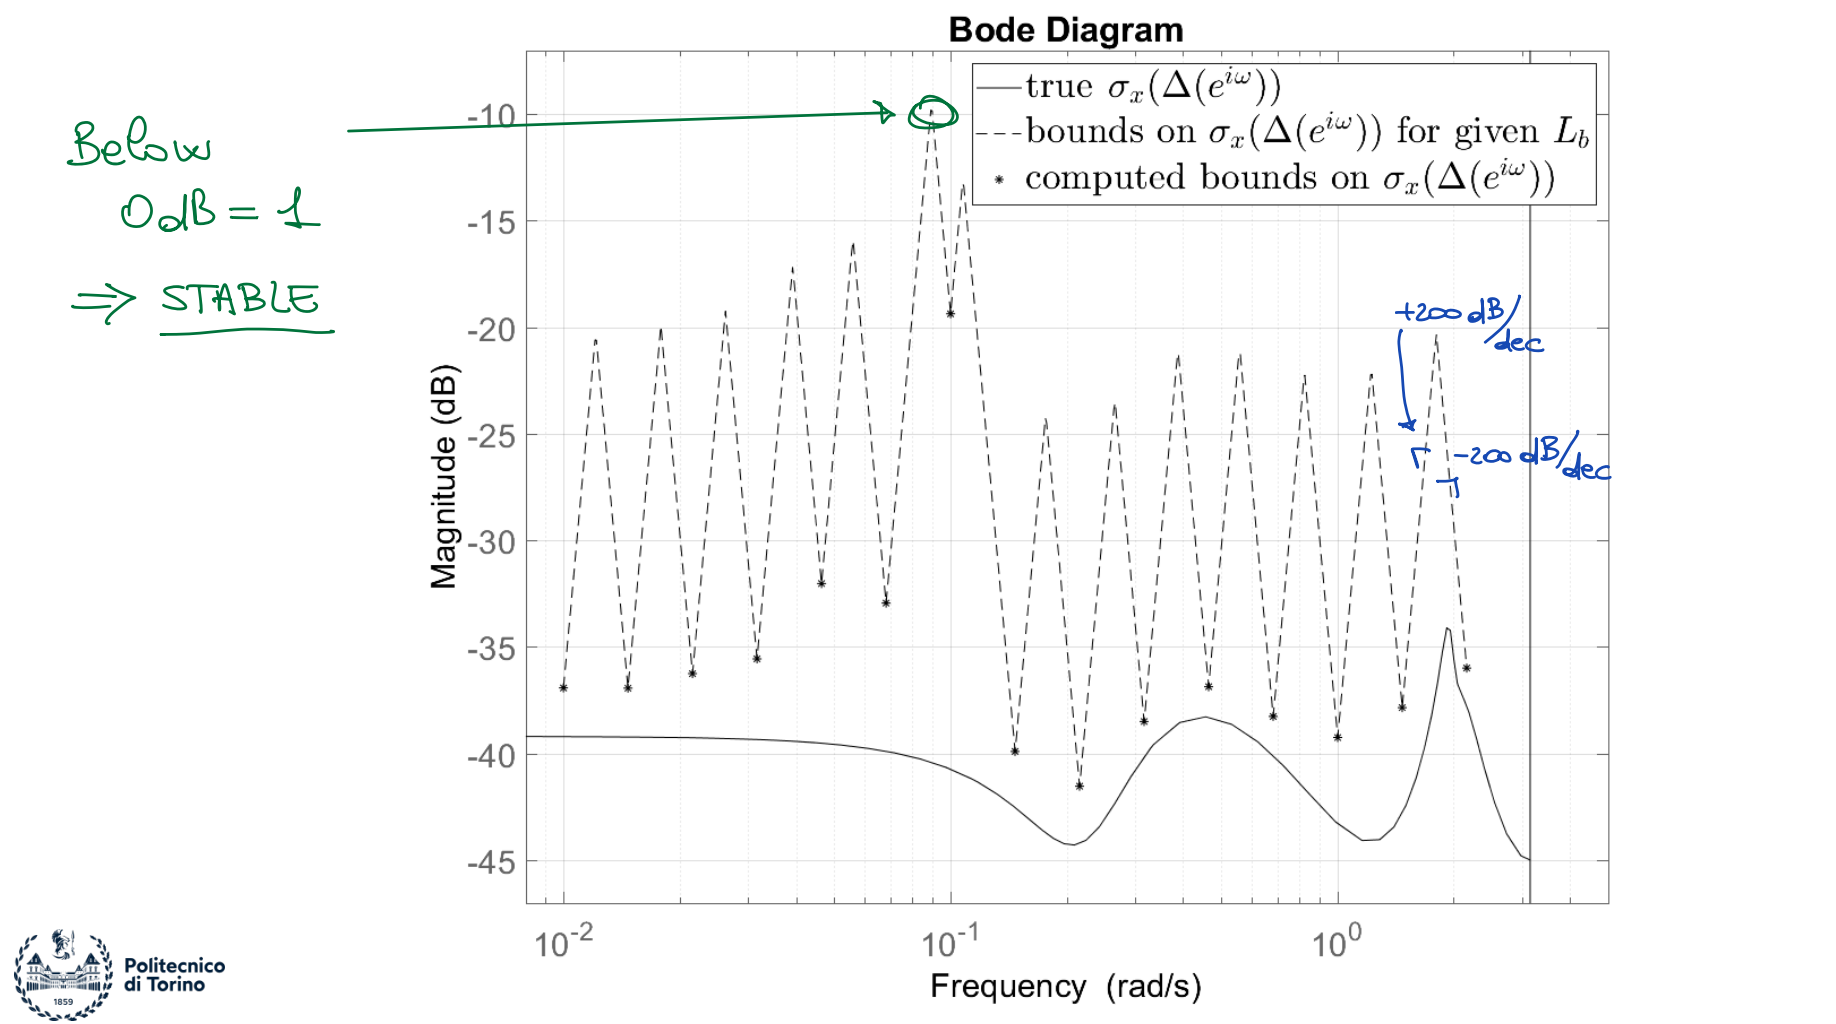
\includegraphics[width=0.75\textwidth]{stability-dddc.png}
    \caption{The solution of the optimization problem for checking the stability of the plant considering the designed controller.}
 \end{figure}
\end{example}
















\chapter{Laboratory 01: solution}

Upon successful completion of this homework, students will
\begin{enumerate}
\item Be able to compute Least Squares (`2 norm) and Least `∞ norm parameter estimation for
Discrete-time LTI systems.
\item Be able to analyze properties and limitations of the considered estimators
\end{enumerate}

The plant to be estimated is a continuous-time LTI dynamical system assumed to be exactly described by the following transfer function:
\[
G_p(s) = \frac {100}{s^2 + 1.2 s + 1}
\]

Assuming the sampling time \(T_s = 1\), the following script is used for discretizing the transfer function of the sysetm, using \textit{zoh}, or zero-order-hold method.

\[G_d = c2d(G_p, Ts, 'zoh')\]

The result going to be of the following form:

\[G_d(z) = \frac{N(z)}{D(z)}\]

The result of this command is as follows:

\[
G_d(z) = \frac{32.24z + 21.41}{z^2 - 0.7647z + 0.3012}
\]

Now, the input of the system is considered to be samples of a uniformly distributed random variable. The command \textit{\(u = rand(N,1)\)} is used at this end. \(N\) is considered to be 1000. Then, the command \textit{ \(y =\)lsim(\(G_d, u, Ts)\)} is used to simulate \textbf{noise-free} output samples. Here, it is assumed that the input of the system is exactly known.


\subsubsection{\(\theta_{LS}\) in ideal noise-free setting}
The regression matrix \(A\) and output vector \(b\), are shaped as follows. It is worthwhile to mention that, in this case, since the samples are noise free, \(N = 7\) suffice to obtain exactly the the values of the parameters.

\[
    y_{Noise Free} = A_{Noise Free}\theta
\]
where \(y = [y(3) y(4) ... y(N)]^T, \theta = [\theta_1 \theta_2 ... \theta_5]^T)\), and
\[
    A = \left[
    \begin{matrix}
    -y(2) & -y(3) & u(3) & u(2) & u(1) \\
    -y(3) & -y(2) & u(4) & u(3) & u(2) \\
    \cdots & \cdots & \cdots & \cdots & \cdots   \\
    \cdots & \cdots & \cdots & \cdots & \cdots   \\
    -y(N-1) & -y(N-2) & u(N) & u(N-1) & u(N-2)
    \end{matrix} 
    \right]\\
\]
The command used for deriving \(\theta's\) is:
\[
\theta_{LS} = y \ A
\]

It can be seen that the parameters obtained in this way are exactly parameters of the discretized transferfunction, except for arithmatic roundings.
\[
\begin{bmatrix}
    \theta_{LS} & \theta_{Gd} \\
    -0.7647 & -0.7647 \\
     0.3012 & 0.3012 \\
    -0.0000 & 0 \\
    32.2369 & 32.2369 \\
    21.4103 & 21.4103
\end{bmatrix}
\]

\subsubsection{\(\theta_{LS}\) in Equation-Error setting}
In the second part, it is asked to repeat the process of estimation, simulating an error that affect the equation. In this case the collected measurement y are give by:
\[
D_d(q^{-1})y_t = N_d(q^{-1})u_t + e_t
\]
\begin{QandAbox}
This assumption about the noise structure is theoretical, and it is not according to read data acquisition setting, which is Error-in-Variable setting or, assuming input to be exactly known Output-Error setting
\end{QandAbox}
Here, the error, \(e\), is considered to be a normaly distributed noise with standard deviation 5.
\[
e = 5 * randn(N,1)
\]

To create output data samples that is affected in this manner, the noise entering each output sample should be filtered by \(D(z)\)the denuminator of \(G_d\). Therefore the following MATLAB code should be used:
\[
\text{[num, den]} = tfdata(Gd, 'v')
y\_EE = lsim(Gd,u) + lsim(tf(1,den),e)
\]

In this case, the regression matrix is shaped by the noisy output samples. Hence:
\(y_{EE} = [y_{EE}(3) \: y_{EE}(4) ... y_{EE}(N)]^T 
\)
\[
    A = \left[
    \begin{matrix}
    -y_{EE}(2) & -y_{EE}(3) & u(3) & u(2) & u(1) \\
    -y_{EE}(3) & -y_{EE}(2) & u(4) & u(3) & u(2) \\
    \cdots & \cdots & \cdots & \cdots & \cdots   \\
    \cdots & \cdots & \cdots & \cdots & \cdots   \\
    -y_{EE}(N-1) & -y_{EE}(N-2) & u(N) & u(N-1) & u(N-2)
    \end{matrix} 
    \right]\\
\]

The result of the Least square algorithm is going to be as follow:
\[
\begin{bmatrix}
    \theta_{EE} & \theta_{Gd} \\
    -0.7762 & -0.7647 \\
     0.3116 & 0.3012 \\
     0.2078 & 0 \\
    32.2405 & 32.2369 \\
    21.0843 & 21.4103
\end{bmatrix}
\]
As it can be seen, the result is very close to the observed values. Since this structure of the noise satisfies both assumptions of the consistency property of Least Squares, it is guaranteed that as \(N\) tends to infinity, the values of \(\theta\) will converge to the true values, regardless of how large the standard deviation of the noise affecting

\subsubsection{\(\theta_{LS}\) in Output-Error setting}
The noise in this setting directly affect the output measurements
\[
y_t = G_d(q^{-1})u_t + \eta_t
\]
\begin{QandAbox}
This setting is a good structure compliant with the real data acquisition setting.
\end{QandAbox}
Here, the error, \(\eta_t\), is considered to be a normaly distributed noise with standard deviation 5.
\[
eta = 5 * randn(N,1)
\]

To create output data samples that is affected in this manner, the following MATLAB code should be used:
\[
y\_OE = lsim(Gd,u) + eta
\]

In this case, the regression matrix is shaped by the noisy output samples. Hence:
\(y_{OE} = [y_{OE}(3) \: y_{OE}(4) ... y_{OE}(N)]^T 
\)
\[
    A = \left[
    \begin{matrix}
    -y_{OE}(2) & -y_{OE}(3) & u(3) & u(2) & u(1) \\
    -y_{OE}(3) & -y_{OE}(2) & u(4) & u(3) & u(2) \\
    \cdots & \cdots & \cdots & \cdots & \cdots   \\
    \cdots & \cdots & \cdots & \cdots & \cdots   \\
    -y_{OE}(N-1) & -y_{OE}(N-2) & u(N) & u(N-1) & u(N-2)
    \end{matrix} 
    \right]\\
\]

The result of the Least square algorithm is going to be as follow:
\[
\begin{bmatrix}
    \theta_{OE} & \theta_{Gd} \\
    -0.5369 & -0.7647 \\
     0.1352 & 0.3012 \\
    -0.2887 & 0 \\
    32.0653 & 32.2369 \\
    28.1921 & 21.4103
\end{bmatrix}
\]
Since this noise structure does not satisfy the second assumption of the consistency property of the least square method, no matter how large \(N\) is, the estimation values are not going to converge to the real values.


\chapter{Laboratory 02: solution}
\section{the first problem}
In this problem we assume that the plant to be identified is exactly described as a discrete-time
LTI models described by the following transfer function (in the \(q^{-1}\) operator):
\[
G_p(q^{-1}) = \frac {\theta_2}{1 + \theta_1q^{-1}}
\]
where
\[
\theta = \left[-0.5 2 \right]
\]
Now, it is required to compute a set-membership estimation of the parameters of the system by means of the following procedure:\\
Assume that the uncertainty affecting the input output data enters the problem according to an equation error structure. Furthermore, to perform the simulation, assume that collected input sequence \(\tilde{u}\) and the unknwon equation error sequences e are as follows :
\[
\tilde{u} = \left[4,\,-3,\,2,\, 1 \right]^T
\]
and
\[
e = \left[0.05,\,-0.25,\,0.3,\,-0.5 \right]^T
\]
Perform a simulation of model in order to collect the input and output data to be used for identification. The output sequence \(tilde{y}\) has to be computed according to the following equation (equation error structure):\\
Based on the transfer function at hand the difference equation of the system is as follow:
\[
y(k) = -\theta_1y(k-1) + \theta_2u(k)
\]
Considering an \textit{Equation-Error} structure for the noise, the following relationship is obtained:
\[
\tilde{y}(k) = -\theta_1 \tilde{y}(k-1) + \theta_2u(k) + e(k)
\]
Where it is assumed that the error \(e\) is known to be bounded as \(|e(k)|\leq \Delta e\) and assuming as initial condition \(\tilde{y}\).

Considering the difference equation of the system, the following information can be obtained:\\
\begin{itemize}
\item \(n_a = 1\) which represent the order of the system, which corresponds to the number of previous samples of \(y\) needed to express the difference equation of the system.
\item \(n_b\) the number of input samples in the difference equation.
\item \(t_{min} = \max(\left[n_a +1, n_b\right]\)
\end{itemize}
MATLAB code for simulation of the system is as follows. Take into account that, alternatively, we could use:
\[
\tilde{y} = \text{lsim}(G_p,u) + \text{lsim}(\text{tf}(1,D,1),e);
\]

\begin{example}
\begin{lstlisting}[caption=Set-membership estimation with theta bounds and simulation]
close all
clear variables
clc
format compact

%% Defining system
z = tf('z',1);
theta = [-0.5 2];
Gp = theta(2)/(1 + theta(1)*z)

u_tilde = [4 -3 2 1]';
e = [0.05 -0.25 0.3 -0.5]';

%% Simulation
% y_tilde(k) = -theta_1*y_tilde(k-1) + theta_2 u_tilde(k) + e(k)
na = 1; % The number of state variables or last samples of y
nb = 1; % The number of past inputs
N = 4;
t_min = max([na+1 , nb]);
y_tilde = zeros(4,1); 
% Initial value

for k = t_min:N
    y_tilde(k) = -theta(1)*y_tilde(k-1) + theta(2)*u_tilde(k) + e(k);
end

%% Upper and lower bound
delta_e = 0.5;
y_up = y_tilde + delta_e;
y_low = y_tilde - delta_e;
plot(1:N, [y_up, y_tilde, y_low])
\end{lstlisting}
\end{example}

In order to obtain \textit{Feasible Uncertainty Set}, it is required to do the following manipulations, considering the definition of FPS we have:
\[
\mathbb{D}_\theta = \left\{ \theta | \tilde{y}(k) + \theta_1 \tilde{y}(k-1) + \theta_2\tilde{u}(k)| \leq \Delta e \forall k \right\}  
\]
Writing exampding the equations for \(t_{min}\) to \(N = 4\), which is the number of samples, we obtain:
\begin{align*}
|\tilde{y}(2) + \theta_1 \tilde{y}(1) + \theta_2\tilde{u}(2)| &\leq \Delta e \\
|\tilde{y}(3) + \theta_1 \tilde{y}(2) + \theta_2\tilde{u}(3)| &\leq \Delta e \\
|\tilde{y}(4) + \theta_1 \tilde{y}(3) + \theta_2\tilde{u}(4)| &\leq \Delta e
\end{align*}
and therefore,
\begin{align*}
-\Delta e - \tilde{y}(2) \geq \theta_1 \tilde{y}(1) + \theta_2\tilde{u}(2) &\leq \Delta e - \tilde{y}(2) \\
-\Delta e - \tilde{y}(3) \geq \theta_1 \tilde{y}(2) + \theta_2\tilde{u}(3) &\leq \Delta e - \tilde{y}(3) \\-\Delta e - \tilde{y}(4) \geq \theta_1 \tilde{y}(3) + \theta_2\tilde{u}(4) &\leq \Delta e - \tilde{y}(4) 
\end{align*}

In each of these relationships, each inequality is a constraint in parameter space that needs to be satisfied so that the equation error becomes less that \(\Delta e\). For finding \(\mathbb{D}_\theta\) in the parameter space, we can consider inequalities as equality, and by doing so, we obtain the equation of 3 pairs of parallel lines on the parameter space, which in this case is a two-dimensional plane. After writing the following MATLAB code, the intersections of all the regiones between the top bound and lower bounds lead to FPS. The plot of the feasible uncertaintly set in the parameter space is as follows:
\begin{example}
\begin{lstlisting}
%% Theta_1 variation
theta_1 = linspace(-5, 5, 1000);
figure,
hold on
for k = t_min:N
    theta_2_up = (+delta_e + y_tilde(k) + theta_1*y_tilde(k-1)) / u_tilde(k);
    theta_2_low = (-delta_e + y_tilde(k) + theta_1*y_tilde(k-1)) / u_tilde(k);
    plot(theta_1, theta_2_low, 'b')
    plot(theta_1, theta_2_up, 'r')
end

%% Brute-force approach (not recommended)
figure,
hold on
for theta_1 = -100:0.01:100
    for theta_2 = -100:0.01:100
        for k = t_min:N
            f = 1; % Flag
            if(abs(y_tilde(k) + theta_1*y_tilde(k-1) - theta_2*u_tilde(k)) > delta_e)
                f = 0;
                break
            end
        end
        if (f == 1)
            plot(theta_1, theta_2, '+');
        end
    end
end
\end{lstlisting}
\end{example}


\begin{figure}[htbp]  % "h" for here, "t" for top, "b" for bottom, "p" for float page
    \centering
    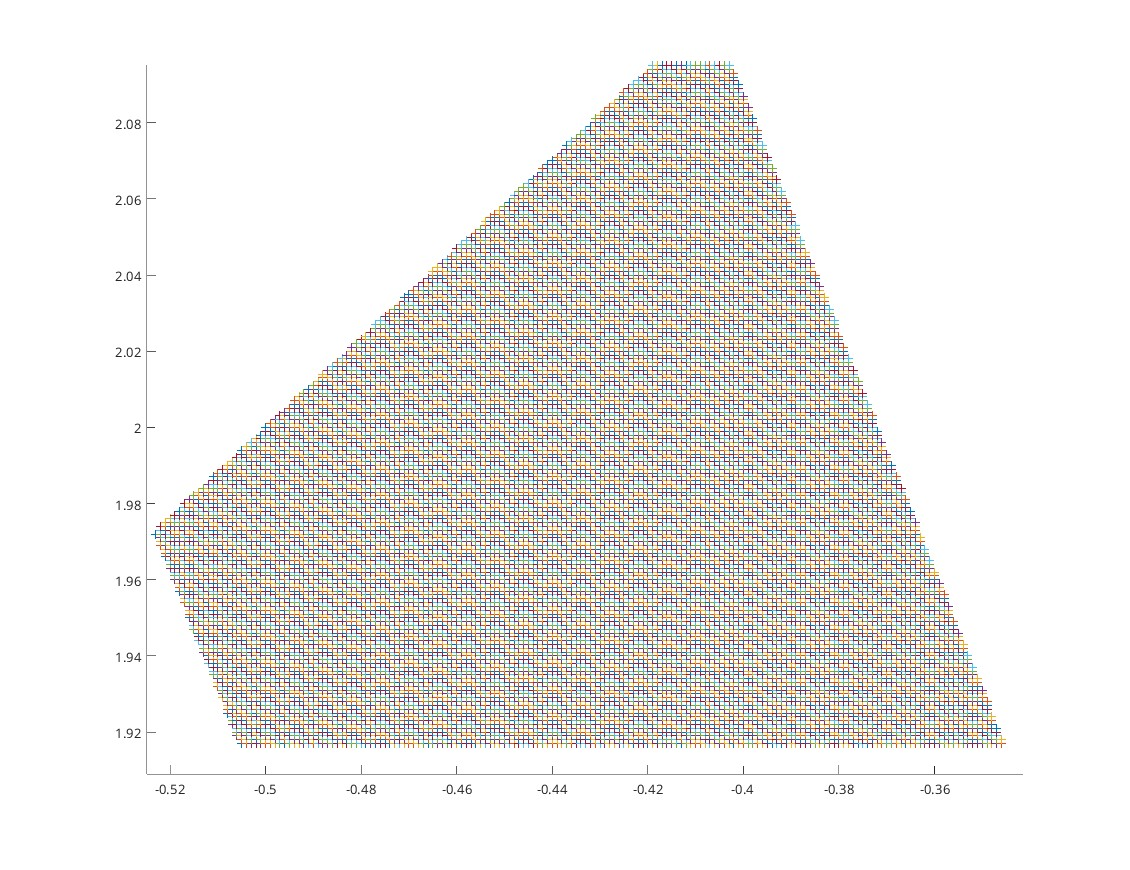
\includegraphics[width=0.65\textwidth]{images/FPS.jpg}
    \caption{FPS represented in the parameter space; the horizontal axis is \(\theta_1\) and the vertical axis is \(\theta_2 \)}
    \label{fig:PFS}
\end{figure}

It can be seen that the "real value" of the parameters is one of point at the top left corner of the \(\mathbb{D}_\theta\).

\section{The second problem}
In this problem we assume that the plant to be identified is exactly described as a discrete-time
LTI models described by the following transfer function:
\[
G_p(q^{-1}) = \frac{N(q^{-1})}{D(q^{-1})} = \frac{\theta_3 + \theta_4 q^{-1} + \theta_5 q^{-2}}{1 + \theta_1 q^{-1} + \theta_2 q^{-2}} \tag{5}
\]
where:
\[
\theta = [\theta_1, \theta_2, \theta_3, \theta_4, \theta_5] = [-0.7647, 0.3012, 0, 32.24, 21.41]
\]


Assuming that the uncertainty affecting the input-output data enters the problem according to an equation error structure, the following simulation is to be performed. The input sequence \( u(t) \) is a random sequence uniformly distributed in \([0, 1]\), and the output sequence \( y(t) \) is computed using the following equation:

\[
    y(t) = -\theta_1 y(t-1) - \theta_2 y(t-2) + \theta_3 u(t) + \theta_4 u(t-1) + \theta_5 u(t-2) + e(t) \tag{7}
\]

where \( \theta = [\theta_1, \theta_2, \theta_3, \theta_4, \theta_5] \) are the model parameters, and \( e(t) \) is a random sequence uniformly distributed in \([- \Delta e, \Delta e]\). The goal is to collect input and output data to be used for identification purposes.

The simulation setup includes:
\begin{itemize}
    \item A random input sequence \( u(t) \), uniformly distributed in \([0, 1]\).
    \item A random error sequence \( e(t) \), uniformly distributed in \([- \Delta e, \Delta e]\).
    \item Output \( y(t) \) calculated according to the equation error model.
\end{itemize}


\begin{example}
\begin{lstlisting}[caption=Set-membership estimation with theta bounds and simulation]
clear variables
close all
format compact
rng('default')
%% defining the system
%LTI 2nd order, a-priori info
theta = [-0.7647,0.3012,0,32.24,21.41];

num = [theta(3) theta(4) theta(5)]
den = [1 theta(1) theta(2)];

Gp = tf(num,den,-1);

%% Simulation
N = 1000;
na = 2;
nb = 3;
tmin = max([na+1,nb]);

y = zeros(N,1);
u = rand(N,1);
delta_e = 0.5; %consider 0.1, 1, 10, 100
for t = tmin:N
    e = 2*delta_e*rand -delta_e; %uniform between[-delta_e,delta e]
    y(t) = -theta(1)*y(t-1) -theta(2)*y(t-2) + theta(3)*u(t) + theta(4)*u(t-1)+...
        theta(5)*u(t-2)+ e;
end
\end{lstlisting}
\end{example}

The relation for feasible parametric set is as follows:
\[
\mathbb{D}_\theta = \{\theta \in \mathbb{R}^5: \tilde{y}-e \leq y \leq \tilde{y}+e \:\text{ s.th.   } |e(.)|\leq \Delta_e\} 
\]

Then, we can formulalte a linprog problem that can be solved as follows:
\begin{example}
\begin{lstlisting}[caption=Set-membership estimation with theta bounds and simulation]
%the rest of the code
%% PUI problem solving by linprog
F = eye(5);
A1 = [-y(tmin-1:N-1), -y(tmin-2:N-2) u(tmin:N) u(tmin-1:N-1) u(tmin-2:N-2)];
A =[A1;-A1]; %for linprog
b1 = y(tmin:N) + delta_e;
b2 = -y(tmin:N) + delta_e;
b = [b1;b2];

% options = optimoptions('linprog', 'ScaleProblem', 'obj-and-constr', 'Display', 'none');
% x = linprog(sign * F(i,:)', A, b, [], [], [], [], options);

PUI = zeros(5,2);
sign = -1; %initialization

for j = 1:2
    sign = -1*sign;
    for i = 1:5
        PUI(i,j) = F(i,:)*linprog(sign*F(i,:)',A,b);
    end
end

PUI

\end{lstlisting}
\end{example}


\chapter{Laboratory 02b: solution}
\begin{QandAbox}
In order to solve this problem, \textit{SparsePOP} and \textit{Sedumi}, toolboxes should be installed, there exist one tutorial file.
\end{QandAbox}
consider the following problem:
\[
\begin{array}{c}
x^* = \arg\,\min\limits_{x} x_1^2 + x_2^2 - 4x_1 - 6x_2 + 13\\
\text{ s.t. }\\[1em]
x_1x_2 - 7x_2 = 10\\ [1em]
x_2 \geq -\frac{1}{2}x_1 +1
\end{array}
\]
The cost function here is a polynomial, which is a sum of \textit{monomial} terms. Each monomial is of the following form:
\[
\alpha x_1^{C_1} x_2^{C_2} \cdots x_n^{C_n}
\]

\begin{example}[Drawing the contour]
\begin{lstlisting}
clear; close all; clc;

%% Part 1: plot
x1_lw = -15; x1_up = +15;
x2_lw = -12; x2_up = +12;

x1 = linspace(x1_lw, x1_up);
x2 = linspace(x2_lw, x2_up);
% objective function
[X1,X2] = meshgrid(x1,x2);
Z = X1.^2 + X2.^2 - 4.*X1 - 6.*X2 + 13;
figure, contour(X1,X2,Z,5*(1:50)');

% equality constraint
x2_1 = linspace(0.01, x2_up);
x2_2 = linspace(x2_lw, -0.01);
x1_1 = (10+7.*x2_1)./x2_1;
x1_2 = (10+7.*x2_2)./x2_2;
hold on; plot(x1_1,x2_1, 'k',x1_2,x2_2, 'k');
axis([x1_lw,x1_up,x2_lw,x2_up]);
\end{lstlisting}
\end{example}


\begin{example}
\begin{lstlisting}
% inequality constraint
x2_ineq = -0.5*x1 + 1;
hold on; plot(x1, x2_ineq, 'b');
patch([x1(1); x1(end); x1_up; x1_lw], ...
    [x2_ineq(1); x2_ineq(end); x2_up; x2_up], ...
    'blue', 'FaceColor', 'blue', 'FaceAlpha', 0.1);
\end{lstlisting}
\end{example}
The resultant graph is as follows:

\begin{figure}[htbp]  % "h" for here, "t" for top, "b" for bottom, "p" for float page
    \centering
    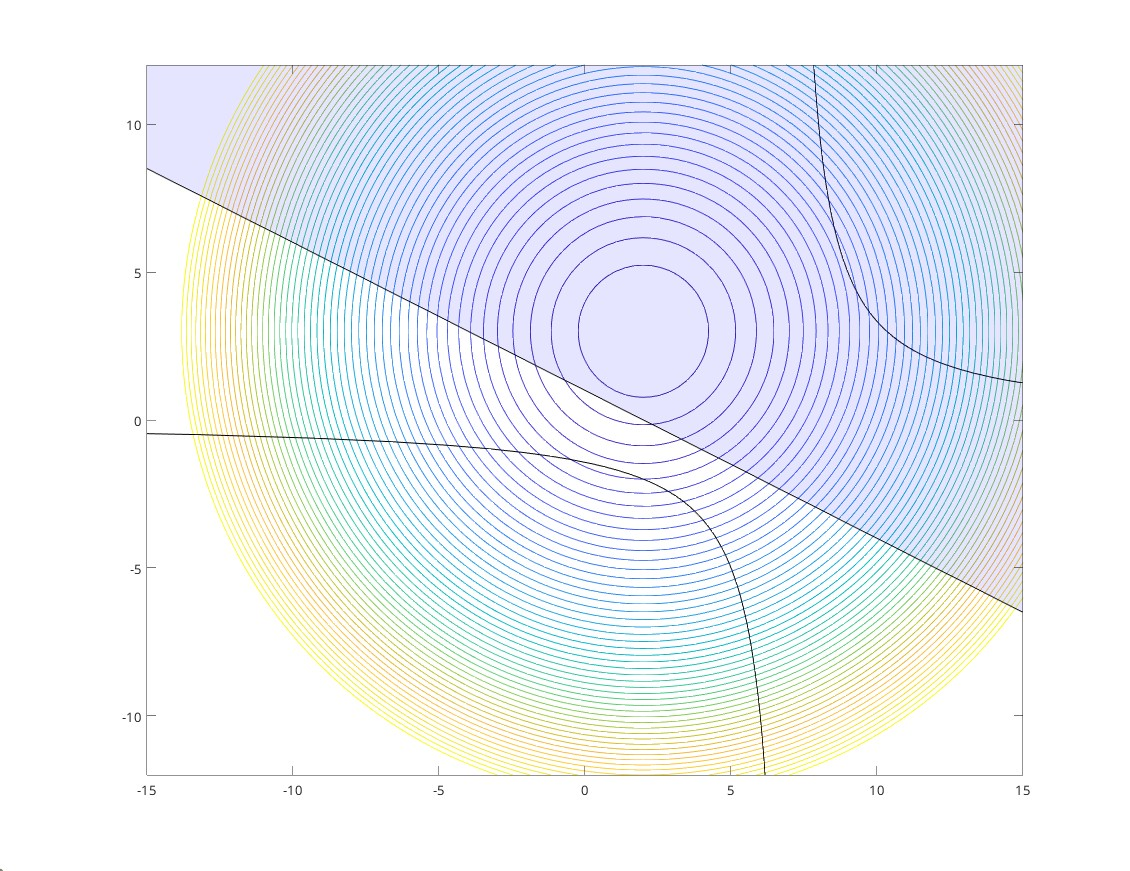
\includegraphics[width=0.75\textwidth]{images/lab02_contour.jpg}
    \caption{The contour of the polynomial as well as the graph of the constraints}
    \label{fig:constraints}
\end{figure}

Let's create the polynomial to be minized, named \textbf{objPoly}:

\begin{example}[Definig the polynomila to be optimized]
\begin{lstlisting}
% objective function
objPoly.noTerms = 5;
objPoly.dimVar = 2;
objPoly.typeCone = 1;  %always to be set to 1
objPoly.degree = 2; %the degree of the poly
objPoly.supports = [2 0; 0 2; 1 0; 0 1; 0 0];
objPoly.coef = [1, 1, -4, -6, 13]'; %should be a column vector
\end{lstlisting}
\end{example}
Pay attention that the support matrix should be made according to the following scheme:

\begin{figure}[ht]  % "h" for here, "t" for top, "b" for bottom, "p" for float page
    \centering
    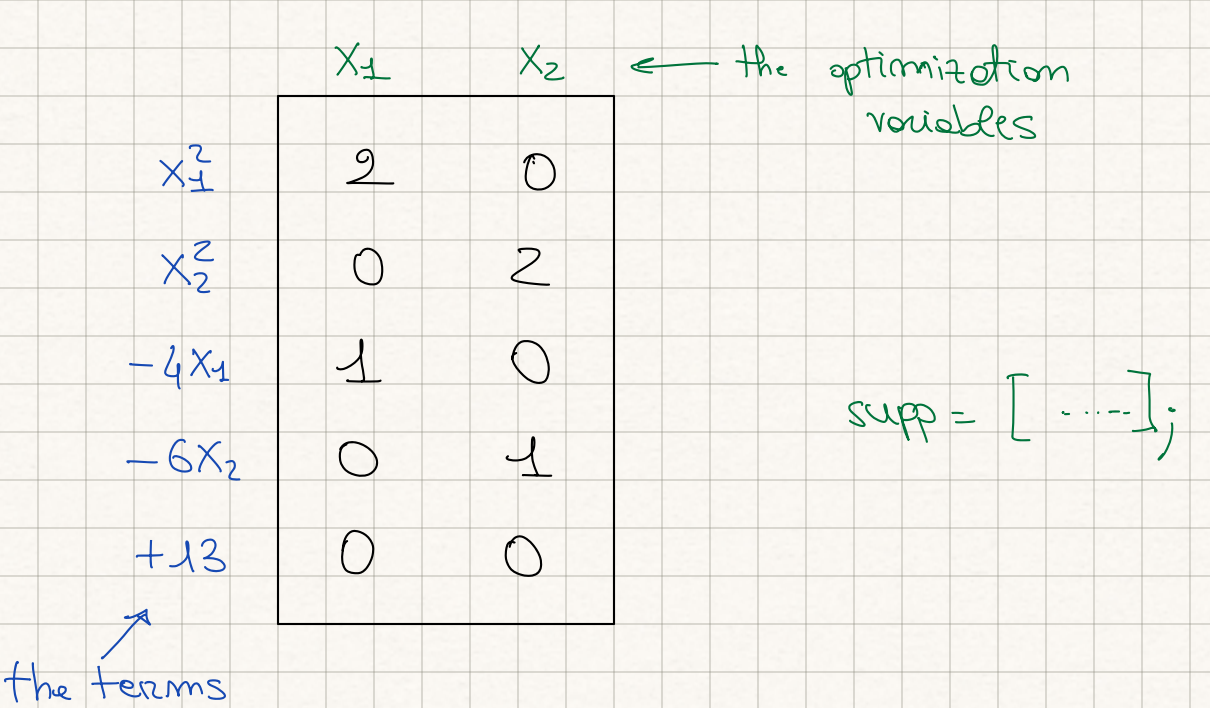
\includegraphics[width=0.75\textwidth]{images/support-matrix.png}
    \caption{The contour of the polynomial as well as the graph of the constraints}
    \label{fig:constraints}
\end{figure}

The inequality and equality constraints should be defined as cell array structures. Pay attention that:
\begin{itemize}
\item \textbf{Equality}: .typeCone = -1
\item \textbf{Inequality}: .typeCone = 1
\end{itemize}

\begin{example}[Definig the polynomila to be optimized]
\begin{lstlisting}
% equality constraint
c = 1;
ineqPolySys{c}.noTerms = 3;
ineqPolySys{c}.dimVar = 2;
ineqPolySys{c}.typeCone = -1; % equality
ineqPolySys{c}.degree = 2;
ineqPolySys{c}.supports = [1 1; 0 1; 0 0];
ineqPolySys{c}.coef = [1 -7 -10]';
% inequality constraint
c = 2;
ineqPolySys{c}.noTerms = 3;
ineqPolySys{c}.dimVar = 2;
ineqPolySys{c}.typeCone = +1; % inequality
ineqPolySys{c}.degree = 1;
ineqPolySys{c}.supports = [0 1; 1 0; 0 0];
ineqPolySys{c}.coef = [1 0.5 -1]';
\end{lstlisting}
\end{example}

After defining the lower bounds and upper bounds for the optimization variables, the \textbf{relaxation order} should be chosen. For this lab, it is recommended that one tries with relaxation orders 1, 2, 3, 4 to solve the problem.

\begin{example}[Solving the optimization problem]
\begin{lstlisting}
% lower bound
lbd = -1e10*ones(2,1);
% upper bound
ubd = +1e10*ones(2,1);

param.relaxOrder = 3;
param.POPsolver = 'interior-point';

[a,b,POP] = sparsePOP(objPoly, ineqPolySys, lbd, ubd, param);
sol_relaxed = POP.xVect;
sol_refined = POP.xVectL;

hold on; 
plot(sol_relaxed(1),sol_relaxed(2),'r*');
plot(sol_refined(1),sol_refined(2),'m*');
\end{lstlisting}
\end{example}

For relaxation order 1 and 2, it can be seen that the solution of the optimization problem does not respect the constraints. That is, the solution is not acceptable.

\begin{figure}[htbp]  % "h" for here, "t" for top, "b" for bottom, "p" for float page
    \centering
    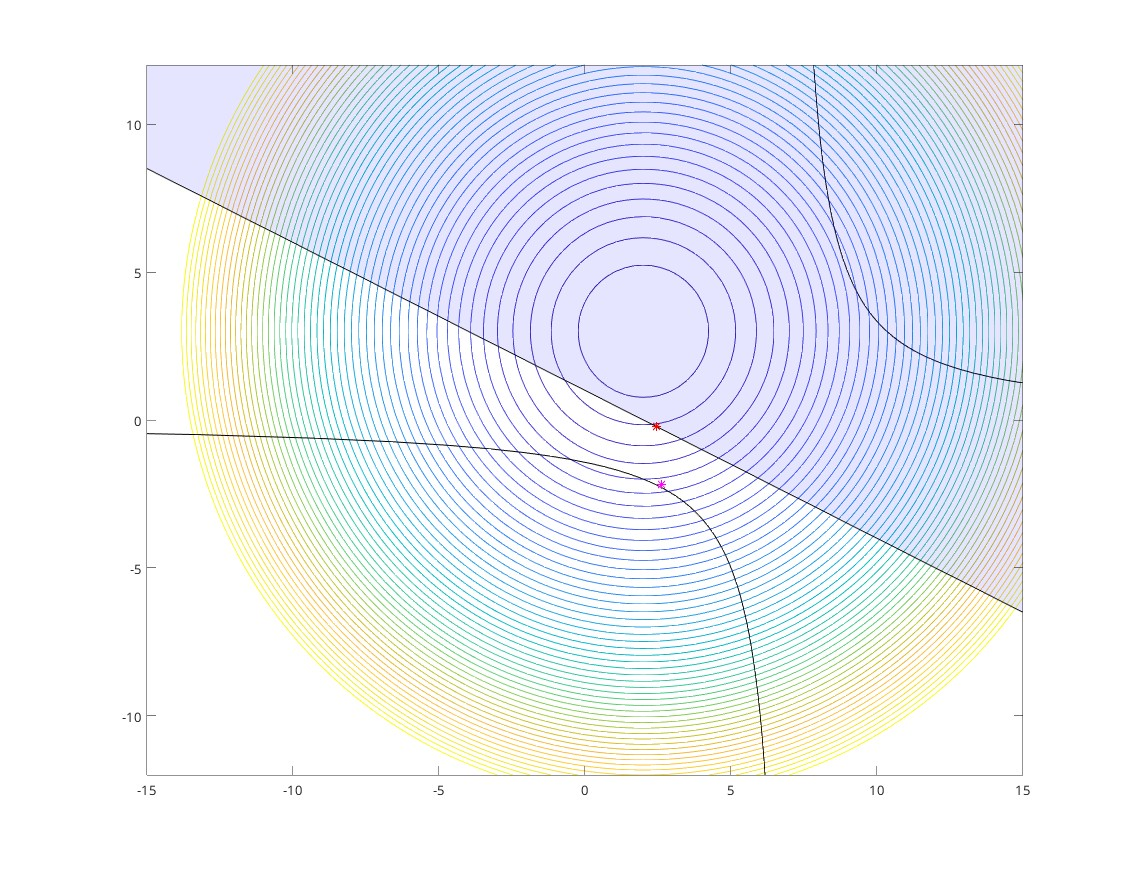
\includegraphics[width=0.75\textwidth]{images/relaxed1.jpg}
    \caption{The solution of the problem with relaxation order 1, the red star spots the relaxed solution and the other star the refined solution, which is the result of sedumi}
    \label{fig:constraints}
\end{figure}

With the relaxation order 3, the problem has an acceptable solution.


\begin{figure}[htbp]  % "h" for here, "t" for top, "b" for bottom, "p" for float page
    \centering
    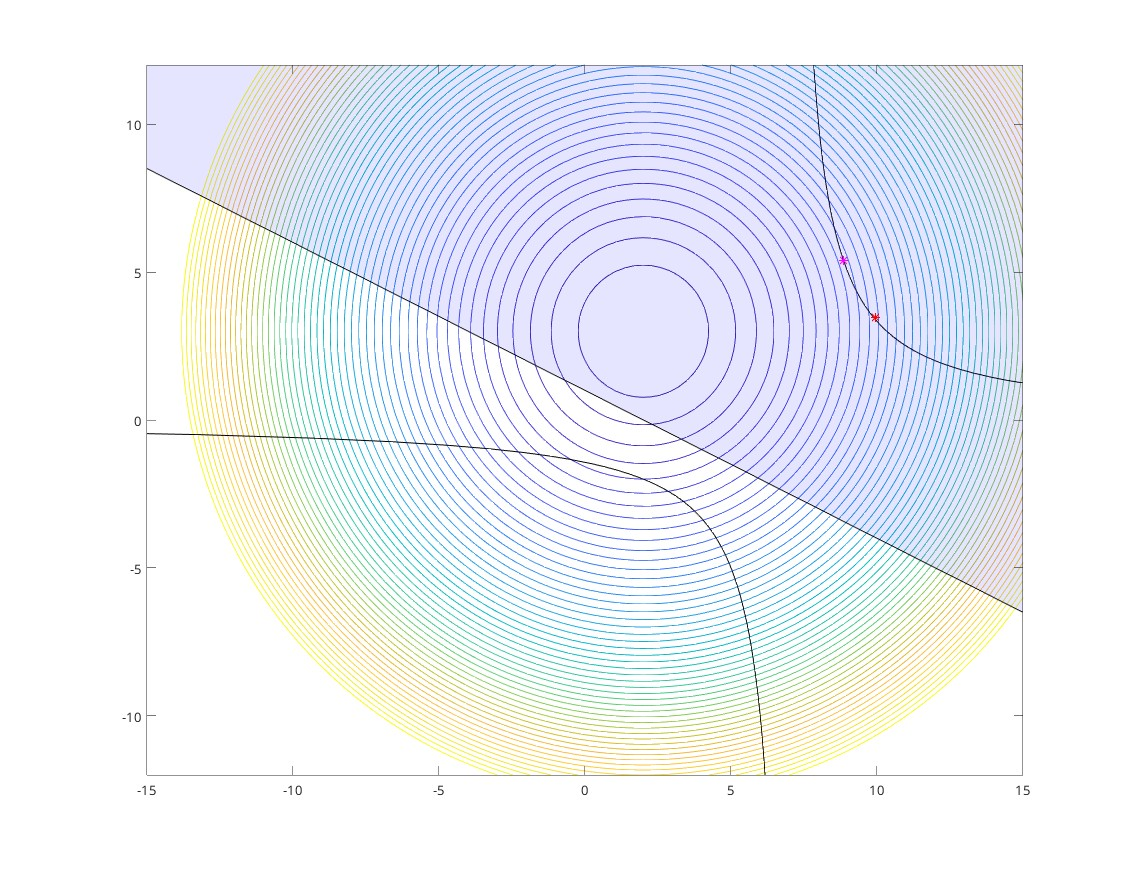
\includegraphics[width=0.75\textwidth]{images/relax3.jpg}
    \caption{The solution of the problem with relaxation order 3}
    \label{fig:constraints}
\end{figure}

\chapter{Laboratory 04: solution}
In this problem we assume that the plant to be identified is exactly described as a discrete-time
LTI models described by the following transfer function:
\[
G_p(q^{-1}) = \frac{N(q^{-1})}{D(q^{-1})} = \frac{\theta_3 + \theta_4 q^{-1} + \theta_5 q^{-2}}{1 + \theta_1 q^{-1} + \theta_2 q^{-2}} 
\]
\subsubsection{Data acquisition considerations:}
\begin{itemize}
    \item \textbf{Sampling rate: }As a rule of thumb, we should have at least 20 to 50 data from the transient of the system. Therefore, first, we apply a step to the system and we see the setteling time of the system, if this value is devided by 50 we obtain the period of the sampling. For this lab, setteling time is around 0.5, so the sampling rate should be at least 100. It was recommended to perform the lab with the sample rate around 250. \\
    It was also recommended to acquisit data with higher sampling rates such as 500 and 1000. It was suggested that we are going to face an issue regarding theoretical aspects of control thoery, yet to be explained. (I guess that maybe it makes the identification more dependent on the noise since we are introducing more noise to the data).
    \item \textbf{Bounds on the noise:} In order to have an idea about the bound of the noise, it was recommended to acquisit data with zero input, or at any rate without any input, and then, have an idea about the input and output noise bounds.
    \item \textbf{Input signal} It was recommended to use \textbf{uniformly distributed random signal}, but care should be taken regarding the amplitude of the noise. \begin{itemize}
                \item \textbf{too low amplitude} $\Rightarrow$ \textbf{bad SNR}, Signal to Noise Ratio.
                \item \textbf{too high amplitude} $\Rightarrow$ \textbf{Risk of saturation}, having non-linearity which is not assumed.\\
                \end{itemize}
                
                Considering the inputs with \textbf{DC gains}, so that you excite better the low-frequency range of frequency spectrum. Not too much! since a large DC and large amplitude may lead to saturation of the output. 
     
    \item In the lab assignment, it is required to stimulate the system with a square wave input, and acquire samples for identification purposes.
\end{itemize}


% ---------------------------------------------------------------------
% ---------------------------------------------------------------------
% ---------------------------------------------------------------------

% Declare appendix and set the equation counter format to (A.section.eqNumber)
\appendix
\renewcommand{\theequation}{\thesection.\arabic{equation}}
\input{chapters/Appendix}

\end{document}
